\ifnum\switch=1
% -----------------------------------------------------------------------------
% ------------------------------ Extended ToC ---------------------------------
% -----------------------------------------------------------------------------
\vspace{1.cm}
This chapter is based on the following references: \cite{BenFroNabSzy01, ChaMat94, DolJolNat15, EchLieSzyTic18, EchLieTic19, ElmSilWat14, FraLiuRooStyZho09, Gal13, Gan08, GolVan13, Gre97, GriDolSil15, Hac10, HorJoh12, KopOri10, LanRosSzy91, LieStr03, LieStr12, Lin10, MacOriShi00, MacOriShi02, MilOriShi96, Sch69, Saa03, Smi85, Sty05, TosWid05, Var09}.

\paragraph{Keywords:} Where do convection diffusion problems appear?, How are they discretized? What are the algebraic properties of their discretization?, What are the challenges for solving them?, How does the multiplicative Schwarz method work?, How does the (preconditioned) GMRES method work?


\section{Convection-Diffusion Problems}
\label{back:convdiff}

\noindent \textbf{Where do they appear?}
Modelling of transport phenomena.\\
\textbf{What are the challenges?}
Singularly perturbed problems. Boundary layers.\\
\textbf{How are conv-diff problems discretized?}
Shishkin meshes or adapted operators.\\

This section is based on the following references: \cite{EchLieSzyTic18, EchLieTic19, ElmSilWat14, GriDolSil15, Hac10, KopOri10, LanRosSzy91, LieStr03, Lin10, MilOriShi96, Saa03, Smi85, Sty05, Var09}.
\paragraph{Keywords:} Singularly perturbed problems, types of boundary layers, solution via adaptive meshes or adapted operators \cite{KopOri10, MilOriShi96}.


\subsection{Elliptic Operators}
\label{back:convdiff:elliptic}
This subsection is based on the following references: \cite{Hac10, KopOri10, LieStr03, MilOriShi96}.
\paragraph{Keywords:} classification of PDEs, general definition, boundary value problems, boundary conditions


\subsection{Finite Difference Methods}
This subsection is based on the following references: \cite{LanRosSzy91, Saa03, Smi85, Var09}.
\paragraph{Keywords:} Central differences, Upwind differences, five point stencil


\newpage
\subsection{Shishkin Mesh in 1D}
This subsection is based on the following references: \cite{FraLiuRooStyZho09, Lin10}.\\
\paragraph{Keywords:} Transition point, mesh generating function, Bakhvalov meshes


\subsection{Shishkin Mesh in 2D}
This subsection is based on the following references: \cite{FraLiuRooStyZho09, Lin10}.
\paragraph{Keywords:} Transition points in 2D


\subsection{Approximation of BVPs}
\label{back:convdiff:BVPapprox}
This subsection is based on the following references: \cite{GriDolSil15, Smi85}.
\paragraph{Keywords:} local truncation error, consistency, stability, convergence


\subsection{Properties of Discrete Convection-Diffusion Operators (\A)?}
\label{back:convdiff:A}
This subsection is based on the following references: \cite{EchLieSzyTic18, EchLieTic19}.
\paragraph{Keywords:} M-matrix, nonnormal, ill-conditioned, inverse monotonicity


\section{Iterative Solvers}
This section is based on the following references: \cite{BenFroNabSzy01, ChaMat94, DolJolNat15, Gan08, Gre97, LanRosSzy91, LieStr12, LieStr03, MacOriShi00, MacOriShi02, Sch69, Saa03, TosWid05, Var09}.
\paragraph{Keywords:} Iterative Vs Direct methods


\subsection{Classical Iterative Methods}
\label{back:itersolvers:class_sol}
This subsection is based on the following references: \cite{Saa03, Var09}.
\paragraph{Keywords:} Convergence factor, convergence radius, iteration matrix


\subsection{Krylov Subspace Methods}
\label{back:itersolvers:krylov}
This subsection is based on the following references: \cite{Gre97, LieStr12}.
\paragraph{Keywords:} Petrov-Galerkin framework, well defined method, GMRES, principles of convergence, mention stagnation of GMRES: \cite{LieStr03}, Eigenvalue analysis does not work


\subsubsection{Unpreconditioned GMRES Performance}
\label{back:itersolvers:krylov:unprec}

Eigenvalue analysis does not work.


\subsection{Domain Decomposition and Schwarz Methods}
\label{back:itersolvers:DDM}
This subsection is based on the following references: \cite{ChaMat94, DolJolNat15, Gan08, TosWid05}.
\paragraph{Keywords:} Basic ideas of domain decomposition


\subsubsection{The Continuous Case: Schwarz's Alternating Procedure}
\label{back:itersolvers:DDM:AltSchwarz}
This subsection is based on the following references: \cite{Gan08, MacOriShi00, MacOriShi02, Sch69}.
\paragraph{Keywords:} Procedure from Schwarz.


\subsubsection{The Discrete (Algebraic) Case: The Multiplicative Schwarz method}
\label{back:itersolvers:DDM:MultSchwarz}
This subsection is based on the following references: \cite{BenFroNabSzy01}.
\paragraph{Keywords:} Restriction operators, complementary projectors.


\section{Preliminaries of Linear Algebra}
This section is based on the following references: \cite{Gal13, GolVan13, HorJoh12, Saa03}.
\paragraph{Keywords:} Condition number, reorderings, M-matrices, projections, norms, permutations, preconditioning, (should this be the first section of this chapter?)

\else
% -----------------------------------------------------------------------------
% --------------------------- Content of Chapter ------------------------------
% -----------------------------------------------------------------------------

% The codes used in this thesis are the subject of Appendix~\ref{ch:matlab}

\section{Steady-State Convection-Diffusion Problems}
\label{back:convdiff}

Steady-state convection-diffusion problems arise in a wide range of
mathematical models which aim to describe a variety of phenomena appearing in
the natural world.
In the area of fluid flow, which is the most attributed area of science where
this equation plays an important role, they often appear in the linearization
of the Navier-Stokes equations as well as the Oseen equations \cite{BenOls06}
and they typically aim to describe the transport of a certain concentration
over a flow field. However, the range of application of these type of
problems includes many other models of physical phenomena, like it is the
case of the modeling of convective heat transport, the modeling of the
concentrations of chemicals in a chemical reactor \cite{GraKos74} as well as
modeling the oil extraction from underground reservoirs
\cite{ChaSunZheLu18}. Other physical phenomena, apparently unrelated to fluid
flow, such as the modeling of electronic transport in semiconductor materials
can also be described by such problems \cite{MarSzm89}.

In their most simple form, steady-state convection-diffusion problems are
described mathematically by the one-dimensional boundary value problem:
%
% \begin{equation}\label{eq:back:1Dbvp}
% -\epsilon  u''(x) + \omega u'(x)+\beta u(x) = f(x)\;  \text{ in }\; (0,1),\quad
% u(0)=g_0,\;\;u(1)=g_1,
% \end{equation}
\begin{equation}\label{eq:back:1Dbvp}
\begin{cases}
%-\epsilon  u''(x) + \omega u'(x)+\beta u(x) = f(x), & \text{in}\; (0,1)\\
-\epsilon\frac{\partial^2 u(x)}{\partial x^2}+\omega_x \frac{\partial u(x)}{\partial x} + \beta u(x)=f(x), & \text{in}\; (0,1)\\
\hspace{0.8cm} u(0)=g_0,\;\text{ and }\;u(1)=g_1, &
\end{cases}
\end{equation}
%
and more generally by its $n$-dimensional analogue:
%
% \begin{equation}\label{eq:back:nDbvp}
% -\epsilon \Delta u(\x) + \om \cdot \nabla u(\x)+\beta u(\x) = f(\x)\;
% % -\epsilon \Delta u + \om \cdot \nabla u +\beta u = f\;
% \text{ in }\; \Omega\in\Re^n,\quad
% u|_{\partial \Omega}=g.
% \end{equation}
\begin{equation}\label{eq:back:nDbvp}
\hspace*{2em}
\begin{cases}
-\epsilon \Delta u(\x) + \om \cdot \nabla u(\x)+\beta u(\x) = f(\x), &
\text{ in }\; \Omega\in\Re^n\\
%\;\;u|_{\partial \Omega}=g. &
\hspace{4.1cm} u(\x)=g(\x). & \text{ on }\; \partial \Omega.
\end{cases}
\end{equation}
%
% and its two-dimensional analogue:
% \begin{equation}\label{eq:back:2Dbvp}
% -\epsilon \Delta u(x,y) + \om \cdot \nabla u(x,y)+\beta u(x,y) = f(x,y)\;
% \text{ in }\; \Omega\in\mathbb{R}^2,\quad
% u|_{\partial \Omega}=g,
% \end{equation}
The partial differential equation (PDE) in \eqref{eq:back:1Dbvp} or
\eqref{eq:back:nDbvp} is classified as a linear second-order elliptic PDE
(see Section~\ref{back:convdiff:elliptic}) where
the term $\om\cdot\nabla u(\x)$ in \eqref{eq:back:nDbvp} models convection and
the term $-\epsilon\Delta u(\x)$ models diffusion. In most applications the
parameter $\epsilon>0$ is small, typically in the range $\mathscr{O}(10^{-2})$ to $\mathscr{O}(10^{-8})$
while the magnitude of the flow field $\|\om\|$ is typically of
$\mathscr{O}(1)$, so that very often \emph{convection dominates diffusion}.
More specifically, in order to have a relative measure of which term is more
dominant than the other it is common to introduce the \emph{Peclet number},
$\text{Pe}$. If $L$ is a length associated with the domain $\Omega$ (length of
the interval in 1D, longest length inside the domain for 2D, etc.), then
%
\begin{equation}\label{eq:back:Peclet}
\text{Pe}=
\frac{L}{\epsilon}\max\left\{|\omega_x|,|\omega_y|,\ldots,|\omega_d|\right\},
\end{equation}
%
where $\omega_x,\omega_y,\ldots\omega_d$ are the components of $\om$ and thus
for most practical cases $\text{Pe}\gg1$, constituting what is known as a
singularly perturbed PDE.
%
% It is widely accepted that the numerical modeling of convection dominated problems is quite challenging in contrast to diffusion dominated problems, but challenges appear in both types of regimes. We can understand these challenges by examining the terms of the convection diffusion operator in \eqref{back:eq:back:1Dbvp} or \eqref{eq:back:nDbvp}. If we neglect the first order temrms in the operator, we obtain what is known as \emph{Poisson problems}, and we can compare the difference of both types of problmes:
%
% % I'll start with some favorable qualities of diffusion problems, and then mention why they are not present for advection problems:
% \begin{enumerate}
%   \item Discretizations are often symmetric and definite. If they aren't symmetric then they still are usually definite. - this enables use of better linear solvers in some cases.
%
%   \item Smoothness of solutions is often guaranteed under very relaxed assumptions on input data (source term, boundary conditions). This isn't always true, but it often is.
%
%   \item Scale separation: it's often possible to separate small-scale behavior from large-scale behavior. This allows preconditioners/solvers like multigrid where different scales of physics are targeted by different levels of the preconditioner.
% \end{ennumerate}
%
% On the other hand, if we neglect the second oreder terms in \eqref{back:eq:back:1Dbvp} or \eqref{eq:back:nDbvp} we obtain a purely convective problem, whith some properties:
% \begin{enumerate}
%   \item Discretizations rarely result in symmetric and definite matrix. Can potentially be indefinite.
%
%   \item   Much fewer smoothness guarantees. This is problem dependent.
%
%   \item  (almost) impossible to numerically separate scales. Stability requires you always resolve the smallest scale, which is often expressed as a relationship between grid spacing and advection speed. This means classic multigrid strategies won't work because the coarse grid will be aliased. In some cases this isn't strictly true because the "fine grid" may be very over-resolved compared to advection speed because of things like discontinuous coefficients, and in those cases multigrid may work, but only if the coarse grid respects the stability conditions.
% \end{ennumerate}
% But in other respects, advection problems can actually be easier than diffusion problems. It really depends on what you want.
%
% time-dependent Advection problems are usually easier to get time-accurate solutions for than diffusion problems, because they often only involve first derivatives and this results in favorable CFL condition (again, depending only on advection speed). You start to lose this advantage when your discretization has variable order of accuracy, though.
%
% If you use implicit time-stepping then the matrix conditioning is often better than a similarly discretized diffusion problem.

The region $\Omega$ can be any reasonable domain in $n$-dimensions and the velocity field $\om$, which throughout this work will be considered as incompressible (i.e., we assume that $\nabla \cdot \om = 0$), is used as reference to partition the boundary of the domain, $\partial \Omega$, as follows:
%
\begin{equation}\label{eq:back:bc}
\begin{array}{rl}
\partial\Omega_{+} = \{\x\text{ on }\partial\Omega \;|\;
\om(\x)\cdot\n(\x)>0\},
& \text{the \emph{outflow boundary,}}\\
\partial\Omega_{0} = \{\x\text{ on }\partial\Omega \;|\;
\om(\x)\cdot\n(\x)=0\},
& \text{the \emph{characteristic boundary,}}\\
\partial\Omega_{-} = \{\x\text{ on }\partial\Omega \;|\;
\om(\x)\cdot\n(\x)<0\},
& \text{the \emph{inflow boundary,}}\\
\end{array}
\end{equation}
where $\n(\x)$ denotes the unit outward pointing normal vector to the boundary
at the point $\x$.

Since a typical value of $\epsilon$ in a convection dominated problem is
of~$\mathscr{O}(10^{-6})$, the influence of the diffusion term is very small and the solution $u$ to \eqref{eq:back:nDbvp} is usually very close to the solution $\hat{u}$ of the equation:
%
\begin{equation}\label{eq:back:reducedprob}
\om \cdot \nabla \hat{u}(\x)+\beta \hat{u}(\x) = f(\x),
\end{equation}
%
commonly known as the \emph{reduced problem}. It is important to note that the highest order derivative in equation \eqref{eq:back:reducedprob} is of lower order than that of \eqref{eq:back:nDbvp}, and its solution $\hat{u}$ will most likely not be able to satisfy all the boundary conditions imposed on the original problem. In order to do so, the solution $u$ to the convection-diffusion BVP usually presents sharp gradients close to the outflow boundary of the domain and $u$ is said to have have an \emph{exponential boundary layer} along the outflow boundary $\partial\Omega_{+}$. Sharp gradients of the solution may also appear in the interior portion of $\Omega$ if any number of
discontinuities are present in the boundary conditions set on $\partial\Omega_{-}$. The diffusion term takes care of smoothing such discontinuities into a
continuos but steep \emph{characteristic/internal boundary layer}. The appearance of both types of boundary layers represent the main challenge when constructing numerical approximations to the solutions of \eqref{eq:back:1Dbvp} and \eqref{eq:back:nDbvp} and constitutes the main reason why
most numerical methods will not work satisfactorily when solving these type of
problems; see~\cite{Mor96}. Thus, the accurate solution of such problems requires the use of
special discretization techniques and/or the use of specially
\emph{fitted methods} which modify the linear operator in
\eqref{eq:back:nDbvp} in order to guarantee the stability of a numerical
method~\cite{Sty13}. A general overview of accurate solution techniques can be found, e.g.,
in the survey article~\cite{Sty05} or in the
monographs~\cite{Lin10, RooStyTob08}. One widely accepted discretization
technique in this context, and which represents the main focus of this work, is
given by using upwind or central finite difference schemes posed on a Shishkin
mesh as described, e.g., in~\cite[\S~5]{Sty05}
or~\cite{FarHegMilOriShi00,KopOri10,LinSty01,MilOriShi96}.

\subsection{Elliptic Operators}
\label{back:convdiff:elliptic}

In its most general form, a linear second-order partial differential equation
can be written as
%
\begin{equation}\label{eq:back:cont_linsys}
\hat{\mathscr{A}}\hat{u}=\hat{f}.
\end{equation}
%
Usually the PDE holds on a domain $\Omega\in\mathbb{R}^2$ where the operator  $\hat{\mathscr{A}}$ can be written as
%
\begin{equation}\label{eq:back:cont_oper}
\hat{\mathscr{A}}\equiv a \frac{\partial^2 }{\partial x^2} + 2b \frac{\partial^2 }{\partial x\partial y} + c \frac{\partial^2 }{\partial y^2} + p\frac{\partial }{\partial x} + q \frac{\partial }{\partial y} + r,
\end{equation}
%
where the coefficients $a,b,c,p,q,r$ usually depend on both space variables $x$ and $y$. The behavior of the solutions to \eqref{eq:back:cont_linsys}
is usually determined by the highest order derivatives in the operator $\hat{\mathscr{A}}$ so for the sake of discussion and without loss
of generality we will consider $p=q=r=0$  and $a\geq0$. There are three
alternatives for classifying such operators (see \cite{ElmSilWat14, Eva10} for a detailed description of the classification of PDEs), which are
%
\begin{equation}\label{eq:back:PDEclass}
\begin{array}{ll}
b^2-4ac>0, & \text{\emph{Hyperbolic-type,}}\\
b^2-4ac=0,\,a>0, & \text{\emph{Parabolic-type,}}\\
b^2-4ac<0, & \text{\emph{Elliptic-type.}}\\
\end{array}
\end{equation}

The convection-diffusion equation in \eqref{eq:back:nDbvp} defines a linear
second order differential operator of elliptic-type, given by:
%
\begin{equation}\label{eq:back:ellipticPDE}
%\mathscr{A}u\equiv-(au_{xx}+2bu_{xy}+cu_{yy})+pu_x+qu_y+ru,
\mathscr{A}u\equiv
%-\epsilon(u_{xx}+u_{yy})+\omega_xu_x+\omega_yu_y+\beta u,
-\epsilon\left( \frac{\partial^2 u}{\partial x^2} + \frac{\partial^2 u}{\partial y^2}\right) + \omega_x\frac{\partial u}{\partial x} + \omega_y \frac{\partial u}{\partial y} + \beta u
\end{equation}
where, in general, the coefficients $\epsilon,\omega_x,\omega_y$ and $\beta$
represent functions of the space variables $x$ and $y$. Very often in practice,
and throughout this work, they will be considered constant unless otherwise
specified. In order to have a uniquely defined solution an appropriate condition must be specified at each point of the boundary $\partial\Omega$. By partitioning the boundary into three disjoint sets $\Gamma_i$, $i=1,2,3$ with
$\partial \Omega=\Gamma_1\cup\Gamma_2\cup\Gamma_3$, and $\n(\x)$
denotes the unit outward normal vector to $\partial\Omega$ at the point
$\x=(x,y)$ then the boundary conditions are given by
\begin{equation}
\begin{array}{rrl}
u(\x) = g(\x), & \x\in\Gamma_1, & \text{\emph{Dirichlet,}}\\
\n(\x)\cdot \nabla u(\x) = g(\x),& \x\in\Gamma_2, & \text{\emph{Neumann,}}  \\
\gamma(\x)u(\x) + \delta(\x)\n(\x)\cdot\nabla u(\x) = g(\x), & \x\in\Gamma_3, & \text{\emph{Robin,}}
\end{array}
\end{equation}
where $\gamma, \delta$, and  $g$ are known functions. More generally, the
boundary conditions can be written in compact form as $\mathscr{B}u=g$ so that the boundary value problem can be written as $\mathcal{A}u=\mathcal{F}$, where
%
\begin{equation}\label{eq:back:ellipticBVP}
\mathcal{A}u=\begin{cases}
\mathscr{A}u &\text{in}\quad \Omega,\\
\mathscr{B}u &\text{on}\quad \partial\Omega,
\end{cases},
\quad\text{and}\quad
\mathcal{F}=\begin{cases}
f &\text{in}\quad \Omega,\\
g &\text{on}\quad \partial\Omega.
\end{cases}
\end{equation}
In further sections of this work we will only treat problems with Dirichlet
boundary conditions.

\subsection{Finite Difference Methods}
\label{back:convdiff:findiff}

The aim of numerical approximation methods for solving PDEs is to construct
accurate numerical solutions to BVPs of the form \eqref{eq:back:ellipticBVP} that may or may not have analytical
solutions. Of the available methods, those employing finite differences or
finite elements are more frequently used and more universally applicable than
any other, although finite elements are not considered in this work. For an
excellent treatment of solving BVPs with finite elements please refer to the
monograph \cite{ElmSilWat14}, for a comprehensive survey on the theory of
finite elements see \cite{Bra07}.

In short, in a finite  difference method a set of mesh of points is introduced
within the domain of definition of the BVP and then any derivatives appearing
in the PDE or boundary conditions are replaced by finite difference
approximations at the mesh points. Thus, finite difference methods are
approximate in the sense that derivatives \emph{at a point} are approximated
by difference quotients \emph{over a small interval}, i.e., $u_x =\partial u/
\partial x$ is replaced by $\Delta u/\Delta x$ where $\Delta x$ is small and
$y$ is constant, but they are \emph{not} approximate in the sense of being
crude estimates. In the following we will  describe the method for a
two-dimensional model problem.

As much as the analytic solution of the BVP is a function $u$ defined on
a domain $\Omega$, say $[0,1]\times[0,1]$, finite difference methods seek a
numerical solution only at a finite number of grid points:
\[
\Omega_D = \{(x_i,y_j):i=0,\ldots,N;j=0,\ldots, M\}.
\]
The grid points on the boundary are denoted by $\partial\Omega_D$, and the
entire grid by $\overline{\Omega}_D=\Omega_D\cup\partial \Omega_D$. We can evaluate the exact solution of the BVP on the introduced points to obtain the values
\begin{align*}
\begin{array}{cccc}
u(x_0,y_M) & u(x_1,y_M) & \ldots & u(x_N,y_M)\\
  \vdots   &   \vdots   &        &   \vdots  \\
u(x_0,y_1) & u(x_1,y_1) & \ldots & u(x_N,y_1)\\
u(x_0,y_0) & u(x_1,y_0) & \ldots & u(x_N,y_0).\\
\end{array}
\end{align*}
The finite difference approximation scheme replaces the given BVP with a set
of $(N+1)~\times~(M+1)$ finite difference equations in $(N+1)~\times~(M+1)$
unknowns. The function $u^D$, commonly referred to as  a \emph{grid function}
is only defined on the set of grid points $\overline{\Omega}_D$ and its value
at the grid point $\x_{i,j}=(x_i,y_j)$ is denoted by $u^D_{i,j}$.
\begin{align*}
\begin{array}{cccc}
u^D_{0,M} & u^D_{1,M} & \ldots & u^D_{N,M}\\
\vdots  & \vdots  &        & \vdots \\
u^D_{0,1} & u^D_{1,1} & \ldots & u^D_{N,1}\\
u^D_{0,0} & u^D_{1,0} & \ldots & u^D_{N,0}
\end{array}
\end{align*}
The solution to the finite difference equations can then be identified with the
grid function $u^D$, whose value $u^D_{i,j}$ at a typical point $\x_{i,j}=(x_i,y_j)\in\Omega_D$ approximates the exact solution $u_{i,j} \equiv u(x_i,y_j)$ at that point. The values of $u^D$ at the internal grid points are found by solving the system of finite difference equations while the values of $u^D$ at the boundary nodes are known from the Dirichlet conditions. The premise of the method being that each element from the set $u^D_{0,0},\ldots, u^D_{N,M}$ should converge to its corresponding element in $u(x_0,y_0),\ldots, u(x_N,y_M)$ as $N,M\rightarrow\infty$.
%
\begin{figure}[h!]
\centering
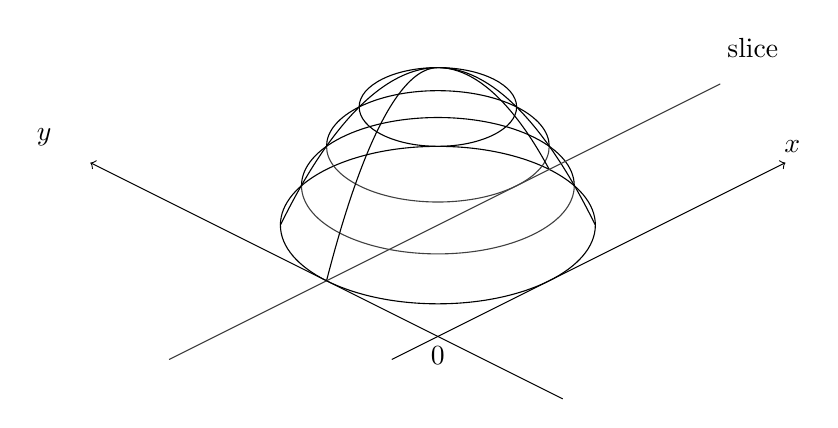
\begin{tikzpicture}[scale=1,yscale=.5]

\draw (0,0) arc (180:0:2);
\draw ({2-sqrt(3)},1) arc (180:0:{sqrt(3)});
\draw ({2-sqrt(2)},2) arc (180:0:{sqrt(2)});
\draw (1,3) arc (180:0:1);

\draw (0,0) arc (-180:0:2);
\draw[darkgray] ({2-sqrt(3)},1) arc (-180:0:{sqrt(3)});
\draw[darkgray] ({2-sqrt(2)},2) arc (-180:0:{sqrt(2)});
\draw (1,3) arc (-180:0:1);

\draw (0,0) parabola bend (2,4) (4,0);
\draw ({2-sqrt(2)},{-sqrt(2)}) parabola bend (2,4) ({2+sqrt(2)},{sqrt(2)});

\draw ({2},{-2*sqrt(2)}) node [below] {0};
\draw[darkgray] ({2-sqrt(2)},{-sqrt(2)}) --++ (5,5);
\draw[darkgray] ({2-sqrt(2)},{-sqrt(2)}) --++ (-2,-2);
\draw (6,5) node [below] {slice};
\draw [->]({2+sqrt(2)},{-sqrt(2)}) --++ (3,3);
\draw ({6.5},{2}) node {$x$};
\draw ({2+sqrt(2)},{-sqrt(2)}) --++ (-2,-2);
\draw [->]({2-sqrt(2)},{-sqrt(2)}) --++ (-3,3);
\draw ({2-sqrt(2)},{-sqrt(2)}) --++ (3,-3);
\draw ({-3},{2.7}) node [below] {$y$};
\end{tikzpicture}
\caption{Generic function of two variables with sufficiently many derivatives.}
\label{fig:back:generic_f}
\end{figure}
%
% \begin{tikzpicture}[scale = 0.3]
%   \begin{axis}[view={-20}{20}, grid=both]
%     \addplot3[surf,opacity=0.8,samples=50, samples y=30,domain=-3.5:3.5,domain y=-1:1] % z buffer=sort, colormap/whitered,
% {(x-0)^2-(y-0)^2};
% %{((x+sin(deg(x)))^2};
%     %] file {filename.txt};
%     %\addplot3[surf, point meta=explicit] table [z expr=0.5, meta index=2] {filename.txt};
%   \end{axis}
% \end{tikzpicture}

The interchange of differential equations and their boundary conditions by
algebraic equations in the finite difference method is accomplished by analyzing the Taylor series expansions at each point.
To exemplify this process we will assume that the function $v(\x)=v(x,y)$ possesses enough continuous derivatives for the Taylor series expansions to be well defined. An example of such a function is given in Figure~\ref{fig:back:generic_f}
%\td{need to figure out a way to make a nice 3D plot of an $f$ with many derivatives}.
%
\begin{figure}[h!]
\centering
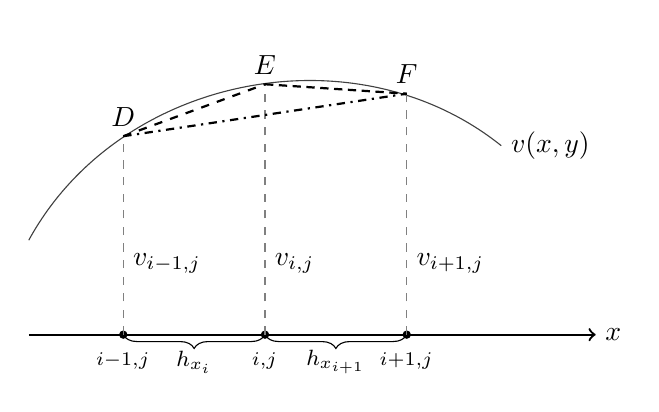
\begin{tikzpicture}[scale = 0.6]
%%%%% x-axis:
\draw[thick,->] (0,1) -- (12, 1);
\node[right] at (12,1) {$x$};
%%%%% function
\draw[darkgray] (0,3) to [bend left=50] (10,5);
%\draw (0,3) .. controls (0,4) and (0,8) .. (10,5);
\node[right] at (10,5) {$v(x,y)$};
%%%%% Black nodes and dots on x-axis:
\draw[black,fill=black] (2,1) circle (0.5ex);
\node[below,yshift=-3pt] at (2,1) {$\x_{i-1,j}$};
\draw[black,fill=black] (5,1) circle (0.5ex);
\node[below,yshift=-3pt] at (5,1) {$\x_{i,j}$};
\draw[black,fill=black] (8,1) circle (0.5ex);
\node[below,yshift=-3pt] at (8,1) {$\x_{i+1,j}$};
%%%%% h's:
% \node[below] at (3.5,1) {$h_{x}_{i}$};
% \node[below] at (6.5,1) {$h_{i+1}$};
%%%%%% braces:
\draw [decorate,decoration={brace,amplitude=5pt},xshift=0pt,yshift=0pt] (5,1) -- (2,1) node [black,midway,yshift=-10pt] {\footnotesize $h_{x_i}$};
\draw [decorate,decoration={brace,amplitude=5pt},xshift=0pt,yshift=0pt] (8,1) -- (5,1) node [black,midway,yshift=-10pt] {\footnotesize $h_{x_{i+1}}$};
%%%%% Vertical dashed lines, with labels and crosses
\draw[gray, dashed] (2, 1) -- (2, 5.2);
\node[right] at (2, 2.5) {$v_{i-1,j}$};
\node at (2, 5.2) {\cross};
\node[above] at (2, 5.2) {$D$};
\draw[gray, dashed] (5,1) -- (5, 6.3);
\node[right] at (5, 2.5) {$v_{i,j}$};
\node at (5, 6.3) {\cross};
\node[above] at (5, 6.3) {$E$};
\draw[gray, dashed] (8,1) -- (8, 6.1);
\node[right] at (8, 2.5) {$v_{i+1,j}$};
\node at (8, 6.1) {\cross};
\node[above] at (8, 6.1) {$F$};
%%%%% Chords:
\draw[thick,dashed] (2, 5.2) -- (5, 6.3);
\draw[thick,densely dashed] (5, 6.3) -- (8, 6.1);
\draw[thick,dash dot] (2, 5.2) -- (8, 6.1);
\end{tikzpicture}
\caption{One-dimensional slice of the function depicted in Figure~\ref{fig:back:generic_f}. The chords $DE$, $EF$ and $DF$ are different possibilities of approximating the slope of the tangent at the point $E$.}
\label{fig:back:derivatives_f}
\end{figure}
%
% \begin{figure}[h!]
% \centering
% 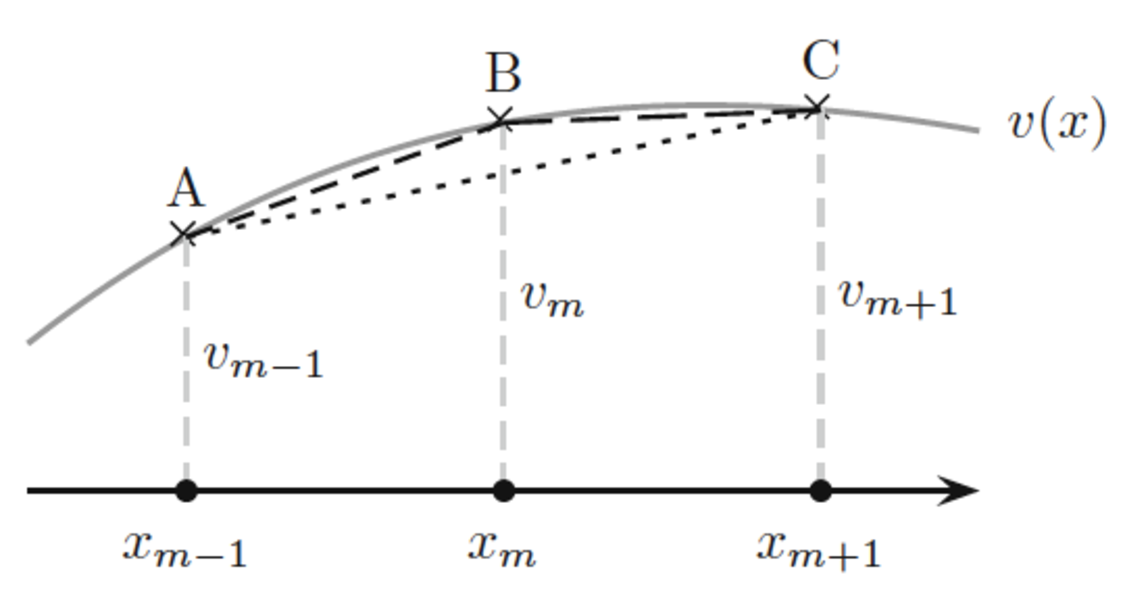
\includegraphics[width=0.5\linewidth]{figures/derivatives.pdf}
% \caption{The gradients of the chords $AB$ (backward), $BC$ (forward) and $AC$
% (central) are three possibilities of approximating the gradient of the tangent
% to the function $v(x)$(solid curve) at $B$.}\label{fig:back:derivatives_f}
% \end{figure}
%

Figure~\ref{fig:back:derivatives_f} represents a slice
of the function pictured in Figure~\ref{fig:back:generic_f} for a constant
value of $y$, the gradient of the function $v(\x)=v(x,y)$ at point $E$
($\x_{i,j}=(x_i,y_j)$) in the $x$-direction may be  approximated by the
gradients of any of the three chords $DE$, $EF$, or $DF$, each  case with its own degree of approximation. The slope of the backward chord at the point $E$
($\x_{i,j}=(x_i,y_j)$) can be associated to the the following one-directional
Taylor expansion in two-dimensions:
%
\begin{equation}\label{eq:back:1Dtaylor}
v(x-\Delta x,y)=v(x,y)-\frac{\partial v(x,y)}{\partial x}\Delta x + \frac{\partial^2 v(\xi,y)}{\partial x^2}\frac{\Delta x^2}{2},
\end{equation}
%
for some number $\xi\in\left((x,y),(x+\Delta x,y)\right)$, we choose the point
$\x_{i,j}=(x_i,y_j)$ and
%, adopting a notation \td{there is conflict with notation of partial derivatives and subindices}
%where $v_{i,j}$, $v_{x}(x_i,y_j)$ and $v_{xx}(x_i,y_j)$ are used to denote
%$v(x_i,y_j)$, $\frac{\partial v(x_i,y_j)}{\partial x}$, and
%$\frac{\partial^2 v(x_i,y_j)}{\partial x^2}$ respectively, we can
rearrange the previous expression to give:
$$
%v_{x}(x_i,y_j) =
\frac{\partial v(x_i,y_j)}{\partial x} = h_{x_i}^{-1}(v_{i,j}-v_{i-1,j}) + \frac{h_{x_i}}{2}\frac{\partial^2 v(\xi_i,y_j)}{\partial x^2}, \quad \xi_i\in(x_{i-1},x_{i}),
$$
where the subscript $i$ in $\xi_i$ reflects its dependence on $(x_i,y_j)$.
We have
$$
%v_x(x_i,y_j) =
\frac{\partial v(x_i,y_j)}{\partial x} = h_{x_i}^{-1}(v_{i,j}-v_{i-1,j})+R_{i,j} = h_{x_i}^{-1}(v_{i,j}-v_{i-1,j}) + \mathscr{O}(h_{x_i}).
$$

The remainder term, commonly referred to as the \emph{local truncation error}
$R_{i,j}$ (see~\cite{PapLieStr14} for a good discussion of error
distributions), corresponds to truncating the Taylor series
\eqref{eq:back:1Dtaylor}. When the local truncation error is neglected, we obtain the \emph{backward difference approxiamtion} of
$\frac{\partial v(x_i,y_j)}{\partial x}$ at the point $\x_{i,j}=(x_i,y_j)$.
The backward difference operator or \emph{upwind finite difference operator}
in the $x$-direction, $\Delta^{-}_{x}$, is defined by
%
\begin{equation}\label{eq:back:1DupwindOp}
\Delta^{-}_{x}v_{i,j}\equiv v_{i,j}-v_{i-1,j},
\end{equation}
%
and so $\frac{\partial v(x_i,y_j)}{\partial x} \approx h_{x_i}^{-1}
\Delta^{-}_{x}v_{i,j}$ with an error $\mathscr{O}(h_{x_i})$.

We chose the expansion \eqref{eq:back:1Dtaylor}, however we can proceed in a
similar fashion using the forward version of the Taylor series instead:
\begin{equation}\label{eq:back:1Dtaylor_b}
v(x+\Delta x,y)=
%v(x,y)+v_{x}(x,y)\Delta x + v_{xx}(\xi,y)\frac{\Delta x^2}{2},
v(x,y)+\frac{\partial v(x,y)}{\partial x}\Delta x + \frac{\partial^2 v(\xi,y)}{\partial x^2}\frac{\Delta x^2}{2}
\end{equation}
and by defining the \emph{forward finite difference operator} in the
$x$-direction, $\Delta^{+}_{x}$,
\begin{equation}\label{eq:back:1DforwardOp}
\Delta^{+}_{x}v_{i,j}\equiv v_{i+1,j}-v_{i,j},
\end{equation}
%
we obtain another approximation to the derivative of $v$ at the point
$\x_{ij}$,\linebreak $\frac{\partial v(x_i,y_j)}{\partial x} \approx h_{x_{i+1}}^{-1}
\Delta^{+}_{x}v_{i,j}$ now with an error of $\mathscr{O}(h_{x_{i+1}})$.

Finally, by defining the \emph{central finite difference operator} in the
$x$-direction, $\Delta^{0}_{x}$,
\begin{equation}\label{eq:back:1DcentralOp}
\Delta^{0}_{x}v_{i,j}\equiv v_{i+1,j}-v_{i-1,j},
\end{equation}
%
we find that $\frac{\partial v(x_i,y_j)}{\partial x}
\approx (h_{x_{i}} + h_{x_{i+1}})^{-1} \Delta^{0}_{x}v_{i,j}$
now with an error $\mathscr{O}\left((h_{x_{i}} + h_{x_{i+1}})^2\right)$. It is
possible to obtain more accurate approximations by including more terms
in the Taylor series \eqref{eq:back:1Dtaylor} and \eqref{eq:back:1Dtaylor_b}
before truncating it, obtaining higher order methods (see \cite{Dem97} for a
discussion in this direction).
% \td{\textbf{write}: still need to add derivation of the formulas for second derivatives}

In order to approximate second order derivatives (and most even-order derivatives), it is common to introduce another ``artificial" central approximation
\begin{equation}\label{eq:back:1DcentralOp}
\delta_{x}v_{i,j}\equiv v_{i+\frac12,j}-v_{i-\frac12,j},
\end{equation}
which makes use of intermediate points which are not on the grid. This approximation corresponds to the $\Delta$ approximation with a half-step $h_{x_i}/2$.
 Nevertheless, by computing $\delta_x(\delta_x)v_{i,j}$ we obtain
\begin{equation}\label{eq:back:1DcentralOp}
\delta_{x}(\delta_x v_{i,j})= v_{i+1,j}-2v_{i,j}+v_{i-1,j}.
\end{equation}
In the exact fashion as above, by considering both Taylor approximations \eqref{eq:back:1Dtaylor} and \eqref{eq:back:1Dtaylor_b}, adding them together adn evaluatng at the point $\x_{i,j}$ we obtain a centered finite difference approximation to the second derivative,
\begin{equation*}
\frac{\partial^2 v(x_i,y_j)}{\partial x^2} = h_{x_i}^{-2}(v_{i+1,j}-2v_{i,j}+v_{i-1,j})- \mathscr{O}(h_{x_i}^2)\approx h_{x_i}^{-2}\delta^2v_{i,j},
\end{equation*}
with a remainder term proportional to $h_{x_i}^2$.

This analysis can be repeated for approximating the partial derivative of the
function $v$ in the $y$-direction to obtain analogous results. Using the notation $v_{x}=\frac{\partial v}{\partial x}$, $v_{xx}=\frac{\partial^2 v}{\partial x^2}$, and where $h_{x_{\text{eff}}}=h_{x_i}+h_{x_{i+1}}$ we
summarize the results in Table~\ref{tab:back:findiff}

%\begin{table}[h!]\centering
\begin{equation}\label{tab:back:findiff}
\begin{array}{ll}
%\hline
%$1^{\text{st}}$ Order Forward operator in $x$-dir &
\Delta^{+}_{x} v_{i,j} = v_{i+1,j} - v_{i,j} = h_{x_{i+1}} v_{x} + \frac{1}{2}h_{x_{i}}^2 v_{xx} + \mathscr{O}(h_{x_{i+1}}^3) &
\text{\emph{Forward differences}} \\
% %\hline
% $1^{\text{st}}$ Order Forward operator in $y$-dir & $
\Delta^{+}_{y} v_{i,j} = v_{i,j+1} - v_{i,j} = h_{y_{i+1}} v_{y} + \frac{1}{2}h_{y_{i}}^2 v_{yy} + \mathscr{O}(h_{y_{i+1}}^3) &
\text{\emph{Forward differences}}\\
%\hline
%$1^{\text{st}}$ Order Upwind operator in $x$-dir &
\Delta^{-}_{x} v_{i,j} = v_{i,j} - v_{i-1,j} = h_{x_{i}} v_{x} - \frac{1}{2}h_{x_{i}}^2 v_{xx} + \mathscr{O}(h_{x_{i}}^3) &
\text{\emph{Upwind differences}} \\
% %\hline
% $1^{\text{st}}$ Order Upwind operator in $y$-dir & $
\Delta^{-}_{y} v_{i,j} = v_{i,j} - v_{i,j-1} = h_{y_{i}} v_{y} - \frac{1}{2}h_{y_{i}}^2 v_{yy} + \mathscr{O}(h_{y_{i}}^3) &
\text{\emph{Upwind differences}}\\
% %\hline
% %$1^{\text{st}}$ Order Central operator in $x$-dir &
\Delta^{0}_{x} v_{i,j} = v_{i+1,j} - v_{i-1,j} = h_{x_{\text{eff}}} v_{x} +
\frac{1}{6}h_{x_{\text{eff}}}^3 v_{xxx} + \mathscr{O}(h_{x_{\text{eff}}}^5) &
\text{\emph{Central differences}} \\
% %\hline
% $1^{\text{st}}$ Order Central operator in $y$-dir  & $
\Delta^{0}_{y} v_{i,j} = v_{i,j+1} - v_{i,j-1} = h_{y_{\text{eff}}} v_{y} + \frac{1}{6}h_{y_{\text{eff}}}^3 v_{yyy} + \mathscr{O}(h_{y_{\text{eff}}}^5) &
\text{\emph{Central differences}} \\
% %\hline
% %$2^{\text{nd}}$ Order Central operator in $x$-dir &
\delta^{2}_{x} v_{i,j} = v_{i+1,j} - 2v_{i,j}+v_{i-1,j} = h_{x_{\text{eff}}}^2 v_{xx} + \frac{1}{12}h_{x_{\text{eff}}}^4 v_{xxxx} + \mathscr{O}(h_{x_{\text{eff}}}^6) &
\text{\emph{Central differences}} \\
% %\hline
% $2^{\text{nd}}$ Order Central operator in $y$-dir & $
\delta^{2}_{y} v_{i,j} = v_{i,j+1} - 2v_{i,j} + v_{i,j-1} = h_{y_{\text{eff}}}^2 v_{yy} + \frac{1}{12}h_{x_{\text{eff}}}^4 v_{yyyy} + \mathscr{O}(h_{y_{\text{eff}}}^6) &
\text{\emph{Central differences}}
% %\hline
\end{array}
\end{equation}
%\caption{Finite difference operators and Taylor Expansions $(h_{y_{\text{eff}}}=h_{y_{i}}+h_{y_{i+1}})$.}
%\end{table}

\subsection{Shishkin Mesh in 1D}
\label{back:convdiff:shihs1D}

In order to obtain an accurate numerical solution of BVPs with singularly
perturbed convection-diffusion problems described by equation
\eqref{eq:back:1Dbvp}, we require special discretization techniques.
As mentioned in Section~\ref{back:convdiff}, we focus on the approach of
using upwind or central finite difference schemes posed on a Shishkin mesh, an
approach described described, e.g., in~\cite[\S~5]{Sty05}
or~\cite{FarHegMilOriShi00,KopOri10,LinSty01,MilOriShi96}. In this subsection
we introduce the one-dimensional Shishkin mesh and describe its construction.
For a comprehensive treatment of layer-adapted meshes for convection-diffusion
problems see the monograph \cite{Lin10}. Without loss of generality, we assume
that $\omega_x\gg \epsilon >0$ and $\beta\geq 0$ and that the parameters of
the problem \eqref{eq:back:1Dbvp}, i.e., $\epsilon,\omega_x,\beta,f,g_0,$ and
$g_1$, are chosen so that the solution $u(x)$ has one boundary layer close to
the point $x=1$.
% \td{\textbf{fix}: the underbrace for $h_{x}$ in the Figure~\ref{fig:back:shmesh1D} looks weird.}
%
\begin{figure}[h!]
\centering
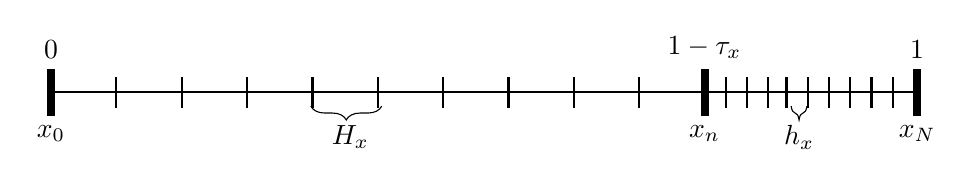
\begin{tikzpicture}
%%%%% x-axis:
\draw[thick,-] (0,1) -- (11, 1);
\draw[thick,line width=1mm] (0,0.7)   -- (0, 1.3);
\draw[thick,line width=1mm] (11,0.7)  -- (11, 1.3);
\draw[thick,line width=1mm] (8.3,0.7) -- (8.3, 1.3);
\foreach \i in {.83,1.66,2.49,3.32,4.15,4.98,5.81,6.64,7.47}{
  \draw[thick,-] (\i,0.8) -- (\i, 1.2);
}
\foreach \ii in {8.57,8.84,9.11,9.34,9.61,9.88,10.15,10.42,10.69}{
  \draw[thick,-] (\ii,0.8) -- (\ii, 1.2);
}
\node[below] at (0,0.7)  {$x_{0}$};
\node[above] at (0,1.3)  {$0$};
\node[below] at (11,0.7) {$x_{N}$};
\node[above] at (11,1.3) {$1$};
\node[below] at (8.3,0.7) {$x_{n}$};
\node[above] at (8.3,1.3) {$1-\tau_x$};
\draw [decorate,decoration={brace,amplitude=5pt},xshift=0pt,yshift=-5pt] (4.2,1) -- (3.3,1) node [black,midway,yshift=0pt] {};
\node[below] at (3.8,0.7) {$H_{x}$};
\draw [decorate,decoration={brace,amplitude=5pt},xshift=0pt,yshift=-5pt] (9.6,1) -- (9.4,1) node [black,midway,yshift=0pt] {};
\node[below] at (9.5,0.7) {$h_{x}$};
\end{tikzpicture}
\caption{Illustration of a one-dimensional Shishkin mesh.}
\label{fig:back:shmesh1D}
\end{figure}
%
%\begin{figure}[h!]
%\centering
%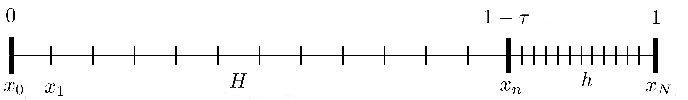
\includegraphics[width=0.85\linewidth]{figures/shmesh.pdf}
% %\\[2ex]
% %\includegraphics[width=0.5\linewidth]{figures/analytic_solution}
% \caption{Illustration of a one-dimensional Shishkin mesh.}
% \label{fig:back:shmesh1D}
% \caption{Illustration of a Shishkin mesh (top) and plot of the analytic
% solution of the problem \eqref{eq:back:1Dbvp} with $\epsilon=0.01$, $\omega=1$,
% $\beta=0$, $f(x)\equiv 1$, and $g_0=g_1=0$ (bottom). For $N=48$ the
% mesh transition point is $1-\tau_x=0.9226$.}\label{fig:back:shmesh1D}
%\end{figure}

In short, Shishkin meshes are formed by an overlapping union of piecewise
uniform meshes, with their respective sizes and mesh transition (or interface)
points adapted to the expected width of the boundary layers in the solution.
Suppose that an even integer $N\geq 4$ defining the number of intervals
constituting the Shishkin mesh is given, and suppose that the
\emph{mesh transition parameter}, $\tau_x$, fulfills
%
\begin{equation}\label{eq:back:tau_x}
\tau_x \equiv 2\frac{\epsilon}{\omega} \ln N \leq \frac{1}{2}.
\end{equation}
%
The inequality in \eqref{eq:back:tau_x} means that
%
\begin{equation}\label{eq:back:epsi}
\epsilon \leq \frac{\omega}{4 \ln N},
\end{equation}
%
which is a natural assumption since $\omega\gg \epsilon$, and the number of
mesh points usually is not exponentially large relative to $\epsilon$.
The \emph{mesh transition point} $1-\tau_x$ then will be close to $x=1$, and
the boundary layer will be contained in the (small) interval $[1-\tau_x, 1]$.
The idea of the Shishkin mesh discretization of the interval $[0,1]$ is to use
the same number of equidistantly distributed mesh points in each of the
subintervals $[0,1-\tau_x]$ and $[1-\tau_x,1]$ as can bee seen in
Figure~\ref{fig:back:shmesh1D}. Thus, if we denote
%
\begin{equation}\label{eq:back:nHh1D}
n\equiv \frac{N}{2},\quad H_x\equiv\frac{1-\tau_x}{n},\quad\text{and}\quad h_x\equiv \frac{\tau_x}{n},
\end{equation}
%
then the $N+1$ mesh points of the Shishkin mesh are given by
%
$$x_{i}\equiv iH_x, \quad i=0,\dots,n, \qquad x_{i}\equiv 1-(N-i)h_x, \quad i=n+1,\dots,N.$$
%
Here $x_0=0$ and $x_N=1$, so that the mesh consists of $N-1$ interior mesh
points, where the mesh point $x_n$ is exactly at the transition point
$1-\tau_x$. The ratio between the mesh sizes in the two subdomains is

\begin{align*}
\frac{h_{x}}{H_{x}} = \frac{\tau_x}{1-\tau_x} = \tau_x + \mathscr{O}(\tau_x^2),
\end{align*}
which is usually much less than $1$.

Any Shishkin mesh discretization naturally leads to a decomposition of the
given domain into overlapping subdomains. In our one-dimensional model problem
the domain is the interval $[0,1]$, and the overlapping subdomains are the
intervals $[0,1-\tau_x+h_x]$ and $[1-\tau_x-H_x,1]$.
The width of the overlap is $H_x+h_x=2/N$, and the mesh transition point
$x_n=1-\tau_x$ is the only mesh point in the overlap.
An illustration of a Shishkin mesh is shown in Figure~\ref{fig:back:shmesh1D},
and a plot of the (explicitly known) analytic solution of the problem
\eqref{eq:back:1Dbvp} with $\epsilon=0.03$, $\omega=1$, $\beta=0$,
$f(x)\equiv 1$, and $g_0=g_1=0$ is shown in Figure~\ref{fig:back:1D_analytic_sol}
 % \td{\textbf{fix}: Figure~\ref{fig:back:1D_analytic_sol} looks weird, chosen parameters make the transition point ``too far away"};
cf.~\cite[Example~3.1]{Sty05}. Choosing, for example, $N=48$ gives the mesh
transition point $1-\tau_x=0.7677$ (these parameters were chosen for
presentation purposes only, if we choose $\epsilon=0.01$ while keeping the
other parameters constant we obtain $1-\tau_x=0.9226$).

\begin{figure}[h!]
\centering
\begin{tikzpicture}[scale=0.43,declare function={ep=0.03;}]
%%%%% x-axis:
\draw[thick,-] (0,1) -- (11, 1);
\draw[thick,line width=1mm] (0,0.7)   -- (0, 1.3);
\draw[thick,line width=1mm] (11,0.7)  -- (11, 1.3);
\draw[thick,line width=1mm] (8.3,0.7) -- (8.3, 1.3);
\draw[dashed, color=gray] (8.3,0.7) -- (8.3, 10.7);
\foreach \i in {.83, 1.66, 2.49, 3.32, 4.15, 4.98, 5.81, 6.64, 7.47, 8.57, 8.84, 9.11, 9.34, 9.61, 9.88, 10.15, 10.42, 10.69}{
  \draw[thick,-] (\i,0.8) -- (\i, 1.2);
}
% \foreach \ii in {8.57,8.84,9.11,9.34,9.61,9.88,10.15,10.42,10.69}{
%   \draw[thick,-] (\ii,0.8) -- (\ii, 1.2);
% }
\node[below] at (0,0.7)  {$0$};
\node[below] at (8.3,0.7) {$1-\tau_x$};
\node[below] at (11,0.7) {$1$};
\draw[scale=11,domain=0:1,smooth,variable=\x, color=darkgray] plot ({\x},{.1+(\x - (exp(-(1-\x)/ep) - exp(-1/ep))/(1-exp(-1/ep)))});
\end{tikzpicture}
\caption{Analytic solution of problem \eqref{eq:back:1Dbvp} with $\epsilon=0.03$, $\omega=1$, $\beta=0$, $f(x)\equiv 1$, and $g_0=g_1=0$. For $N=48$ the mesh transition point is $1-\tau_x = 0.7677$.}
\label{fig:back:1D_analytic_sol}
\end{figure}
%
% \begin{figure}[h!]
% \centering
% \missingfigure[figwidth=6cm]{Solution to \eqref{eq:back:1Dbvp}.}
% \caption{Plot of the analytic solution of the problem \eqref{eq:back:1Dbvp} with $\epsilon=0.01$, $\omega=1$, $\beta=0$, $f(x)\equiv 1$, and $g_0=g_1=0$. For $N=48$ the mesh transition point is $1-\tau_x = 0.9226$.}
% \label{fig:back:1D_analytic_sol}
% \end{figure}

\subsection{Shishkin Mesh in 2D}
\label{back:convdiff:shihs2D}

In the case of two spacial dimensions, we can create various types of Shishkin
meshes depending on the number of outflow boundary layers in each coordinate
direction for a given problem. In the case of one boundary layer in one
direction and no layer in the other direction we will use a combination of a
regular discretization in the coordinate direction without a boundary layer
with a Shishkin mesh discretization in the coordinate direction with an
outflow boundary layer. In the other case we will use two Shishkin meshes, one
for each coordinate direction.
% \td{\textbf{write}: still need to mention in the previous subsections the ``well posedness" of the problem and its relation to the number of boundary layers}

\subsubsection{2.1.4.1. \ One Outflow Boundary Layer}
The simplest generalization of the Shishkin mesh for the case of two spacial
dimensions is to use a discretization approach that combines a regular mesh in
one coordinate direction (say $x$) with a Shishkin mesh discretization
in the other coordinate direction (say $y$).
%
\begin{figure}[h!]
\begin{minipage}[b]{0.4\textwidth}
\centering
\begin{tikzpicture}[scale = 0.4]
%%%% Rectangle:
\draw (0,0) rectangle (10, 10);
%%%% horizontal lines and $y$
\node[left] at (0,10) {$1$};
\draw (0,8) node[left] {$1-\tau_y$} -- (10,8);
\node[left] at (0,0) {$0$};
\node[below] at (0,0) {$0$};
\node[below] at (10,0) {$1$};
%%%% Black dots:
\draw[black,fill=black] (0,8) circle (0.5ex);
%%%% Tile labels
\node at (5,4) {$\Omega_1$};
\node at (5,9) {$\Omega_2$};
\end{tikzpicture}
\end{minipage}
  \hspace*{3em}
\begin{minipage}[b]{0.4\textwidth}
\centering
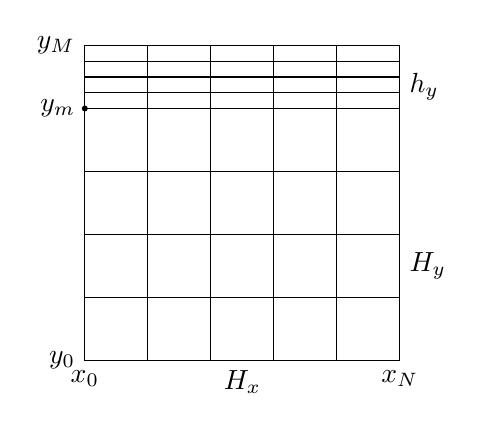
\begin{tikzpicture}[scale = 0.4]
%%%% Rectangle:
\draw (0,0) rectangle (10, 10);
%%%% horizontal lines and $y$
\node[left] at (0,10) {$y_M$};
\draw (0,9.5) -- (10,9.5);
\draw (0,9)  -- (10,9);
\draw (0,8) node[left] {$y_m$}  -- (10,8);
\draw (0,8.5)  -- (10,8.5);
\draw (0,6)  -- (10,6);
\draw (0,4)  -- (10,4);
\draw (0,2)  -- (10,2);
\node[left] at (0,0) {$y_0$};
%%%% vertical lines and $x$:
\node[below] at (0,0) {$x_0$};
\draw (2,0)  -- (2,10);
\draw (4,0)  -- (4,10);
\draw (6,0)  -- (6,10);
\draw (8,0)  -- (8,10);
\node[below] at (10,0) {$x_N$};
%%%% Black dots:
\draw[black,fill=black] (0,8) circle (0.5ex);
%%%% Tile labels
\draw (5,0) node[below] {$H_x$};
\draw (10,3) node[right] {$H_y$};
\draw (10,8.7) node[right] {$h_y$};
\end{tikzpicture}
\end{minipage}
%\includegraphics[width=0.9\linewidth]{figures/simpleShish2D3.pdf}
\caption{Division of the domain and Shishkin mesh for equation \eqref{eq:back:nDbvp} with one outflow exponential layer.}
\label{fig:back:shmesh2Da}
\end{figure}

Given now two even positive integers $N\geq 4$ and $M\geq 4$ that denote the
number of mesh intervals used in each coordinate direction, we let the
transition parameter $\tau_y$ that will be used to specify where the mesh
changes from coarse to fine in the $y$-direction, be defined by
%
\begin{equation}\label{eq:back:tau_y}
\tau_y~\equiv~\min\left\{\frac{1}{2},2\frac{\epsilon}{\omega_y}  \ln M\right\}.
\end{equation}
%
Since we assume $\omega_y\gg \epsilon$ (or equivalently that
$\epsilon \leq CM^{-1}$), we will have
$\tau_y~=~2\frac{\epsilon}{\omega_y}\ln M~\ll~1$,
so that in this case the \emph{mesh transition point} $1-\tau_y$ will be very
close to the boundary $y=1$. By assuming that the parameters of the problem,
i.e. $\epsilon, \om, \beta$, $f$, and  $g$, are chosen so that the solution
$u(x,y)$ has one boundary layer at $y=1$. In particular, this is achieved by
assuming that $\om=[0,\omega_y]^T$, and $\omega_y>0$. The use of this Shishkin
mesh discretization scheme will divide the domain $\Omega$ into two overlapping
subdomains, $\overline{\Omega}=\Omega_{1}\cup\Omega_{2}$, where
%
$$
\Omega_{1}=[0,1]\times[0,1-\tau_y],\quad\Omega_{2}=[0,1]\times[1-\tau_y,1].
$$
%
This subdivision is shown in the left side of Figure~\ref{fig:back:shmesh2Da}.
% Each subdomain is then decomposed into $N/2\times N/2$ rectangles with $N/2$ interior nodes in each subdomain.
%

Let $m\equiv \frac{M}{2}$, if we denote by $H_x$ the mesh width in the $x$-
direction and by $h_y$ and $H_y$ the mesh widths inside and outside the
boundary layer in the $y$-direction, i.e.,
%
\begin{equation}\label{eq:back:Hh2D}
H_x\equiv\frac{ 1}{N},
\;\;\quad
h_y\equiv\frac{\tau_y}{m},
\;\;\quad\mbox{and}\;\;\quad
H_y\equiv\frac{( 1-\tau_y)}{m},
 \end{equation}
%\begin{equation}\label{eq:back:tau}
%h_i=
%\begin{cases}h_1\equiv\frac{2( 1-\tau_x)}{N} &\mbox{for}\;\; i=0,\ldots,n \\
%h_2\equiv\frac{\tau_x}{N} &\mbox{for}\;\; i=n+1,\ldots,N. \end{cases}
%\quad
%%\text{and}\quad
%k_i=
%\begin{cases}k_1\equiv\frac{2( 1-\tau_y)}{N} &\mbox{for}\;\; i=0,\ldots,n \\
%h_2\equiv\frac{\tau_y}{N} &\mbox{for}\;\; i=n+1,\ldots,N. \end{cases}
%\end{equation}
%,\quad H\equiv\frac{1-\tau}{n},\quad h\equiv \frac{\tau}{n},
%
then the $(N+1)\times(M+1)$ nodes of the Shishkin mesh are given by
\[
\Omega_D=\{(x_i,y_j)\in\overline{\Omega}:i=0,\ldots,N, j=0,\ldots,M\},
\]
where
%
\begin{equation}\label{eq:back:shishmeshnodes}
x_i\equiv iH_x,\;\mbox{for}\;\; i=0,\ldots,N,
\quad \mbox{ and } \quad
y_j\equiv
\begin{cases} jH_y &\mbox{for}\;\; j=0,\ldots,m, \\
1-(N-j)h_y &\mbox{for}\;\; j=m+1,\ldots,M. \end{cases}
\end{equation}
%
%$$x_{i}\equiv iH, \quad i=0,\dots,n, \qquad x_{i}\equiv 1-(N-i)h, \quad i=n+1,\dots,N.$$
%
The mesh is constructed by drawing lines parallel to the coordinate axes
through these mesh points; see the right side of
Figure~\ref{fig:back:shmesh2Da}. Here $x_0=0$, $y_0=0$ and $x_N=1$, $y_M=1$
so that the mesh consists of $N-1$ interior nodes in each direction and where
the node $y_m$ is exactly at the transition point $1-\tau_y$ in the $y$-
direction. In contrast to the one-dimensional case where the overlapping
subdomains intersect in exactly one grid point, in this two-dimensional case
we have a whole row of grid points in common. The $N-1$  nodes with vertical
coordinate equal to $y_n=1-\tau_y$ are the grid points in the overlap. It is
clear that the mesh widths on $\Omega_{1}$ satisfy
$1/N\leq H_x,\, H_y\leq 2/M$, so the mesh is coarse in this domain. On the
other hand, $h_y$ is $\mathscr{O}(\epsilon M^{-1}\log(M))$, so on $\Omega_2$
the mesh is coarse in the $x$ direction and fine in the $y$ direction. The
ratio between the different mesh sizes in the $y$ direction is
%
\[\frac{h_y}{H_y}=\frac{\tau_y}{1-\tau_y}=\tau_y+\mathscr{O}(\tau_y^2) \ll 1.\]
%


\begin{example}
We consider the BVP \eqref{eq:back:nDbvp} defined on $\Omega=(0,1)\times(0,1)\in\mathbb{R}^{2}$ with $\beta=0$, $f=0$ and boundary conditions determined by the function
%
\begin{equation}\label{analytic_solution}
u(x,y)=(2x-1)\left(\frac{1-e^{(2y-2)/\epsilon}}{1-e^{-2/\epsilon}}\right).
\end{equation}
%
A three-dimensional rendering of the analytic solution to this problem is
shown in Figure~\ref{fig:back:2D_analytic_sol} for the case $\epsilon=0.01$.
In most parts of the domain $\Omega$, the values of the solution $u(x,y)$
closely resemble the ones given by the \emph{inflow boundary} condition
$u(x,0)=2x-1$, except in a vicinity of the \emph{outflow boundary} where they
abruptly change to the constant values $u(x,1)~=~0$. The boundary conditions at
$x=0$ and $x=1$ satisfy $u(0,y)\approx-1$ and $u(1,y)\approx 1$ respectively
(see \cite[Example 6.1.1]{ElmSilWat14} where a similar problem is presented)
and its values also change drastically as they approach the outflow
boundary, where they change from $\approx-1$ or $\approx 1$ to $0$.
The portion of the domain where these changes occur is proportional to
$\epsilon$ and it is determined by the function $e^{(2-2y)/\epsilon}$, thus,
when small enough values of $\epsilon$ are chosen, the changes in the function
$u$ occur abruptly enough and in a portion of the domain that is small enough
so that the solution of \eqref{eq:back:nDbvp} presents an exponential boundary
layer in this particular region of the domain.
%
\begin{figure}[h!]
\begin{minipage}[t]{0.5\linewidth}
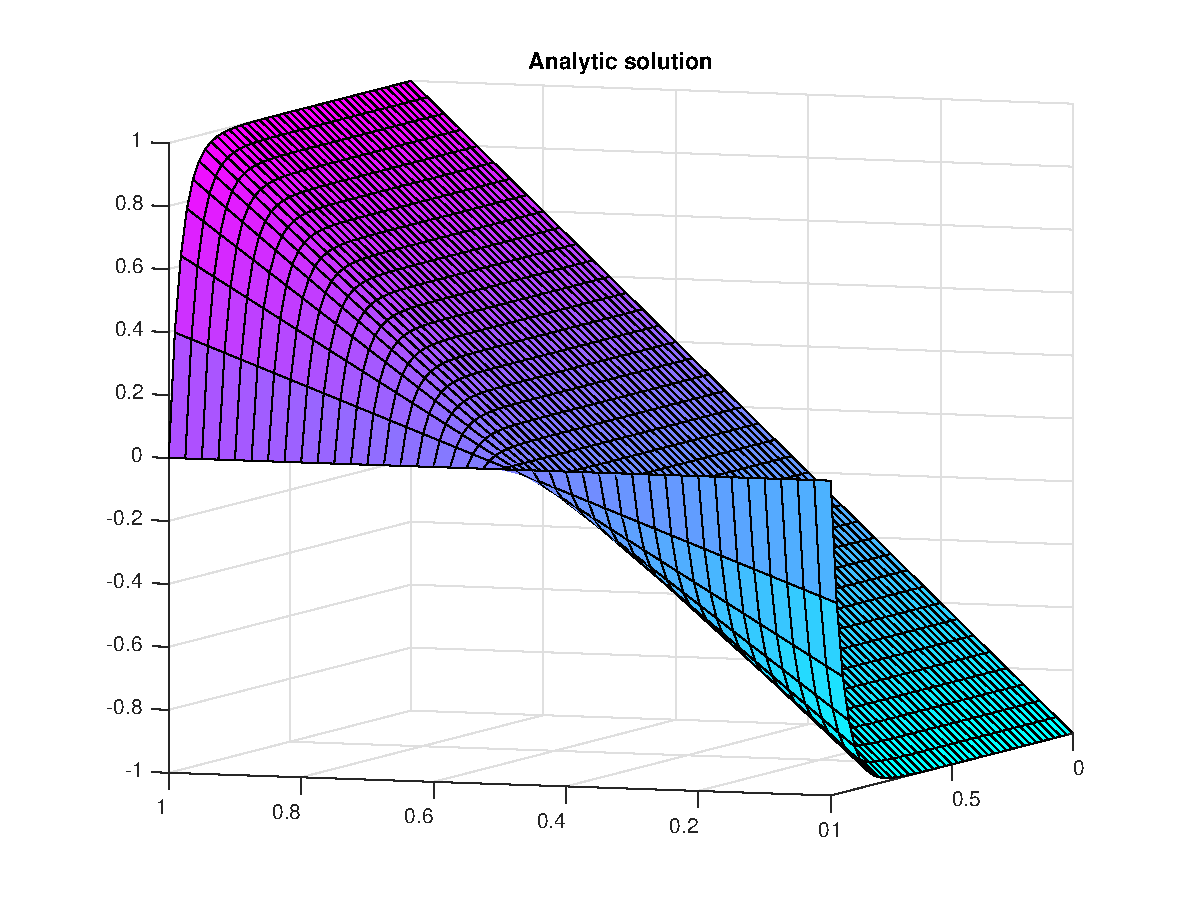
\includegraphics[width=0.83\linewidth]{figures/analytic_sol_new}
\end{minipage}
%
\begin{minipage}[t]{0.5\linewidth}
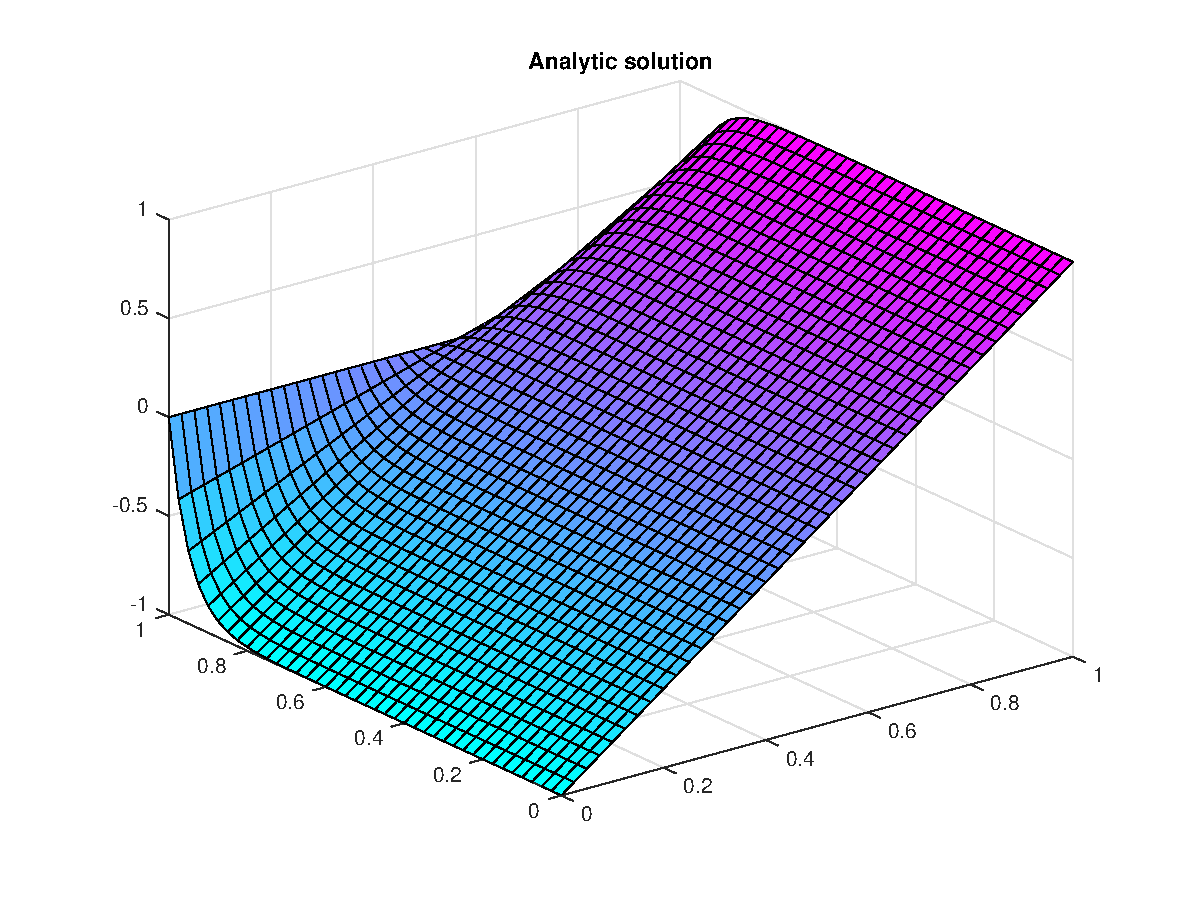
\includegraphics[width=0.83\linewidth]{figures/analytic_sol_new2b}
\end{minipage}
\caption{Three-dimensional surface plot of the analytic solution of
\eqref{eq:back:nDbvp} with $n=2$, $\omega_x,\beta=0$ and $\epsilon=10^{-1}$ for two different viewing angles.}
\label{fig:back:2D_analytic_sol}
\end{figure}

This will be the main example used in future chapters to exemplify the theoretical results obtained for two-dimensional problems.
\end{example}

\subsubsection{2.1.4.2. \ Two Outflow Boundary Layers}
In the case of two outflow boundaries, we can now use a one dimensional Shishkin mesh in each coordinate direction.
Again, given two even positive integers $N\geq 4$ and $M\geq 4$ that denote the
number of mesh intervals used in each coordinate direction, let the transition
parameters $\tau_x$ and $\tau_y$, that will be used to specify where the mesh
changes from coarse to fine, be defined by
%
\begin{equation}\label{eq:back:tau_xy}
\tau_x \equiv \min\left\{\frac12,2\frac{\epsilon}{\omega_x}  \ln N\right\}\quad\text{ and }\quad\tau_y \equiv \min\left\{\frac12,2\frac{\epsilon}{\omega_y} \ln M\right\}.
\end{equation}
%
Once again, since we assume $\omega_x,\omega_y\gg \epsilon$, we will usually
have $\tau_x=2\frac{\epsilon}{\omega_x}  \ln N\ll 1$ and
$\tau_y=2\frac{\epsilon}{\omega_y} \ln M\ll 1$, so that in both spacial
directions the \emph{mesh transition points} $1-\tau_x$ and $1-\tau_y$ will be
located very close to the boundary with $x=1$ in the $x$-direction and very
close to the boundary with $y=1$ in the $y$-direction.
%Otherwise, the analysis can be carried out using standard techniques.

In the case of this discretization scheme the domain $\Omega$ is divided into
four overlapping subdomains, where
$\overline{\Omega}=\Omega_{1}\cup\Omega_{2}\cup\Omega_{3}\cup\Omega_{4}$.
That is, by again letting $n\equiv \frac{N}{2}$ and $m\equiv \frac{M}{2}$, the
mesh division divides $\Omega$ into a set of 4 subdomains, each of
them consisting of $n\times m$ rectangles giving $nm$ interior nodes in each
subdomain. This subdivision is shown on the left side of
Figure~\ref{fig:back:shmesh2Db}.
%
\begin{figure}[h!]
% \includegraphics[width=0.8\linewidth]{figures/Shish2D}
\hspace*{-2em}
\begin{minipage}[b]{0.5\textwidth}
\centering
\begin{tikzpicture}[scale = 0.4]
%%%% Rectangle:
\draw (0,0) rectangle (10, 10);
%%%% horizontal lines and $y$
\node[left] at (0,10) {$1$};
\draw (0,8) node[left] {$1-\tau_y$} -- (10,8);
\node[left] at (0,0) {$0$};
\node[below] at (0,0) {$0$};
\node[below] at (10,0) {$1$};
\draw (8,0) node[below] {$1-\tau_x$} -- (8,10);

%%%% Black dots:
\draw[black,fill=black] (0,8) circle (0.5ex);
\draw[black,fill=black] (8,8) circle (0.5ex);
\draw[black,fill=black] (8,0) circle (0.5ex);
%%%% Tile labels
\node at (4,4) {$\Omega_x$};
\node at (9,4) {$\Omega_2$};
\node at (4,9) {$\Omega_3$};
\node at (9,9) {$\Omega_4$};
\end{tikzpicture}
\end{minipage}
%
\hspace*{1em}
%
\begin{minipage}[b]{0.5\textwidth}
\centering
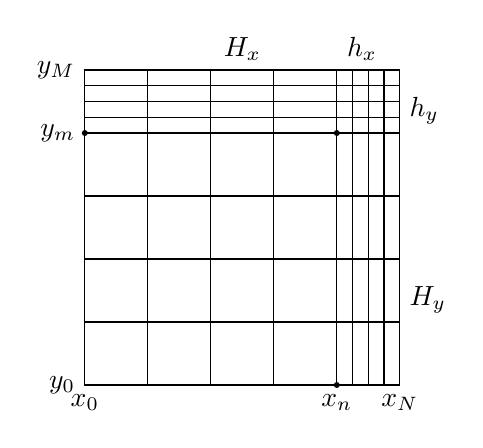
\begin{tikzpicture}[scale = 0.4]

%%%% Rectangle:
\draw (0,0) rectangle (10, 10);

%%%% horizontal lines and $y$
\foreach \point in {2,4,6,8,8.5,9,9.5}
\draw (0,\point) -- (10,\point);
\node[left] at (0,10) {$y_M$};
\node[left] at (0,8) {$y_m$};
\node[left] at (0,0) {$y_0$};

%%%% vertical lines and $x$:
\foreach \point in {2,4,6,8,8.5,9,9.5}
\draw (\point,0) -- (\point,10);
\node[below] at (0,0) {$x_0$};
\node[below] at (8,0) {$x_n$};
\node[below] at (10,0) {$x_N$};

%%%% Black dots:
\draw[black,fill=black] (0,8) circle (0.5ex);
\draw[black,fill=black] (8,8) circle (0.5ex);
\draw[black,fill=black] (8,0) circle (0.5ex);

%%%% Tile labels
\draw (5,10) node[above] {$H_x$};
\draw (8.8,10) node[above] {$h_x$};
\draw (10,2.7) node[right] {$H_y$};
\draw (10,8.7) node[right] {$h_y$};
\end{tikzpicture}
\end{minipage}
%\includegraphics[width=0.9\linewidth]{figures/simpleShish2D3.pdf}
\caption{Division of the domain and Shishkin mesh for equation
\eqref{eq:back:nDbvp} with two outflow exponential layers.}
\label{fig:back:shmesh2Db}
\end{figure}

If we denote the mesh widths outside and inside the respective boundary layers
by $H_x$, $h_x$ and $H_y$, $h_y$, i.e.,
%
\begin{eqnarray*}
H_{x}\equiv\frac{( 1-\tau_x)}{n}, \qquad
h_{x}\equiv\frac{\tau_x}{n},\qquad
H_{y}\equiv\frac{( 1-\tau_y)}{m},\qquad
h_{y}\equiv\frac{\tau_y}{m},
\end{eqnarray*}
then the four overlapping subdomains are given by
%
\begin{eqnarray}\label{eq:back:subdomains_a}
\Omega_{1}=&[0,1-\tau_x+h_x)\times[0,1-\tau_y+h_y),\qquad\Omega_{2}&=(1-\tau_x-H_x,1]\times[0,1-\tau_y+h_x),\nonumber\\
\Omega_{3}=&[0,1-\tau_x+h_x)\times(1-\tau_y-H_y,1],\qquad\Omega_{4}&=(1-\tau_x-H_x,1]\times(1-\tau_y-H_y,1],\nonumber\\
\end{eqnarray}
%
the $(N+1)\times(M+1)$ nodes of the two-dimensional Shishkin mesh are now given
by
$$
\Omega_D=\{(x_i,y_j)\in\overline{\Omega}:i=0,\ldots,N, j=0,\ldots,M\},
$$
where
%
$$
%\hspace*{-4em}
x_i\equiv
\begin{cases} iH_x &\mbox{for}\;\; i=0,\ldots,n \\
1-(N-i)h_x &\mbox{for}\;\; i=n+1,\ldots,N, \end{cases},
$$
%\quad
and
$$
y_j\equiv
\begin{cases} jH_y &\mbox{for}\;\; j=0,\ldots,m \\
1-(M-j)h_y &\mbox{for}\;\; j=m+1,\ldots,M. \end{cases}
$$
%
The mesh is constructed by drawing lines parallel to the coordinate axes
through these mesh points, i.e., the mesh is obtained by a tensor product of
two one-dimensional piecewise uniform meshes; see the right side of
Figure~\ref{fig:back:shmesh2Db}. Here $x_0=0$, $y_0=0$ and $x_N=1$, $y_M=1$
so that the mesh consists of $N-1$ and $M-1$ interior nodes in each respective
direction, where the node $x_n$ is exactly at the transition point $1-\tau_x$
and the node $y_n$ is exactly at the transition point $1-\tau_y$.
It is clear that the mesh widths on $\Omega_{1}$ satisfy
$1/N\leq H_x\leq 2/N$ and $1/M\leq H_y\leq 2/M$, so the mesh is coarse in this
domain. On the other hand, $h_x$ and $h_y$ are
$\mathscr{O}(\epsilon N^{-1}\log(N))$ and
$\mathscr{O}(\epsilon M^{-1}\log(M))$ respectively,
so the mesh is very fine on $\Omega_{4}$. On $\Omega_{2}$ and $\Omega_{3}$, the
mesh is coarse in one direction and fine in the other direction. The ratio
between the different mesh sizes in the $x$-coordinate direction is again
%
\[\frac{h_x}{H_x}=\frac{\tau_x}{1-\tau_x}=\tau_x+\mathscr{O}(\tau_x^2) \ll 1.\]
%
and similarly for the ratio $\frac{h_y}{H_y}$.
% \td{\textbf{add}: need to add a picture of a solution for a 2D boundary-layer problem with 2 layers (double glazing problem maybe?)}

\subsection{Approximation of BVPs}
\label{back:convdiff:BVPapprox}
In the most general setting, in order to find a finite difference
representation of a BVP, both the PDE and the boundary conditions need to be
replaced with a suitable approximation. Here, the approximation process will be
illustrated through the Dirichlet problem of the convection diffusion
equation posed on the square domain $\Omega=(0,1)\times(0,1)$.

We first denote the internal grid points where the equation will be
approximated~by
\[
\Omega_D=\{(x_i,y_j);i=1,\ldots,N-1;\;j=1,\ldots,M-1\},
\]
and denote the grid points on the boundary by $\partial\Omega_D$ and the
entire grid by $\overline{\Omega}_D=\Omega_D\cup\partial\Omega_D$.
Since boundary conditions of Dirichlet-type are exact in the
boundary nodes, an approximation of the boundary conditions is not needed and
we can focus our attention on the approximation of the PDE. We proceed to
evaluate the PDE of our two-dimensional BVP~\eqref{eq:back:nDbvp} at the
internal grid points of the mesh to obtain
%
\begin{equation}\label{eq:back:2Dpde}
-\epsilon \Delta u(x_i,y_j) + \omega(x_i,y_j)\cdot \nabla u(x_i,y_j) + \beta(x_i,y_j) u(x_i,y_j) = f(x_i,y_j).
\end{equation}
%
Using the standard finite difference operators
(see Table~\ref{tab:back:findiff} or e.g., \cite[\S~4]{Sty05})
to represent the first and second derivative terms and using the notation
$\omega_{ij}=\omega(x_i,y_j)$, $\beta_{ij}=\beta(x_i,y_j)$, $f_{ij}=f(x_i,y_j)$, etc., leads to the the upwind scheme approximation
%
\begin{equation}\label{eq:back:2DpdeO}
-\epsilon \left( h_{x_{i}}^{-2}\delta^2_x u_{ij} + h_{y_{j}}^{-2}\delta^2_y u_{ij}\right) + \omega^x_{ij} h_{x_{i}}^{-1}\Delta^{-}_{x}u_{ij} + \omega^y_{ij} h_{y_{j}}^{-1}\Delta^{-}_{y}u_{ij} + \beta_{ij} u_{ij} + \mathscr{O}(h_{x_{i}}) + \mathscr{O}(h_{y_{j}}) = f_{ij}.
\end{equation}
%
This equation is satisfied exactly by the solution to the continuous BVP.
By neglecting the higher order terms, equation~\eqref{eq:back:2DpdeO} will no
longer be satisfied by $u$ but by a grid function $u^D$ which we hope will be
close to the solution $u$. The finite difference equations that approximate
the PDE are obtained by discarding the remainder terms to yield, for each
point $(x_i,y_i)\in\Omega_D$, an algebraic equation of the form
\begin{equation}\label{eq:back:2Dpde_disc}
-\epsilon \left( h_{x_{i}}^{-2}\delta^2_x + h_{y_{j}}^{-2}\delta^2_y \right)u_{ij} + \omega^x_{ij} h_{x_{i}}^{-1}\Delta^{-}_{x}u_{ij} + \omega^y_{ij} h_{y_{j}}^{-1}\Delta^{-}_{y}u_{ij} + \beta_{ij} u_{ij}  = f_{ij}.
\end{equation}
Since the values of the grid function are known on the boundary
$\partial\Omega_D$, then equation \eqref{eq:back:2Dpde_disc} gives
$(N-1)\times(M-1)$ linear equations to determine the unknown values of the
grid function on $\Omega_D$.

By repeating this process for each point $(x_i,y_i)\in\Omega_D$
%$(x_i,y_j)$ for $i=1,\ldots,N-1$, $j=1,\ldots,M-1$
we can obtain a finite difference approximation, $\mathscr{A}^D$, of the
differential operator~$\mathscr{A}$ (defined in \eqref{eq:back:ellipticPDE}):
%
% \A\u\equiv-\epsilon h_{x}^{-1}\delta^2 u^N_m + \omega_m h_x^{-1}\Delta^{-}u^N_m +\beta_m u^N_m,\quad m=1,2,\ldots,N-1.
%
% \A u^{D}\equiv-\epsilon \left( h_{m}^{-1}\delta^2_x u^D_{ij} + h_{m}^{-1}\delta^2_y
% u^D_{ij}\right) + \omega_x h_m^{-1}D^{-}_{x}u^D_{ij} + \omega_y h_m^{-1}D^{-}_{y}u^D_{ij} + \beta_{ij} u^D_{ij},\quad \substack{i=1,\ldots,N-1,\\ j=1,\ldots,M-1}
\begin{equation}\label{eq:back:2DdiscrOp}
\mathscr{A}^D \equiv-\epsilon \left( h_{x_{i}}^{-2}\delta^2_x + h_{y_{j}}^{-2}\delta^2_y\right) + \omega^x_{ij} h_{x_{i}}^{-1}\Delta^{-}_{x} +
\omega^y_{ij} h_{y_{j}}^{-1}\Delta^{-}_{y} + \beta_{ij},\quad \substack{i=1,\ldots,N-1,\\ j=1,\ldots,M-1},
\end{equation}
%
and we can thus write the (upwind) finite difference discretization of our BVP as:
%
\begin{equation}\label{eq:back:2DbvpD}
\begin{cases}
%\A u^{D}_{i,j} =
\mathscr{A}^Du^D_{ij}\equiv-\epsilon \left( h_{x_{i}}^{-2}\delta^2_x +
h_{y_{j}}^{-2}\delta^2_y\right) u^D_{ij} + \omega_x h_{x_{i}}^{-1}\Delta^{-}_{x} u^D_{ij} + \omega_y h_{y_{j}}^{-1}\Delta^{-}_{y}u^D_{ij} + \beta_{ij}
u^D_{ij}  = f_{ij},
& \text{ in } \Omega^D,\\
%\substack{i=1,\ldots,N-1,\\ j=1,\ldots,M-1},\\
%-\epsilon h_{x}^{-1}\delta^2 u^D_i + \omega_m h_x^{-1}\Delta^{-}u^D_i +\beta_m u^D_i = f_m, & i=1,\ldots,N,\\
\hspace{9.35cm} \mathscr{B}^Du^D_{ij}\equiv u^D_{ij} = g_{ij}, &
\text{ on } \partial\Omega^D,\\
%\substack{i=0,N \\ j=0,M},
%\hspace{10cm} u^D_{i,j}|_{\partial \Omega} = g, & \quad \substack{i=0,N \\ j=0,M},
\end{cases}
\end{equation}
%That is, a finite difference operator $\A$
%($\mathscr{A}^{N}$the superscript $N$ acting as a reminder that it involves a grid with a total of $N$ intervals)
% that represents the discretized differential equation \eqref{eq:back:tau_xy} is defined by\td{get rid of the fraction line in the following equation}:
%
% Since the values of the grid function are known on the boundary $\partial\Omega^D$, equation \eqref{eq:back:2DbvpD} yields $(N-1)\times(M-1)$ linear equations to determine the unknown values of the grid function on $\Omega^D$.
% By letting $\f$ represent the corresponding source term (its $(i,j)$-th
% component in this case being $\f_{ij}=f_{ij}$), we can write equation
% \eqref{eq:back:2Dpde} concisely as $\A\u=\f$.
The $(N-1)\times(M-1)$ finite difference equations approximating the BVP
\eqref{eq:back:ellipticBVP} can be written compactly as
$\mathcal{A}^Du^D=\mathcal{F}^D$ where
\begin{equation}
\mathcal{A}^{D}u^D =
\begin{cases}
\mathscr{A}^{D}u^{D} & \text{ in } \Omega_D,\\
\mathscr{B}^{D}u^{D} & \text{ on } \partial\Omega_D,
\end{cases}
%\end{equation}
\;\text{
 and
}\;
%\begin{equation}
\mathcal{F}^D=
\begin{cases}
f   & \text{ in } \Omega_D,\\
g   & \text{ on } \partial\Omega_D.
\end{cases}
\label{eq:back:2DconvdiffD}
\end{equation}
% In the next section we will see how we can write the discrete BVP
% \eqref{eq:back:2DconvdiffD} as a matrix-vector equation of the form \eqref{eq:int:linsys}.

%
\subsection{The Shishkin Mesh Discretization of Convection-Diffusion BVPs}
\label{back:ModProb}

We can apply the concepts of the previous section to problems where the domain
is $n$-dimensional. In this work we present the results for $n=1,2$, and we
direct the reader to \cite[\S~6.2]{GriDolSil15} for a detailed description
of the case where $n=1$.

\subsubsection{2.1.6.1. \ 1D Problems}
We first consider the one-dimensional convection-diffusion boundary value
problem with constant coefficients and Dirichlet boundary conditions given by
\eqref{eq:back:1Dbvp} and proceed to apply the finite difference procedure
described in Section \ref{back:convdiff:findiff} on the one-dimensional
Shishkin mesh presented in Section \ref{back:convdiff:shihs1D} and shown in
Figure \ref{fig:back:shmesh1D}.

% The first derivative of $u$ at the point $x_i$ approximated by the standard
% upwind finite difference operator (see Section \ref{back:convdiff:findiff}) is
% given by
% \begin{equation*}
% %\frac{\partial u(x_i)}{\partial x}
% u'(x_i)\approx
% %(\Delta x)^{-1}D^{-}_{x} u_{i}^D = (\Delta x)^{-1}(u_{i}^D-u_{i-1}^{N})=
% \frac{u_i^D-u_{i-1}^{N}}{h_i},
% \end{equation*}
% and using the central finite difference operator we obtain
% \begin{equation*}\label{eq:firstcen}
% %\frac{\partial u(x_i)}{\partial x}
% u'(x_i)\approx %(\Delta x)^{-1} D^{0}_{x} u_{i}^D =(\Delta x)^{-1}(u_{i+1}^D-u_{i-1}^{N})=
% \frac{u_{i+1}^D-u_{i-1}^{N}}{(h_i+h_{i+1})}.
% \end{equation*}
% The second derivative can be approximated by
% \begin{equation*}
% %\frac{\partial u(x_i)}{\partial x^2}
% u''(x_i)\approx %\delta^{2}_{x} u_{i}^D\; =\;
% \frac{2 u_{i-1}^D}{(h_{i} + h_{i+1}) h_{i+1}}- \frac{2u_{i}^D}{h_{i} h_{i+1}} + \frac{2 u_{i+1}^D}{(h_{i} + h_{i+1}) h_{i+1}}.
% \end{equation*}
Applying the discrete operators given in Table~\ref{tab:back:findiff} on the
nodes of the Shishkin mesh, where $h_i=H_x$ for $i=1,\ldots,n$ and $h_i=h_{x}$
for $i=n+1,\ldots,N-1$, we obtain for the upwind scheme:
%\td{\textbf{fix:}is it $D^{0}$ or $\Delta^{0}$?}
\begin{equation}
\Delta^{-}_{x} u_{i}^D\; =\;
\begin{cases}
\frac{1}{H_x}\left(u_{i}^D-u_{i-1}^D\right) & \mbox{for}\;\; i=1,\ldots, n, \\
\frac{1}{h_x}\left(u_{i}^D-u_{i-1}^D\right) & \mbox{for}\;\; i={n+1},\ldots, N-1,
\end{cases}
\end{equation}
and for the central finite difference scheme we obtain
\begin{equation}
\Delta^{0}_{x} u_{i}^D\; =\;
\begin{cases}
\frac{1}{2H_x}\left(u_{i+1}^D-u_{i-1}^D\right) &
\mbox{for}\;\; i=1,\ldots, {n-1},\\
\frac{1}{h_x+H_x}\left(u_{i+1}^D-u_{i-1}^D\right)  &
\mbox{for}\;\; i=n,\\
\frac{1}{2h_x}\left(u_{i+1}^D-u_{i-1}^D\right)  &
\mbox{for}\;\;i={n+1},\ldots, {N-1}.
\end{cases}
\end{equation}
For the second derivatives, we obtain
\begin{equation}
\label{eq:back:second}
\delta^{2}_{x} u_{i}^D\; =\;
\begin{cases}
\frac{1}{H_x^2}\left(u_{i-1}^D - 2u_{i}^D + u_{i+1}^D\right) &
\mbox{for}\;\; i=1,\ldots, {n-1},\\
\frac{2u_{i-1}^D}{(H_x+h_x)H_x} - \frac{2u_{i}^D}{H_xh_x} + \frac{2u_{i+1}^D}{(H_x+h_x)h_x} &
\mbox{for}\;\; i=n,\\
\frac{1}{h_x^2}\left(u_{i-1}^D - 2u_{i}^D + u_{i+1}^D\right) &
\mbox{for}\;\;i={n+1},\ldots, {N-1}.
\end{cases}
\end{equation}

% Considering the homogeneous boundary conditions $u_0 = u_1 = 0$ and letting
% $\omega(x)=\omega>0$, and $\beta(x) = \beta>0$ be constant along the domain,
% the finite difference scheme applied to the differential equation in \eqref{eq:1D:bvp} on
% the Shishkin mesh is then given~by
% \begin{equation}\label{eq:1DdiscrOp}
% %\Au^D_m\equiv
% -\epsilon \delta_x^2 u^D_i + \omega \Delta^{-/0}_{x}u^D_i +\beta_i u^D_i= f_i,\quad i=1,2,\ldots,N-1\equiv M.
% \end{equation}
Thus, by including the boundary conditions and letting $\omega(x)=\omega_x>0$
and $\beta(x) = \beta > 0$ be constant along the domain, the finite difference
scheme applied to the continuous problem \eqref{eq:1D:bvp} results in the
discrete version of our model problem:
% consists of the
% following discretization of the one-dimensional convection-diffusion boundary
% value problem with constant coefficients and Dirichlet boundary conditions:
%
\begin{equation}
\label{eq:back:1DbvpDiscr}
\begin{cases}
%\A\u\equiv
-\epsilon \delta^2 u^D_i + \omega_i \Delta^{-/0}u^D_i +\beta_i u^D_i = f_i, & i=1,\ldots,N-1,\\
\;\;u^D_0=g_0,\;\;u^D_N=g_1, &
\end{cases}
\end{equation}

By collecting all equations for $i=1,\ldots,N-1$, both finite difference
schemes yield a linear algebraic system \eqref{eq:1D:linsys} with the
tridiagonal and nonsymmetric $(N-1)\times (N-1)$ coefficient matrix given by:
%
\begin{equation}
\label{eq:back:1Dmatrix}
\A=\left[
  \begin{array}{cccc|c|cccc}
     \entryvC &\entryvE    &  &  &  &  &  &  &  \\
     \entryvW &\ddots &\ddots  &  &  &  &  &  &  \\
     &  \ddots& \ddots &  \entryvE   &  &  &  &  &  \\
     &  &\entryvW & \entryvC  & \entryvE   &  &  &  &  \\ \hline
     &  &  & \entryzW  & \entryzC  & \entryzE  &  &  &  \\ \hline
     &  &  &  & \entrywW  & \entrywC  & \entrywE  &  &  \\
     &  &  &  &  & \entrywW  & \ddots & \ddots &  \\
     &  &  &  &  &  & \ddots & \ddots & \entrywE  \\
     &  &  &  &  &  &  & \entrywW  & \entrywC  \\
  \end{array}
\right].%\;\in\;{\mathbb R}^{(N-1)\times (N-1)}.
\end{equation}
%
For the upwind scheme, the entries of $\A$ are given by
%
\begin{align}
    &\entryvW  =  -\frac{\epsilon}{H^{2}} - \frac{\omega_x}{H},&
    &\entryvC  =  \frac{2\epsilon}{H^{2}} + \frac{\omega_x}{H}+\beta, &
    &\entryvE   =  -\frac{\epsilon}{H^{2}}, \nonumber \\
    &\entryzW  =  -\frac{2\epsilon}{H(H+h)} - \frac{\omega_x}{H},&
    &\entryzC  =  \frac{2\epsilon}{hH} + \frac{\omega_x}{H}+\beta,&
    &\entryzE  =  -\frac{2\epsilon}{h(H+h)}, \label{eq:back:upwind} \\
    &\entrywW  =  -\frac{\epsilon}{h^{2}} - \frac{\omega_x}{h},&
    &\entrywC  =  \frac{2\epsilon}{h^{2}} + \frac{\omega_x}{h}+\beta,&
    &\entrywE  =  -\frac{\epsilon}{h^{2}}, \nonumber
\end{align}
%
and for the central difference scheme by
%
\begin{align}
    &\entryvW  =  -\frac{\epsilon}{H^{2}} - \frac{\omega_x}{2H},&
    &\entryvC  =  \frac{2\epsilon}{H^{2}} + \beta, &
    &\entryvE  =  -\frac{\epsilon}{H^{2}}+\frac{\omega_x}{2H}, \nonumber \\
    &\entryzW  =  -\frac{2\epsilon}{H(H+h)} -\frac{\omega_x}{h+H},&
    &\entryzC  =  \frac{2\epsilon}{hH} + \beta,&
    &\entryzE  =  -\frac{2\epsilon}{h(H+h)}+\frac{\omega_x}{h+H}, \label{eq:back:central} \\
    &\entrywW  =  -\frac{\epsilon}{h^{2}} - \frac{\omega_x}{2h},&
    &\entrywC  =  \frac{2\epsilon}{h^{2}} +\beta,&
    &\entrywE  =  -\frac{\epsilon}{h^{2}}+ \frac{\omega_x}{2h}. \nonumber
\end{align}

% Moreover, we can express the system matrix \eqref{eq:back:1Dmatrix} using the
% standard finite difference matrices, see,~\cite[Section~2]{PalSim15}. Consider
% the following proposition:
% %
% \begin{prop}
% Let $x_i\in\Omega^D=\{x_i\in\overline{\Omega}:i=0,\ldots,N;\},$
% be the $N+1$ nodes of the Shishkin mesh. Then the upwind finite
% difference discretization of the differential operator in \eqref{eq:1D:bvp}
% leads to the following discrete operator:
% \begin{equation}\label{eq:1Dkronrep}
% A =
% \epsilon (D_{xx}T+e_{n}v_{x}^T) + \omega_xD_xB_{up/cd} + \beta I,
% \end{equation}
% where
% \begin{eqnarray}
% T      &=& \mathrm{tridiag}(1,-2,1) \in \mathbb{R}^{M\times M},\nonumber\\
% B_{up} &=& \mathrm{tridiag}(-1,1,0) \in \mathbb{R}^{M\times M},\nonumber\\
% B_{cd} &=& \mathrm{tridiag}(-1,1,-1)\in \mathbb{R}^{M\times M},\nonumber\\
% D_{x}  &=& \mathrm{diag}\left(\underbrace{H_x^{-1},\dots,
%            H_x^{-1}}_{n},\underbrace{h_x^{-1},\ldots,
%            h_x^{-1}}_{m}\right)\in\mathbb{R}^{M\times M},\\
% D_{xx} &=& \mathrm{diag}\left(\underbrace{-H_x^{-2}, \ldots, -H_x^{-2}}_{m},
%            -H_x^{-1}h_x^{-1}, \underbrace{-h_x^{-2},\ldots, -h_x^{-2}}_{m}
%            \right)\in\mathbb{R}^{M\times M},\nonumber \\
% \omega_x &=& \mathrm{diag}(\omega(x_1),\ldots,
%              \omega(x_{N-1}))\in\mathbb{R}^{M\times M},\nonumber \\
% v_x  &=& [\underbrace{0,\ldots,0}_{m-1},-\gamma_x,0,\gamma_x,\underbrace{0,\ldots,0}_{m-1}]^T\in\mathbb{R}^{M\times 1},\nonumber
% %\quad \gamma_y&=\frac{h_y-H_y}{(H_y+h_y)H_yh_y},\nonumber\\
% \end{eqnarray}
% with $\gamma_x=\frac{h_x-H_x}{(H_x+h_x)H_xh_x}$ and $e_n$ is the $n$-th
% cannonical vector of $\mathbb{R}^{N-1}$.
% \end{prop}
%
% \begin{proof}
% From\td{\textbf{note}: this proof is for the 2D case, adapt to the 1D case.} \eqref{eq:back:second}
% we have that, on the Shishkin mesh, the second derivative in the $x$-direction
% can be approximated by
% \begin{equation*}\label{eq:secondx}
% \hspace*{-2em}\delta^{2}_{x} u_{C}\; =\;
% \frac{1}{H_x^2}\left[1,-2,1\right]\left[\begin{array}{c} u_W\\u_C\\u_E\end{array}\right] \mbox{for}\;\; i=1,\ldots, K,
% \end{equation*}
% while the second derivative in the $y$-direction (on the Shishkin mesh) can be
% approximated by
% \begin{equation*}\label{eq:secondy}
% \hspace*{-2em}\delta^{2}_{y} u_{C}\; =\;
% \begin{cases} \left[u_S,u_C,u_N\right]\frac{1}{H_y^2}\left[\begin{array}{c} 1\\-2\\1\end{array}\right] &\mbox{for}\;\; i=1,\ldots, m, \\
% \left[u_S,u_C,u_N\right]\frac{1}{H_yh_y}\left[\begin{array}{c} 1\\-2\\1\end{array}\right] + \left[u_S,u_C,u_N\right]\left[\begin{array}{c}\frac{h_y-H_y}{(H_y+h_y)H_yh_y} \\0\\\frac{H_y-h_y}{(H_y+h_y)H_yh_y}\end{array}\right] &\mbox{for}\;\; i=n,\\
% \left[u_S,u_C,u_N\right]\frac{1}{h_y^2}\left[\begin{array}{c} 1\\-2\\1\end{array}\right] &\mbox{for}\;\; i=n+1,\ldots, M.\end{cases}
% \end{equation*}
% Collecting these relations for all rows $i$ and for all columns $j$ for the
% whole domain we obtain
% \[
% -\frac{\partial^2 u(x_i,y_j)}{\partial x^2}\approx D_{xx}TU,\quad -\frac{\partial^2 u(x_i,y_j)}{\partial y^2}\approx U(D_{yy}T+v_ye_n^T),
% \]
% with $D_{xx}$, $D_{yy}$, $v_x$ and $v_y$ defined as above.  The matrix $T$
% represents the unscaled approximations to the second derivative in one
% dimension. The matrices $D_{xx}$ and $D_{yy}$ are the scaling matrices which
% account for the different mesh sizes of the hybrid mesh in each direction. The
% term $e_nv_y^T$ is a rank-one operator which, when added to the scaled matrix,
% accounts for the uneven factor which multiplies the middle point $y_n$ in the
% $y$-direction of the mesh. With these approximations we can write the following
% classical matrix formulation of the finite difference discretization of the
% Poisson equation on a square domain discretized by a hybrid mesh
% %
% \begin{equation}\label{eq:PoissonMatrix}
% D_{xx}TU+ U(D_{yy}T+v_ye_n^T)=F,\quad\text{where}\quad F_{i,j}=f(x_i,y_j) + \text{b.c.}
% \end{equation}
% We can now reshape this matrix equation to obtain its Kronecker formulation;
% see \cite[Section 1.3.7]{GolVan13}. We know that for a matrix equation $Y=CXB$,
% where $X$ is the matrix of unknowns, it holds that
% \[ \text{vec}(Y)=\text{vec}(CXB)=(B^T\otimes C)\text{vec}(X).\]
% By applying this result to \eqref{eq:PoissonMatrix} we obtain the following
% formulation,
%  \begin{equation}\label{eq:PoissonKron}
%  (I_M\otimes T_x + T_y\otimes I_M+e_nv_y^T \otimes I_M)\text{vec}(U)=\text{vec}(F),
%  \end{equation}
% with $T_x=D_{xx}T$, and $T_y=D_{yy}T$. Thus, the discrete Laplacian on the
% hybrid mesh is
%  \begin{equation}\label{eq:PoissonKron}
% I_M\otimes T_x +(T_y+ e_nv_y^T) \otimes I_M.
%  \end{equation}
% It remains to show the Kronecker structure of the first order term of \eqref{eq:bvp}.
%
% When we assume separable convection coefficients, we have
% \begin{align*}
% \omega_x \cdot \nabla u &=(\phi_1(x_i)\psi_1(y_j),\phi_2(x_i),\psi_2(y_j))\cdot\left( \frac{\partial u(x_i,y_j)}{\partial x},\frac{\partial u(x_i,y_j)}{\partial y}\right)\\
% &\approx \phi_1(x_i)\psi_1(y_j)D^{-}_{x} u_{C} + \phi_2(x_i)\psi_2(y_j)D^{-}_{y} u_{C}.
% \end{align*}
% We can approximate these terms by using \eqref{eq:firstup}; for the $x$-
% direction we obtain
% \begin{equation*}
% \phi_1(x_i)\psi_1(y_j)D^{-}_{x} u_{C}\; =\;
% \frac{1}{H_x}\phi_1(x_i)\left[-1,1,0\right]\left[\begin{array}{c} u_W\\u_C\\u_E\end{array}\right]\psi_1(y_j) \mbox{for}\;\; i=1,\ldots, K.
% \end{equation*}
% For the $y$-direction (from the right) we obtain
% \begin{equation*}
% \hspace*{-1em}\phi_2(x_i)\psi_2(y_j)D^{-}_{y} u_{C}\; =\;
% \begin{cases} \phi_2(x_i)\frac{1}{H_y}\left[u_S,u_C,u_N\right]\left[\begin{array}{c} -1\\1\\0\end{array}\right]\psi_2(y_j) &\mbox{for}\;\; i=1,\ldots, n, \\
%  \phi_2(x_i)\frac{1}{h_y}\left[u_S,u_C,u_N\right]\left[\begin{array}{c} -1\\1\\0\end{array}\right]\psi_2(y_j)&\mbox{for}\;\; i=n+1,\ldots, M.\end{cases}
% \end{equation*}
% Collecting these results for all grid nodes and recalling that $u_C$ is the
% approximation of $u$ at the point $(x_i,y_j)$, we obtain
% \begin{eqnarray*}
% \left(\phi_1(x_i)\psi_1(y_j)\frac{\partial u(x_i,y_j)}{\partial x}\right)_{i,j=0,\ldots,J}\approx\Phi_{1}(D_xBU)\Psi_{1},\\
% \left(\phi_2(x_i)\psi_2(y_j)\frac{\partial u(x_i,y_j)}{\partial y}\right)_{i,j=0,\ldots,N}\approx\Phi_{2}U(D_yB)^T\Psi_{2}.
% \end{eqnarray*}
% Thus \eqref{eq:bvp} has the following matrix equation representation
% \begin{equation*}
% \epsilon D_{xx}TU + \epsilon U(D_{yy}T+e_nv_y^T) +\Phi_{1}(D_xB)U\Psi_{1}+\Phi_{2}U(D_yB)^T\Psi_{2}=F,
% \end{equation*}
% or, equivalently, by applying \cite[Lemma~6.5]{Dem97} we obtain its Kronecker
% formulation:
% \[
% \hspace*{-2em}
%  \left[\epsilon \left(I_M\otimes T_x\right) +\epsilon\left(T_y\otimes I_M+t_y \otimes I_M\right) + \Psi_1 \otimes \Phi_1B_{x} + \Psi_2B_{y} \otimes \Phi_2\right]\text{vec}(U) =\text{vec}(F).
% \]
% Thus we have shown that the discrete operator takes the desired form
% \eqref{eq:1Dkronrep}.
% \end{proof}

If $\u=\A^{-1}\f=[u_1^D,\dots,u_{N-1}^D]^T$ is the exact algebraic
solution, and $u(x)$ is the solution of \eqref{eq:1D:bvp}, then there exist
constants $c_1,c_2>0$ such that
%
$$\max_{1\leq i\leq N-1}\,|u(x_i)-u_i^D| \leq c_1 \frac{\ln N}{N}$$
%
for the upwind scheme, and
%
$$\max_{1\leq i\leq N-1}\,|u(x_i)-u_i^D| \leq c_2 \left(\frac{\ln N}{N}\right)^2$$
%
for the central difference scheme. Thus, the convergence of both schemes is
$\epsilon$-uniform, and the central difference scheme is more accurate than the
upwind scheme. As pointed out by Stynes~\cite[p.~470]{Sty05}, the convergence
proof for the central differences (originally due to Andreyev and
Kopteva~\cite{AndKop96}) is complicated since the scheme does not satisfy a
discrete maximum principle. We meet similar complications in our analysis in
Section~\ref{1D:SchBnds:central} below.




\subsubsection{2.1.6.2. \ 2D Problems}
We now consider the two-dimensional convection-diffusion boundary value
problem with constant coefficients and Dirichlet boundary conditions given by
\eqref{eq:back:nDbvp} with $n=2$ (see also \eqref{eq:2D:2Dbvp}) and proceed to
apply the finite difference procedure described in Section~\ref{back:convdiff:findiff} on the two-dimensional
Shishkin mesh presented in Section~\ref{back:convdiff:shihs2D} and shown in
Figure~\ref{fig:back:shmesh2Da}.

% In order write the discrete BVP \eqref{eq:back:2DconvdiffD} as a matrix-vector
% equation of the form $\A\u=\f$, a few things need to be taken into consideration:
% %
% \begin{enumerate}
% \item Each member in the set of unknowns of our 2D problem,
% $\left\{u^D_{ij}\right\}$, is indexed with two subindices. Therefore, in order
% to build a linear system, we need to follow a procedure to organize them into a
% column vector with components of only one index. We proceed as follows, we set
% the values as a square matrix and collect the entries row-wise (see numbering
% at the beginning of Section~\ref{back:convdiff:findiff}) so that
% $$
% u^D=[\u_{M-1},\u_{M-2},\ldots,\u_{1}]^T,
% $$
% where $\u_i\in\Re^{N-1}$ is the vector that indexes the unknowns of the $i$-th
% row of the gird
% $$
% \u_i=[u^D_{1,i},u^D_{2,i},\ldots,u^D_{N-1,i}].
% $$
% The single vector $\u$ is then constructed by stacking the vectors on top of
% each other in reverse order:
% $$
% \u=\left[\u_{1}^{T},\u_{2}^{T},\ldots,\u_{M-1}^{T}\right]^T.
% $$
% The same procedure should be applied to obtain the right hand side vector $\f$.
%
% \item The matrix of coefficients...\td{\textbf{write}: explain the complications of the the implementation and how it is related to the sparsity structure}
% \end{enumerate}
% We now consider the two-dimesnional convection-diffusion model problem with
% boundary conditions of Dirichlet-type,
% %
% \begin{equation}\label{eq:bvp}
% -\epsilon  \Delta u + \alpha\cdot \nabla u+\beta u = f  \text{ in } \Omega=(0,1)\times(0,1),
% \quad \quad
% u=g\,\text{  on  }\, \Gamma=\partial\Omega.
% \end{equation}
%
% Here the scalar-valued function $u(x,y)$ represents the concentration of a
% transported quantity, $\alpha(x,y)=[a_1(x,y),a_2(x,y)]^T$ the velocity field,
% $\epsilon$ the scalar diffusion parameter, and $\beta$ the scalar reaction
% parameter. We assume that on $\overline{\Omega}$ the components of the velocity
% field are bounded, that is, $a_1(x,y)\geq\alpha_1>0$ and
% $a_2(x,y)\geq\alpha_2>0$. Furthermore, we are interested in the
% \textit{convection dominated} case, i.e., the case when
% $\|\alpha\|\gg \epsilon >0$ in \eqref{eq:bvp}.
% By making the assumptions that $\alpha$, $\beta$, and $f$ are sufficiently
% smooth and that $\beta(x,y)-\frac{1}{2}\nabla \cdot \alpha(x,y)\geq C_0>0$ on
% $\overline{\Omega}$ for some constant $C_0$, we ensure that \eqref{eq:bvp} has
% a unique solution in the Sobolev space $H_0^1(\Omega)\cap H^2(\Omega)$ for all
% functions $f\in L^2(\Omega)$ \cite{FraLiuRooStyZho09}.
%
% We assume that the parameters of the problem, i.e. $\epsilon, \alpha, \beta$,
% $f$, $g$, are chosen so that the solution $u(x,y)$ has one boundary layer at
% $y=1$. A common approach for discretizing these types of problems is to resolve
% the boundary layers using a Shishkin mesh discretization, a scheme which uses
% pieceswise-uniform meshes that are constructed a priori. This technique has
% been described in detail, for example, in the survey
% article~\cite[Section~5]{Sty05} or \cite{KopOri10} and the
% book~\cite{MilOriShi96}. We therefore only state the facts that are relevant
% for our analysis.
%
% In order to obtain a satisfactory approximation to the solution
% of~\eqref{eq:bvp}, we will discretize the two-dimensional domain using a mesh
% that is refined inside the layer; a very similar approach to the one used in
% the one-dimensional case (see \cite{EchLieSzyTic18}). To this end, we use a
% hybrid discretization procedure which combines the use of a uniform mesh in
% the $x$-direction with a Shishkin mesh in the $y$-direction.
%
% Let the positive real number $J\geq 3$ represent the number of intervals used in
% the homogenous mesh in the $x$-direction, and the even positive integer
% $N\geq 4$ denote the number of mesh intervals used for the Shishkin mesh in
% the $y$-direction. We define the transition parameter $\tau_y$, which will be
% used to specify where the mesh changes from coarse to fine in, by
% %
% \begin{equation}\label{eq:tau}
% \tau_y \equiv \min\left\{\frac12,2\frac{\epsilon}{\alpha_2}  \ln N\right\}.
% \end{equation}
% %
% The assumption $\alpha_2\gg \epsilon$ (equivalently $\epsilon \leq CN^{-1}$)
% leads to the value $\tau_y=2\frac{\epsilon}{\alpha_2}\ln N\ll 1$,
% so that the \emph{mesh transition point} $1-\tau_y$ will be very close to $y=1$.
% The use of this hybrid scheme will divide the domain $\Omega$ into two
% overlapping subdomains, $\overline{\Omega}=\Omega_{1}\cup\Omega_{2}$, where
% %
% \[
% \Omega_{1}=[0,1]\times[0,1-\tau_y],\quad\Omega_{2}=[0,1]\times[1-\tau_y,1],
% \]
% %
% this subdivision is shown in the left side of Figure~\ref{fig:2Ddomain}.
% %
% \begin{figure}[h!]
% \hspace*{-2em}
% \begin{minipage}[b]{0.5\textwidth}
% \begin{center}
% \begin{tikzpicture}[scale = 0.4]
% %%%% Rectangle:
% \draw (0,0) rectangle (10, 10);
% %%%% horizontal lines and $y$
% \node[left] at (0,10) {$1$};
% \draw (0,8) node[left] {$1-\tau_y$} -- (10,8);
% \node[left] at (0,0) {$0$};
% \node[below] at (0,0) {$0$};
% \node[below] at (10,0) {$1$};
% %%%% Black dots:
% \draw[black,fill=black] (0,8) circle (0.5ex);
% %%%% Tile labels
% \node at (5,4) {$\Omega_1$};
% \node at (5,9) {$\Omega_2$};
% \end{tikzpicture}
% \end{center}
% \end{minipage}
% %
% \hspace*{1em}
% %
% \begin{minipage}[b]{0.5\textwidth}
% \begin{center}
% \begin{tikzpicture}[scale = 0.4]
% %%%% Rectangle:
% \draw (0,0) rectangle (10, 10);
%
% %%%% horizontal lines and $y$
% \foreach \point in {2,4,6,8,8.5,9,9.5}
% \draw (0,\point) -- (10,\point);
% \node[left] at (0,10) {$y_N$};
% \node[left] at (0,8)  {$y_n$};
% \node[left] at (0,0)  {$y_0$};
%
% %%%% vertical lines and $x$:
% \foreach \point in {2,4,6,8}
% \draw (\point,0) -- (\point,10);
% \node[below] at (0,0) {$x_0$};
% \node[below] at (10,0) {$x_J$};
%
% %%%% Black dots:
% \draw[black,fill=black] (0,8) circle (0.5ex);
% %%%% Tile labels
% \draw (5,10) node[above] {$H_x$};
% \draw (10,2.5) node[right] {$H_y$};
% \draw (10,8.7) node[right] {$h_y$};
% \end{tikzpicture}
% \end{center}
% \end{minipage}
% %\includegraphics[width=0.9\linewidth]{figures/simpleShish2D3.pdf}
% \caption{Division of the domain and Shishkin mesh for equation \eqref{eq:bvp}
% with one outflow exponential layer.}
% \label{fig:2Ddomain}
% \end{figure}
%
% Let $n\equiv \frac{N}{2}$, if we denote the mesh width in the $x$-direction
% by $H_x$ and the mesh widths inside and outside the boundary layer in the
% $y$-direction by $h_y$ and $H_y$, i.e.,
% %
% \begin{equation}\label{eq:nHh}
% H_x\equiv\frac{1}{J},
% \;\;\quad
% h_y\equiv\frac{\tau_y}{n},
% \;\;\quad\mbox{and}\;\;\quad
% H_y\equiv\frac{( 1-\tau_y)}{n},
% \end{equation}
% then the $N+1$ nodes of the Shishkin mesh are given by
% \[
% \Omega^N=\{(x_i,y_j)\in\overline{\Omega}:i=0,\ldots,J; j=0,\ldots,N\},
% \]
% where
% %
% \[x_i\equiv iH_x,\;\mbox{for}\;\; i=0,\ldots,J,
% \quad \mbox{ and } \quad
% y_j\equiv
% \begin{cases} jH_y &\mbox{for}\;\; j=0,\ldots,n, \\
% 1-(N-j)h_y &\mbox{for}\;\; j=n+1,\ldots,N. \end{cases}\]
% %
% The mesh is constructed by drawing lines parallel to the coordinate axes
% through these mesh points; see the right side of Figure~\ref{fig:2Ddomain}.
% Here $x_0=y_0=0$ and $x_J=y_N=1$ so that the mesh consists of $K\equivJ-1$ interior
% nodes in the $x$-direction and $M\equivN-1$ interior nodes in the $y$-direction,
% where the node $y_n$ is exactly at the transition point $1-\tau_y$.
% It is clear that the mesh widths on $\Omega_{1}$ satisfy $1/J\leq H_x\leq 2/J$
% and $1/N\leq H_y\leq 2/N$ so the mesh is coarse in this domain. On the other
% hand, $h_y$ is $\mathscr{O}(\epsilon N^{-1}\log(N))$, so on $\Omega_2$ the mesh
% is coarse in the $x$ direction and fine in the $y$ direction.  The ratio
% between the different mesh sizes in the $y$ direction is
% %
% \[\frac{h_y}{H_y}=\frac{\tau_y}{1-\tau_y}=\tau_y+{\mathscr O}(\tau_y^2) \ll 1.\]

Using the standard upwind finite difference operators and the lexicographical
line ordering of the unknowns of the Shishkin mesh, the finite difference scheme
yields a linear algebraic system $\A\u=\f$ of the form \eqref{eq:2D:blockmat}
with the block-tridiagonal matrix $\A$ given by

% Using the standard upwind finite difference discretization of
% \eqref{eq:2D:2Dbvp} and the lexicographical line ordering of the unknowns
% yields a linear algebraic system with $\A$ as in \eqref{eq:2D:blockmat} and the
% submatrices $\matAHhat$  and $\matAhhat$ having the block tridiagonal structure
% \eqref{eq:2D:tridiag}. Each block row of $\A$ corresponds to one row of
% unknowns in the mesh, and hence each block is of size $N\times N$; cf. the
% right part of \ref{fig:back:shmesh2Da}. In the $y$-direction there are $M-1$
% interior nodes, and one of them is at the transition point $y_{M/2}=1-\tau_y$.
% In the notation of \eqref{eq:blockmat}, we have $m=M/2-1$ block rows
% corresponding to the interiors of each of the domains $\Omega_1$ and $\Omega_2$
% we see that the
% (nonzero) off-diagonal blocks of $\A$ are given by
% %
% \[
% \C_H = d_H \I,\quad \C = d \I,\quad \C_h = d_h \I,\quad
% \B_H = e_H \I,\quad \B = e \I,\quad \B_h = e_h \I,
% \]
% %
% where
% \begin{align}
%    &\entryvS  =  - \frac{\epsilon}{H_y^{2}}-\frac{1}{H_y},&
%    &\entryzS  =  - \frac{2\epsilon}{H_y(H_y+h_y)}-\frac{1}{H_y},&
%    &\entrywS  =  - \frac{\epsilon}{h_y^{2}}-\frac{1}{h_y},\label{eq:upwind}\\
%    &\entryvN  =  - \frac{\epsilon}{H_y^{2}},&
%    &\entryzN  =  - \frac{2\epsilon}{h_y(H_y+h_y)},&
%    &\entrywN  =  - \frac{\epsilon}{h_y^{2}}.\nonumber
% \end{align}
% and $A_H=\text{tridiag}(\entryvW,\entryvC,\entryvE)$, ${A}=\text{tridiag}(\entryzW,\entryzC,\entryzE)$, $A_h=\text{tridiag}(\entrywW,\entrywC,\entrywE)$, where
% \begin{align}
% %\hspace{-3em}
%    &\entryvW  =  -\frac{\epsilon}{H_x^{2}},& % - \frac{\alpha_1}{H_x},&
%    &\entryvC  =  \frac{2\epsilon}{H_x^{2}} +\frac{2\epsilon}{H_y^{2}}
% %    +\frac{\alpha_1}{H_x}
%    +\frac{1}{H_y}+\beta,
%    &\entryvE  =  -\frac{\epsilon}{H_x^{2}},\nonumber  \\
%    &\entryzW  =  -\frac{\epsilon}{H_x^{2}} ,&
% %    - \frac{\alpha_1}{H_x},&
%    &\entryzC  =  \frac{2\epsilon}{H_x^{2}} +\frac{2\epsilon}{H_yh_y}
%    %+\frac{\alpha_1}{H_x}
%    +\frac{1}{H_y}+\beta,
%    &\entryzE  =  -\frac{\epsilon}{H_x^{2}}, \label{eq:upwind2}\\
%    &\entrywW  =  -\frac{\epsilon}{H_x^{2}},& %- \frac{\alpha_1}{H_x},&
%    &\entrywC  =  \frac{2\epsilon}{H_x^{2}} +\frac{2\epsilon}{h_y^{2}}
%    %+\frac{\alpha_1}{H_x}
%    +\frac{1}{h_y}+\beta,
%    &\entrywE  =  -\frac{\epsilon}{H_x^{2}}.\nonumber
% \end{align}
% %

\begin{equation}
\label{eq:back:2Dmatrix}
\A=\left[
  \begin{array}{cccc|c|cccc}
  \A_{H} & \B_{H}    &  &  &  &  &  &  &  \\
  \C_{H} &\ddots &\ddots  &  &  &  &  &  &  \\
         &  \ddots& \ddots & \B_{H}   &  &  &  &  &  \\
         &  & \C_H & \A_{H}  &  \B_{H}   &  &  &  &  \\ \hline
         &  &  & \hat{\C}  & \hat{\A}  & \hat{\B}  &  &  &  \\ \hline
         &  &  &  & \C_{h}  & \A_{h} & \B_{h}  &  &  \\
         &  &  &  &  & \C_{h}  & \ddots & \ddots &  \\
         &  &  &  &  &  & \ddots & \ddots & \B_{h}  \\
         &  &  &  &  &  &  & \C_{h}  & \A_{h}  \\
  \end{array}
\right]\;\in\;{\mathbb R}^{M^2\times M^2},
\end{equation}
where $M\equiv N-1$.
The blocks $\C_H$, $\A_H$, $\B_H$, etc., each of dimension $M\times M$, in
\eqref{eq:back:2Dmatrix} are given by
%\td{\textbf{add:} reference where wecan find these entries}
\begin{eqnarray}
\C_H&=&\text{diag}(\entryvS),\quad \A_H=\text{tridiag}(\entryvW,\entryvC,\entryvE),
\quad \B_H=\text{diag}(\entryvN),\nonumber\\
\hat{\C}&=&\text{diag}(\entryzS), \qquad \,\,\hat{\A}=\text{tridiag}(\entryzW,\entryzC,\entryzE),\qquad\quad\,\,\,\, \hat{\B}=\text{diag}(\entryzN),\\
\C_h&=&\text{diag}(\entrywS),\quad\,\,\, \A_h=\text{tridiag}(\entrywW,\entrywC,\entrywE), \quad \,\,\,\,\B_h=\text{diag}(\entrywN),\nonumber
\end{eqnarray}

where the entries are given by
\begin{scriptsize}
\begin{align}
\hspace{-3em}
	&\entryvS  =  - \frac{\epsilon}{H_y^{2}}-\frac{\omega_y}{H_y},&
    &\entryvW  =  -\frac{\epsilon}{H_x^{2}}- \frac{\omega_x}{H_x},&
    &\entryvC  =  \frac{2\epsilon}{H_x^{2}} +\frac{2\varepsilon}{H_y^{2}} +\frac{\omega_x}{H_x}+\frac{\omega_y}{H_y}+\beta,
    &\entryvE  =  -\frac{\epsilon}{H_x^{2}}, &
    &\entryvN  =  - \frac{\epsilon}{H_y^{2}}, \\
    &\entryzS  =  - \frac{2\epsilon}{H_y(H_y+h_y)}-\frac{\omega_y}{H_y},&
    &\entryzW  =  -\frac{\epsilon}{H_x^{2}} - \frac{\omega_x}{H_x},&
    &\entryzC  =  \frac{2\epsilon}{H_x^{2}} +\frac{2\varepsilon}{H_yh_y} +\frac{\omega_x}{H_x}+\frac{\omega_y}{H_y}+\beta,
    &\entryzE  =  -\frac{\epsilon}{H_x^{2}}, &
    &\entryzN  =  - \frac{2\epsilon}{h_y(H_y+h_y)},\label{eq:back:upwind2D}\\
    &\entrywS  =  - \frac{\epsilon}{h_y^{2}}-\frac{\omega_y}{h_y},&
    &\entrywW  =  -\frac{\epsilon}{H_x^{2}}- \frac{\omega_x}{H_x},&
    &\entrywC  =  \frac{2\epsilon}{H_x^{2}} +\frac{2\varepsilon}{h_y^{2}} +\frac{\omega_x}{H_x}+\frac{\omega_y}{h_y}+\beta,
    &\entrywE  =  -\frac{\epsilon}{H_x^{2}}, &
    &\entrywN  =  - \frac{\epsilon}{h_y^{2}}.
\end{align}
\end{scriptsize}
That is, our matrix takes the form
\begin{equation}
\label{eq:back:2DmatrixKron}
\A=\left[
  \begin{array}{c|c|c}
             \matAHhat         & e_{m}\otimes\matBH   &                           \\ \hline
    e_{m}^{\Tr}\otimes\hat{\C}  &   \hat{\A}            & e_{1}^{\Tr}\otimes\hat{\B} \\ \hline
                               & e_{1}\otimes\matCh   &        \matAhhat  \\
  \end{array}
\right],
\end{equation}
which has the same structure as \eqref{eq:2D:blockmat}.\footnote{See \eqref{eq:2D:shishkinblocks} to see that the matrix $\A$ in \eqref{eq:back:2DmatrixKron} fulfills the conditions of block diagonal dominance.}



\subsection{Properties of Discrete Convection-Diffusion Operators}
\label{back:convdiff:A}

The matrix in a linear algebraic system obtained from a Shishkin mesh
discretization of a singularly perturbed convection-diffusion equation
is nonsymmetric, and often highly nonnormal and ill-conditioned; as it has been shown in \cite{EchLieSzyTic18} and is exemplified in the table below.
Standard iterative solvers like the (unpreconditioned) GMRES method converge
very slowly when applied to such a system; see Figures~\ref{fig:back:GMRES.N198.eps4}-\ref{fig:back:GMRES.N198.eps8} in this chapter
for examples. On the other hand, the Shishkin mesh discretization naturally
leads to a \emph{decomposition of the domain}, which suggests to solve
the discretized problem by the multiplicative Schwarz method. This is the
approach we explore in this chapter for one-dimensional model problems.

% We study the convergence of the multiplicative Schwarz method applied to
% upwind and central finite difference discretizations of one-dimensional
% singularly perturbed convection-diffusion model problems posed on a Shishkin
% mesh. The matrices that arise from the discretization are nonsymmetric, and
% usually nonnormal as well as ill-conditioned,which leads to very slow
% convergence of standard iterative solvers like the (unpreconditioned) GMRES
% method.

Both schemes lead to highly ill-conditioned matrices $\A$. The main reason is
the large difference between the mesh sizes $H$ and $h$, which implies large
differences between the moduli of the nonzero entries of $\A$ corresponding to
each subdomain. Thus, $\A$ is poorly scaled. As shown by Roos~\cite{Roo96}, a
simple diagonal scaling reduces the order of the condition number for the
matrix from the upwind scheme from $\mathscr{O}(\epsilon^{-1}(N/\ln N)^2)$ to
$\mathscr{O}(N^2/\ln N)$. Although not shown by Roos, an analogous diagonal
scaling appears to work well also for the central difference scheme. As it has been shown in \cite{EchLieSzyTic18} even with a proper scaling the solution methods exhibit the poor solution behavior. The first row in the following table shows a numerical illustration for
$\epsilon=10^{-8}$, $\omega_x=1$, $\beta=0$ in \eqref{eq:back:1Dbvp}, and
$N=198$.
%
\begin{table}[h!]\centering
\begin{tabular}{r|c c c c}
&upwind & upwind scaled & central & central scaled\\
\hline
$\kappa_2(\A)$ & $4.0500 \times 10^{10}$ & $2.9569\times 10^{3}$ &
$6.2323 \times 10^{10}$ & $2.9514 \times 10^{3}$\\
$\kappa_2(\Y)$ & $1.5143 \times 10^{17}$ & $1.2297 \times 10^{19}$ &
$4.1070\times 10^{3}$ & $1.8682\times 10^{2}$
\end{tabular}
\label{tab:back:poor}
\end{table}

The second row of the table shows the condition numbers of the eigenvector
matrices from the decomposition $\A=\Y\D\Y^{-1}$ computed by
\texttt{[\Y,\D]=eig(\A)} in \texttt{MATLAB}. We observe that the upwind scheme
yields matrices with very ill-conditioned eigenvectors, i.e., highly nonnormal
matrices. Apparently, the eigenvector conditioning is not much affected by the
diagonal scaling.

\section{Iterative Solvers}
\label{back:itersolvers}

As we have shown in previous sections, the numerical approximation of BVPs
leads to linear algebraic systems of the form
\begin{equation}
\A\u=\f.
\label{eq:back:linsys}
\end{equation}
In order to find a solution to \eqref{eq:back:linsys}, an
\emph{iterative solver} is a  mathematical procedure that uses an initial
guess to generate a sequence of \emph{approximate} solutions, where the next
approximation is obtained from the previous one. In contrast, \emph{direct solvers} attempt to solve equation \eqref{eq:back:linsys} by
applying a finite sequence of operations and, in the absence of rounding
errors, deliver an \emph{exact} solution. In the following we only provide a brief description of the iterative type of solution methods, which are divided in two general classes: \textit{stationary iterative methods} and the projection-based \textit{Krylov subspace methods}.

Starting with an initial approximate solution vector, $\u^{(0)}$, stationary
iterative methods (fixed-point iteration methods) modify individual or groups
of components of the vector at each iteration step until a desired tolerance of
approximation is reached. This is achieved by eliminating certain components of
the residual vector,
\begin{equation}
\r\equiv\f-\A\u,
\label{eq:back:residual}
\end{equation}
at each step. Although these methods are rarely used by themselves to obtain solutions to \eqref{eq:back:linsys}, when used as \emph{preconditioners} to Kyrlov subspace methods, they can deliver fast and efficient results.

Krylov subspace methods are a more sophisticated type of iterative methods,
which fall under the mathematical framework of \textit{projection methods},
whose general idea is based on what is known in literature as the
\textit{Petrov-Galerkin} conditions. If the matrix $\A$ in
\eqref{eq:back:linsys} is an $N\times N$ real matrix, projection methods obtain
its approximate solutions from a subspace of $\mathbb{R}^{N}$, say $\mathscr{K}$, commonly known as the \emph{search space}.
If $\mathscr{K}$ is of dimension $n$, then in order to obtain an approximate
solution, $\hat{\u}$, to \eqref{eq:back:linsys} from this subspace, $n$
constraints must be imposed. Typically, the constrains consist of $n$ orthogonality conditions on the residual vector \eqref{eq:back:residual} with respect to $n$ linearly independent vectors which define another subspace of $\mathbb{R}^{N}$ also with dimension $n$, say $\mathscr{L}$, known as the
\textit{constraint space}. Thus the Petrov-Galerkin conditions lead to the general projection method:
\begin{equation}
\text{Find } \hat{\u}\in\mathscr{K}\text{ such that } \f-\A\hat{\u}\perp\mathscr{L}.
\label{eq:back:gneral_prj}
\end{equation}

The approach given by \eqref{eq:back:gneral_prj} is the most general formulation of a projection method and many modifications can be made to improve the solution process, like exploiting the knowledge of an initial vector $\u^{(0)}$, however a detailed explanation of these methods falls outside of the scope of this thesis. For an thorough description and treatment of projection methods for solving linear systems we point to the Ph.D. thesis \cite{Gaul14}. For a very complete survey on the general area of iterative solvers for solving linear systems please see \cite{Saa03} or the very compact but excellently written \cite{Gre97}. For an in-depth analysis of Krylov subspace methods including its historical development see the monograph \cite{LieStr12}.

\subsection{Stationary Iterative Methods}
\label{back:itersolvers:class_sol}

% coefficeint matrix $\A$ in the form $\A=\L-\D-\U$, where $\D$ is the diagonal
% of $\A$, $-\U$ its strict upper part and $-\L$ its strict lower part. Using
% this decomposition,

Most stationary iterative methods (fixed-point iteration methods) begin
by decomposing the coefficient matrix $\A$ in splittings of the form
\begin{equation}
\label{eq:back:matsplit}
\A = \M-\N,
\end{equation}
where $\M$ is sometimes called a \emph{splitting operator} (very often playing the role of a preconditioner), and $\N$ is the
associated \emph{error matrix}. Using this decomposition, we can equivalently write the linear system \eqref{eq:back:linsys} as
\begin{equation}\label{eq:back:linsys_b}
\u = \M^{-1} \N\u + \M^{-1} \f.
\end{equation}
Given an initial approximation $\u^{(0)}$ to the solution $\u$, we can then define a stationary iterative method that finds successive approximations to $\u$ by following the iteration
\begin{equation}\label{eq:back:fixedpt}
\u^{(k+1)} = \M^{-1} \N\u^{(k)} + \M^{-1} \f.
\end{equation}
A variety of iterative methods is obtained by choosing different matrices $\M$ and $\N$ in the iteration \eqref{eq:back:fixedpt}. Consider now the matrix $\A$ written as
\begin{equation*}
\A=\L+\D+\U,
\end{equation*}
where $\L$ is the lower triangular part of $\A$, $\U$ the upper triangular part and $\D$ its diagonal. A short list of resulting iterative methods is given in the following table.
% \begin{equation}
% \begin{array}{rl}
% \M^{-1}=\alpha\I, & \text{\emph{Richardson method,}}\\
% \M^{-1}=\D^{-1}, & \text{\emph{Jacobi method,}}\\
% \M^{-1}=\alpha\D^{-1}, & \text{\emph{Weighted Jacobi method,}}\\
% \M^{-1}=(\D+\L)^{-1}, & \text{\emph{Forward Gauss-Seidel method,}}\\
% \M^{-1}=(\D+\U)^{-1}, & \text{\emph{Backward Gauss-Seidel method,}}\\
% \M^{-1}=(\D+\U)^{-1}\D(\D+\L)^{-1}, & \text{\emph{Symmetric Gauss-Seidel method,}}\\
% \M^{-1}=\alpha(\D+\alpha\L)^{-1}, & \text{\emph{Successive Over-Relaxation (SOR),}}\\
% \M^{-1}=\alpha(2-\alpha)(\D+\alpha\U)^{-1}\D(\D+\alpha\L)^{-1}, & \text{\emph{Symmetric SOR.}}\\
% \end{array}
% \end{equation}
\begin{equation*}
\begin{array}{rl}
\text{\emph{Richardson method,}} & \M^{-1}=\alpha\I, \\
\text{\emph{Jacobi method,}} & \M^{-1}=\D^{-1}, \\
\text{\emph{Weighted Jacobi method,}} & \M^{-1}=\alpha\D^{-1}, \\
\text{\emph{Forward Gauss-Seidel method,}} & \M^{-1}=(\D+\L)^{-1}, \\
\text{\emph{Backward Gauss-Seidel method,}} & \M^{-1}=(\D+\U)^{-1},\\
\text{\emph{Symmetric Gauss-Seidel method,}} & \M^{-1}=(\D+\U)^{-1}\D(\D+\L)^{-1},\\
\text{\emph{Successive Over-Relaxation (SOR),}} & \M^{-1}=\alpha(\D+\alpha\L)^{-1},\\
\text{\emph{Symmetric SOR,}} & \M^{-1}=\alpha(2-\alpha)(\D+\alpha\U)^{-1}\D(\D+\alpha\L)^{-1},\\
\end{array}
\end{equation*}
Block variants of these methods are also possible, collecting groups of unknowns and modifying them collectively at each iteration step (instead of individually treating each entry); see for example~\cite{Saa03} for a description and analysis in this direction. Furthermore, other types of stationary iterative methods can also be defined in the context of domain decomposition methods and will be treated in Section~\ref{back:itersolvers:DDM}). For an in-depth treatment of stationary iterative methods, their analysis and implementation see \cite{Var09}. Let us first turn to the issue of convergence of stationary iterative methods of the form~\eqref{eq:back:fixedpt}.

In general we say that a sequence of vectors $\x^{(1)},\x^{(2)},\ldots$ in $\mathbb{C}^{N}$ converges to the vector $\x\in\mathbb{C}^{N}$ if every component $x_{i}^{(m)}$ satisfies
\begin{equation*}
\lim_{k\to\infty}x_{j}^{(k)}=x_j,\text{ for all } 0\leq j\leq N.
\end{equation*}
We say that an iteration of the form \eqref{eq:back:fixedpt} is convergent if the iteration converges to a fixed point as $k\to \infty$, i.e., if for each component $u_j^{(k)}$ of the vector $\u^{(k)}$, the limit
% \begin{equation}
$\lim_{k\to\infty}u_j^{(k)}$ exists and its equal to $u_j$.
If these conditions are fulfilled, we say that the iteration converges and thus, at the limit $k\to\infty$, the iterate from equation \eqref{eq:back:fixedpt} satisfies \eqref{eq:back:linsys_b}, and therefore solves the linear system \eqref{eq:back:linsys}.

We can measure how close our approximate solution is to the exact solution at step $k+1$ by defining the error associated to the approximation,
\begin{equation}
\e^{(k+1)}\equiv\u-\u^{(k+1)},
\end{equation}
and noticing that by subtracting \eqref{eq:back:fixedpt} from \eqref{eq:back:linsys_b} we obtain the relation
\begin{equation}\label{eq:back:err_eq}
\e^{(k+1)}=\M^{-1} \N\e^{(k)},
\end{equation}
commonly referred to as the \emph{error equation} and where $\M^{-1}\N$ is known as the \emph{iteration matrix}. We can thus provide conditions on the convergence of iterations of type \eqref{eq:back:fixedpt} by studying the convergence of the error equation \eqref{eq:back:err_eq} instead; it is clear that for any component, $e_j^{(k)}$, of the error vector $\e^{(k)}$ at step $k$, the limit $\lim_{k\to\infty}e_j^{(k)}$ exists if and only if $\lim_{k\to\infty}u_j^{(k)}$ exists and if both of these limits exist, then $\lim_{k\to\infty}u_j^{(k)}=u_j$ if and only if $\lim_{k\to\infty}e_j^{(k)}=0$.
In other words, in order for the iteration \eqref{eq:back:fixedpt} to be convergent, we seek that every component of the error vector vanishes as $k\to \infty$.

A closer look at \eqref{eq:back:err_eq} shows that we can use induction to
obtain the relation
\begin{equation}
\e^{(k)}=\left(\M^{-1} \N\right)^{k}\e^{(0)},
\end{equation}
which shows that the error at step $k$ will be related to the powers of the iteration matrix. Thus, in order to have convergence we seek conditions such that
\begin{equation}\label{eq:back:err_mat_a}
\lim_{k\to\infty}\left(\M^{-1} \N\right)^{k}\e^{(0)}=0,
\end{equation}
is fulfilled for any starting vector $\e^{(0)}$. Since \eqref{eq:back:err_mat_a} should be fulfilled for any initial starting vector $\e^{(0)}$, an equivalent condition is reached by finding conditions such that
\begin{equation}\label{eq:back:err_mat_b}
\lim_{k\to\infty}\left(\M^{-1} \N\right)^{k}=0.
\end{equation}
That is, the error of the iteration vanishes if and only if the iteration matrix $\M^{-1}\N$ is convergent\footnote{For an $N\times N$ matrix $\A$, we say that $\A$ is convergent (to zero) if the sequences $\A,\A^2,\A^3,\ldots,$ converges to the zero matrix $0$ and is divergent otherwise.}. In a similar way to the case of vectors, we define a similar concept of convergence for the case of matrix sequences as follows. We say that an infinite sequence of complex matrices $\A^{(0)}$, $\A^{(1)},\ldots$, each in $\mathbb{C}^{N\times N}$, converges to the matrix $\A\in\mathbb{C}^{N\times N}$ if all components, $a_{i,j}^{(m)}$, of the matrix iterate, $\A^{(m)}$, converge as we take the limit $m\to \infty$, i.e.,
\begin{equation*}
\lim_{m\to\infty}a_{i,j}^{(m)}=a_{i,j},\text{ for all } 0\leq i,j\leq N.
\end{equation*}

The previous discussion shows that in order to have convergence of the iteration \eqref{eq:back:fixedpt}, we seek conditions on the iteration matrix to be convergent. Furthermore, in order to compare or decide whether an iterative method is better than another, we need to compare their iteration matrices with some precise measure. The most common measures are the \emph{spectral radius} and the \emph{spectral norm} of a matrix which arise naturally from its eigenvlaues $\lambda_i$ and by generalizing the concept of a vector norm; see for example \cite{HorJoh91} for a complete treatment of vector norms, matrix norms, spectral radii and for their connection to iterative methods see e.g. \cite{Ste01}. The spectral norm of an $N\times N$ complex matrix $\A$ is defined by
\begin{equation*}
\|\A\|\equiv\sup_{\x\neq 0}\frac{\|\A\x\|}{\|\x\|},
\end{equation*}
% In particular, the conditions weather a matrix is convergent are directly related to its
while the \emph{spectral radius}, $\rho(\cdot)$, of an $N\times N$ complex matrix $\A$ is defined by:
\begin{equation*}
\rho(\A)\equiv\max_{1\leq i\leq N}|\lambda_i|.
\end{equation*}
% where $\lambda_i$ are the eigenvalues of the matrix $\A$.
On the one hand the spectral radius can be interpreted geometrically as the smallest circle in the complex plane with center at the origin and which includes all the eigenvalues of the matrix $\A$. The spectral norm, on the other hand, can be intuitively understood as the maximum `scale' by which a matrix can `stretch' a vector. Furthermore, we can relate both quantities; using the sumbultiplicativity property of the spectral norm it is easy to see that for a general $N\times N$ complex matrix $\A$ we have that the condition
\begin{equation*}
\|\A\|\geq \rho(\A),
\label{eq:back:norm_and_rad}
\end{equation*}
is always fulfilled, and equality is achieved when $\A$ is Hermitian.
% We will use these quantities to clarify the convergence of stationary iterative methods.

In summary, the convergence of the vector sequence $\u^{(k)}$, given by the iterative scheme \eqref{eq:back:fixedpt}, to the vector $\u$, solution to \eqref{eq:back:linsys} is ensured if and only if we have
\begin{equation*}
\|\e^{(k)}\|=\|\u-\u^{(k)}\|\to0\text{ as } k\to\infty.
\end{equation*}
In turn, this is the case if and only if the norm of each powers of the iteration matrix tend to zero as the iteration progresses. More precisely, we need:
\begin{equation*}
\|(\M^{-1}\N)^{k}\|\to0\text{ as } k\to\infty,
\end{equation*}
i.e., we will only achieve convergence to the solution of the linear system if the iteration matrix is convergent. Using the Jordan decomposition of a general matrix $\A\in\mathbb{C}^{N\times N}$, Theorem 1.10 in \cite{Var09} gives exact conditions for this to happen:
\begin{equation}
\A\in\mathbb{C}^{N\times N}\text{ is convergent if and only if } \rho(\A)<1.
\label{eq:back:convergence}
\end{equation}
Thus, an iteration of the form \eqref{eq:back:fixedpt} is convergent if and only if the iteration matrix satisfies
\begin{equation}
\rho(\M^{-1}\N)<1.
\end{equation}
It is also important to note that given the relation
\begin{equation*}
\label{eq:back:itermat}
\M^{-1}\N = \M^{-1}(\M-\A) = \I - \M^{-1}\A,
\end{equation*}
the convergence condition is equivalent to
\[
\rho( \I - \M^{-1}\A )< 1,
\]
i.e., fast convergence can be expected if the ``preconditioned matrix'',
$\M^{-1}\A$, is ``close'' to the identity, or equivalently, if the preconditioner $\M^{-1}$ is a good approximation to the inverse matrix $\A^{-1}$.

In the main chapters of this work we will focus on finding expressions that bound the spectral radius as well as the norm of the powers of the iteration matrix of the multiplicative Schwarz method, a fixed point iteration method that will be described in Section~\ref{back:itersolvers:DDM:MultSchwarz}.



% Let $\A = \D-\L-\U$ where $-\L$ and $-\U$ are the strictly lower and upper triangular
% parts of $\A$, respectively. Then, the forward Gauss-Seidel (FGS) method  is
% obtained by choosing $\M_{F}=\D-\L$ and $\N_{F}=\U$, resulting in an iteration
% matrix of the FGS method given by $\F = \M_{F}^{-1}\N_{F}$. The backward
% Gauss-Seidel (BGS) method corresponds to the choice $\M_{B}=\D-\U, \N_{B}=\L$
% resulting in an iteration matrix $\B = \M_{B}^{-1}\N_{B}$, i.e., the backward
% variant is equivalent to applying the forward variant to an inverted ordering
% of the unknowns. Nevertheless, as mentioned in the introduction, the spectral
% radius is not a good indicator of fast convergence of the GS method since it
% does not provide insight into renumbering issues. For both approaches we obtain
% $\rho(\F)=\rho(\B)$, i.e., the iteration matrices $\F$ and $\B$ have the same
% spectral radius as well as the same eigenvalues (see \cite[\S~4.2.5]{Saa03}), however, the method presents a different solution
% behavior for each matrix (see right side of Figure~\ref{fig:1D:GSres}).
%
%
% The symmetric Gauss-Seidel (SGS) method, introduced by Farrell in
% \cite{Far89}, is obtained by
% %flow-following splitting (
% combining one iteration of the FGS method with an iteration of the BGS method.
% In the one dimensional case, the SGS method is a ``two-step" iteration designed
% to handle two-directional flows in one dimension, making it a perfect candidate
% to use as a general ``flow-following" preconditioner for one-dimensional
% problems. It consists of the following intermediate steps:
% \begin{eqnarray}
% \M_{F}\x^{(k+\frac{1}{2})}&=&\N_{F}\x^{(k)}+\b\label{eq:back:twodirectionaliter}\\
% \M_{B}\x^{(k+1)}&=&\N_{B}\x^{(k+\frac{1}{2})}+\b,\nonumber
% \end{eqnarray}
% %\begin{align}\label{eq:back:twodirectionaliter}
% %\mathbf{u}^{(k+1)}&=\mathbf{u}^{(k)}+M^{-1}(\mathbf{f}-F\mathbf{u}^{(k)})\\
% %&=\mathbf{u}^{(k)}+M_2^{-1}M_1^{-1}(\mathbf{f}-F\mathbf{u}^{(k)}),
% %\end{align}
% Combining both equations we obtain
% \begin{eqnarray*}
% \label{eq:back:twodirectionaliter2}
% \x^{(k+1)}&=&\M_{B}^{-1}\N_{B}\M_{F}^{-1}\N_{F}\x^{(k)}+\M_{B}^{-1}\N_{B}\M_{F}^{-1
% }\b+\M_{B}^{-1}\b=\mathbf{S}\x^{(k)}+\b_s,%M_{S}u_h^{(k)}+f_{s},
% \end{eqnarray*}
% where
% \begin{eqnarray}
% \mathbf{S} &=& \M_{B}^{-1}\N_{B}\M_{F}^{-1}\N_{F}=\B\F,\label{eq:back:twodirectionalmatrices} \\
% \b_{s} &=& \M_{B}^{-1}(\N_{B}\M_{F}^{-1}+\I)\b.\nonumber
% \end{eqnarray}
% The computation $\x^{(k)}\mapsto \x^{(k+1)}$ induces a linear operator
% $\M_{S}$, which can be viewed as part of a splitting operator defining a
% stationary iteration or as a preconditioner. The preconditioning matrix
% associated with this mapping is obtained from equation
% \eqref{eq:back:twodirectionalmatrices},
% %we have %\eqref{eq:back:itermat}
% %\begin{eqnarray*}\label{eq:SGSequiv}
% %S &=& M_{B}^{-1}N_{B}M_{F}^{-1}N_{F},\\
% % &=& (D-U)^{-1}L(D-L)^{-1}U\\
% % &=& (D-U)^{-1}(D-U-A)(D-L)^{-1}U\\
% % &=& (D-U)^{-1}D(D-L)^{-1}U-(D-U)^{-1}(U+A)(D-L)^{-1}U,\quad\text{but}\quad
% %U+A=D-L\\
% % &=& (D-U)^{-1}D(D-L)^{-1}(D-L-A)-(D-U)^{-1}U\\
% % &=& -(D-U)^{-1}D(D-L)^{-1}A+(D-U)^{-1}D(D-L)^{-1}(D-L)-(D-U)^{-1}U,\\
% % &=& -(D-U)^{-1}D(D-L)^{-1}A+(D-U)^{-1}D-(D-U)^{-1}U,\\
% % &=& I-(D-U)^{-1}D(D-L)^{-1}A\\
% % &=& I-M_{S}^{-1}A,
% %\end{eqnarray*}
% and from it, the following equivalence holds,
% \begin{equation}
% \label{eq:back:equivalence}
% \mathbf{S}=\I-\M_{S}^{-1}\A,\quad\text{ where }\quad \M_S=\M_F\D^{-1}\M_B.
% \end{equation}
% The previous calculation shows that the iteration matrix of the SGS method is
% equivalent to the identity minus the coefficient matrix preconditioned on the
% left by the two-directional flow following preconditioner.
% %
% Then, the preconditioning operation
% \[
% \x=\M_{S}^{-1}\y=\M_{B}^{-1}\D\M_{F}^{-1}\y,
% \]
% can be viewed as resembling the two steps of the multi-iteration
% \eqref{eq:back:twodirectionaliter}, in which the forward solve (application of the
% action of $\M_{F}^{-1})$ is a left-to-right sweep, and the backsolve
% (application of the action of $\M_{B}^{-1})$ is a right-to-left sweep.

% In the following sections we will study the structure of the preconditioned
% matrix and use it to calculate its norm and provide an analysis of the behavior
% of GMRES when used to solve the preconditioned system \eqref{eq:1D:precls}.



\subsection{Krylov Subspace Methods and GMRES}
\label{back:itersolvers:krylov}

Krylov subspace methods are projection methods where the search space,
$\mathscr{K}$ in \eqref{eq:back:gneral_prj} is a Krylov subspace, i.e., a
subspace of the form:
\begin{equation}\label{eq:back:krylov}
\mathscr{K}_{n}(\A,\vv)\equiv\text{span}\{\vv,\A\vv,\A^2\vv,\ldots,\A^{n-1}\vv\}.
\end{equation}

The plethora of solution methods that fall under the classification of Krylov subspace methods  arise by choosing different subspaces for the constraint space $\mathscr{L}$. Moreover, given the construction of the search space $\mathscr{K}_{n}$, we can see that the approximations to the solution of \eqref{eq:back:linsys} will be of the form
\begin{equation}
\u^{(n)}=p_{n}(\A)\vv,
\end{equation}
where $p_{n}(x)$ is a polynomial of degree at most $n$. Thus, all approximate
solutions obtained with Krylov subspace methods will be of polynomial type and,
as mentioned above, the choice of constraint space will have dramatic changes
in how this polynomial is constructed by each method.

The generalized minimal residual method, introduced by Saad in \cite{Saa86} and known as the GMRES method in short, is defined by choosing $\mathscr{K}=\mathscr{K}_m$ with $\vv=\r^{(0)}$ and $\mathscr{L}=\A\mathscr{K}_m$. This choice of search and constraint spaces minimizes the residual norm over all vectors in $\mathscr{K}_m$ \cite{Saa03}, i.e., after computing the initial residual $\r^{(0)}=\f-\A\u^{(0)}$, using the initial guess $\u^{(0)}$, the GMRES method computes a sequence of iterates $\u^{(1)},\ldots,\u^{(n)}$
such that the $n$-th residual satisfies
\begin{equation}
\|\r^{(n)}\|=\|p_{n}(\A)\r^{(0)}\|=\min_{p \in \pi_n}\|p(\A)\r^{(0)}\|,
\end{equation}
where $\pi_n$ is the set of polynomials of degree at most $n$ which are
normalized at $0$. For a very detailed description of this method see \cite{LieStr12}.

Even though this is the method of choice for solving large and sparse nonsymmetric linear systems, like the ones arising from the discretization of convection-diffusion problems studied in this thesis, the method presents a poor convergence behavior when used to solve such linear systems. In particular the method can exhibit an initial period of slow convergence followed by a faster decrease of the residual norm, as noted for example by Ernst in \cite{Ern00}.

\subsubsection{2.2.2.1. \ The Stagnation of GMRES for convection-diffusion problems}
\label{back:itersolvers:krylov:stagnation}

% \section{The Stagnation of GMRES}
% \label{1D:GMRESstag}
%
% As mentioned in the introduction, linear algebraic systems resulting from
% discretizations of convection-dominated convection-diffusion problems represent
% a challenge for iterative solvers. Figures~\ref{fig:back:GMRES.N198.eps4}--\ref{fig:back:GMRES.N198.eps4}
% illustrate that this also holds for the Shishkin mesh discretization of the
% model problem \eqref{eq:1D:bvp}. These figures show the relative true
% residual norms of the (unpreconditioned) GMRES method with zero initial vector
% applied to $Au^D=f^D$ from the Shishkin mesh discretization of \eqref{eq:1D:bvp}
% with $\omega_x=1$, $\beta=0$, $f(x)\equiv 1$, $u_0=u_1=0$, $N=198$, and different
% values of $\epsilon$. The GMRES convergence is virtually the same for both
% discretizations (upwind and central differences). Neither the scaling nor the
% eigenvector conditioning appears to have a significant effect on the
% performance of the iterative solver.
%
% \begin{figure}[h!]
% \begin{minipage}[t]{0.48\linewidth}
% 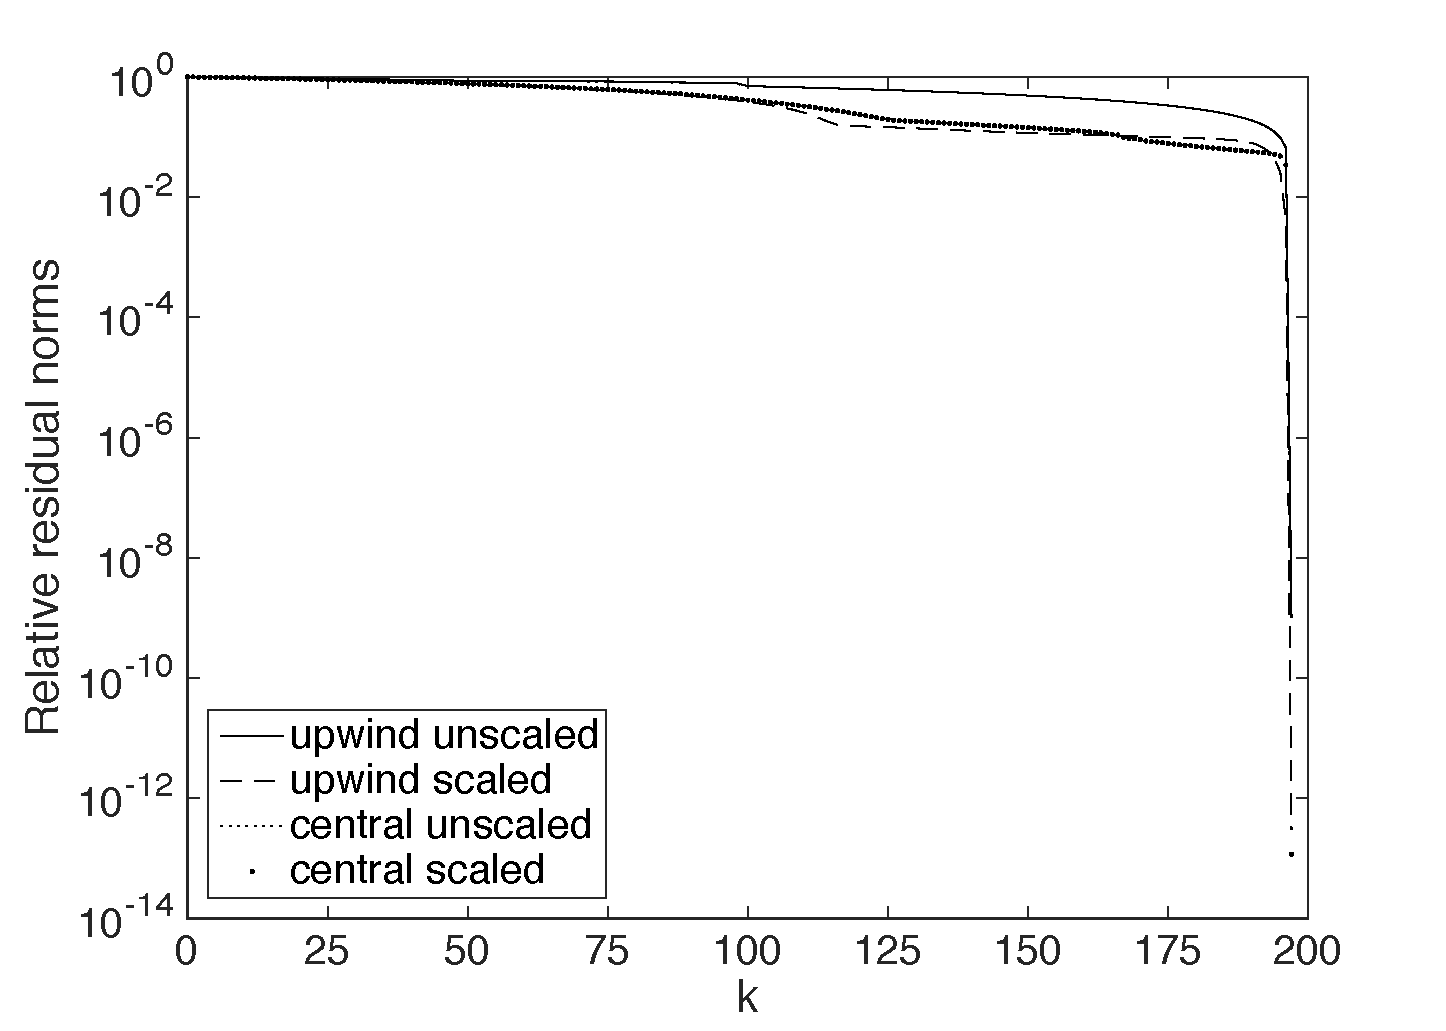
\includegraphics[width=0.95\linewidth]{figures/gmres_4_198}
% \caption{GMRES convergence for $\epsilon=10^{-4}$.}\label{fig:back:GMRES.N198.eps4}
% \end{minipage}
% %
% \begin{minipage}[t]{0.48\linewidth}
% 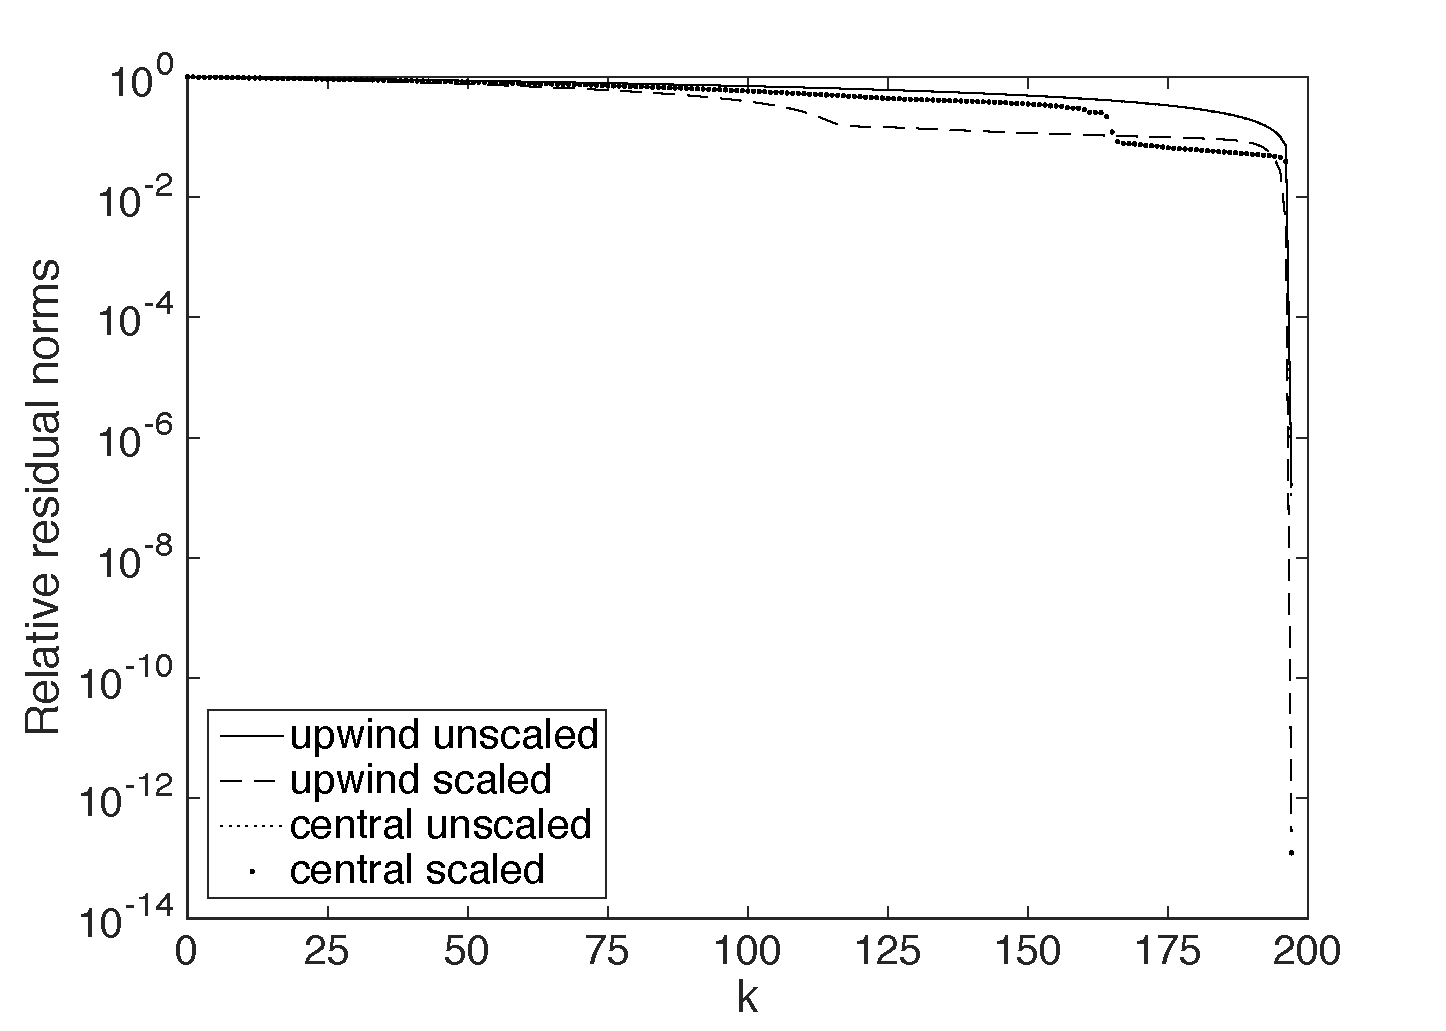
\includegraphics[width=0.95\linewidth]{figures/gmres_6_198}
% \caption{GMRES convergence for $\epsilon=10^{-6}$.}\label{fig:back:GMRES.N198.eps6}
% \end{minipage}
% \end{figure}
% %
% \begin{figure}
% \centering
% \begin{minipage}[t]{0.48\linewidth}
% 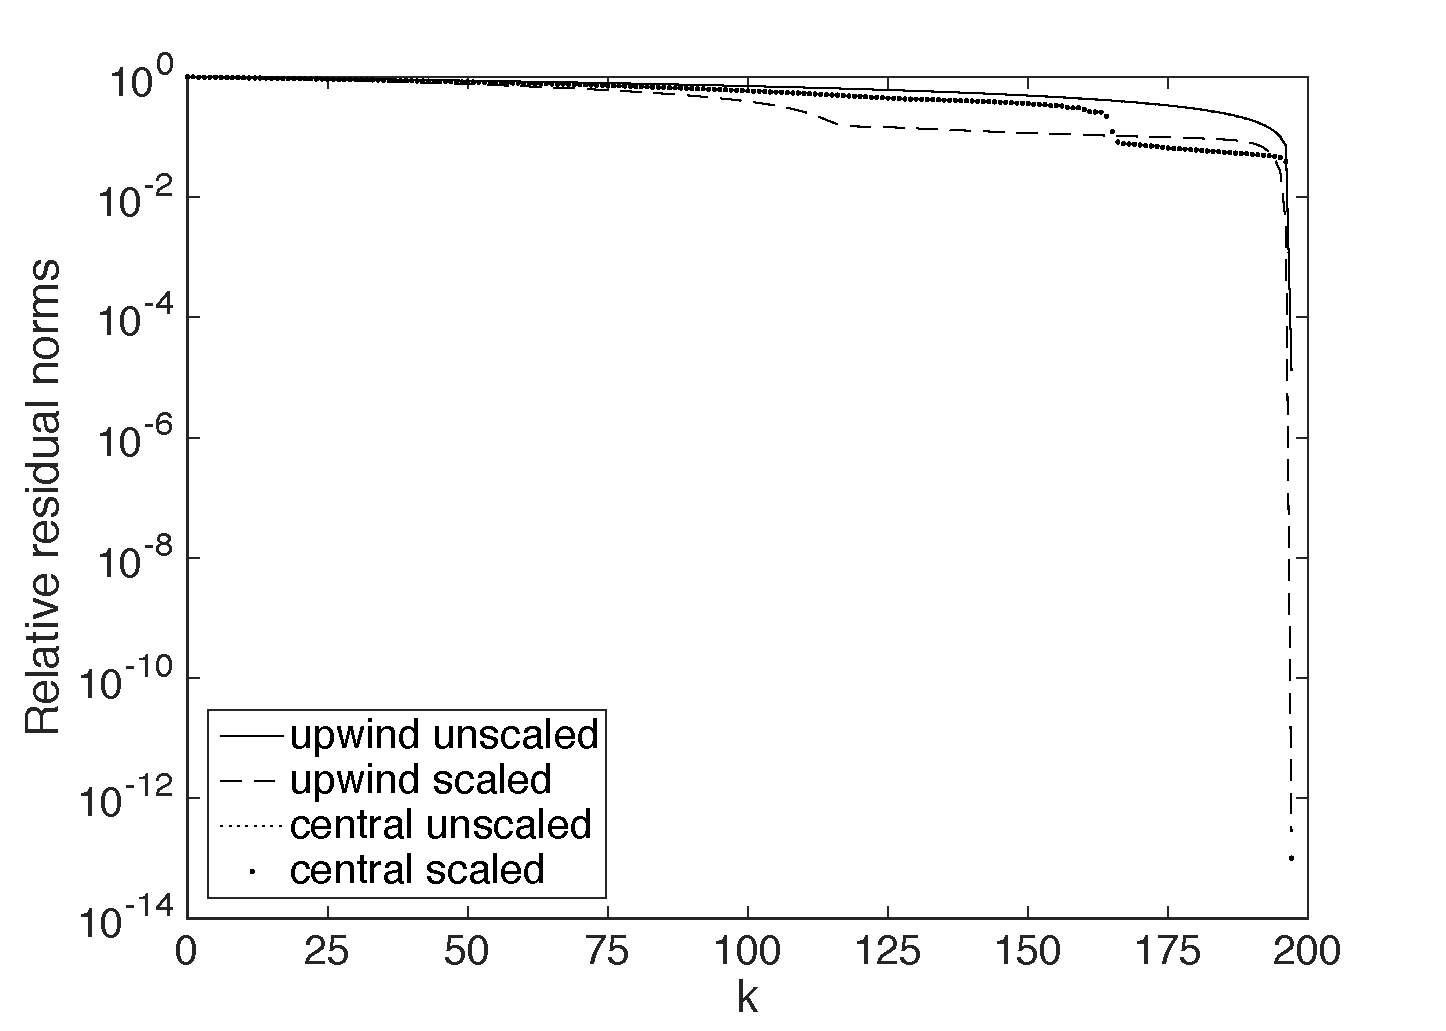
\includegraphics[width=0.95\linewidth]{figures/gmres_8_198}
% \caption{GMRES convergence for $\epsilon=10^{-8}$.}\label{fig:back:GMRES.N198.eps4}
% \end{minipage}
% \end{figure}

In the following, Figures~\ref{fig:back:GMRES.N198.eps4}--\ref{fig:back:GMRES.N198.eps8}
% \td{\textbf{fix:} recompute figures and remove scaled plots.}
illustrate that linear algebraic systems resulting from
discretizations of convection-dominated convection-diffusion problems represent
a challenge for GMRES holds for the Shishkin mesh
discretization of the model problem \eqref{eq:back:1Dbvp}. These figures show
the relative residual norms of the (unpreconditioned) GMRES method with zero
initial vector applied to $\A\u=\f$ from the Shishkin mesh discretization of
\eqref{eq:back:1Dbvp} with $\omega_x=1$, $\beta=0$, $f(x)\equiv 1$, $u_0=u_1=0$,
$N=198$, and different values of $\epsilon$. The GMRES convergence is virtually
the same for both discretizations (upwind and central differences).
 % The eigenvector conditioning does not appear to have a significant effect
% on the performance of the iterative solver.

% \begin{figure}[h!]
% \begin{minipage}[t]{0.48\linewidth}
% 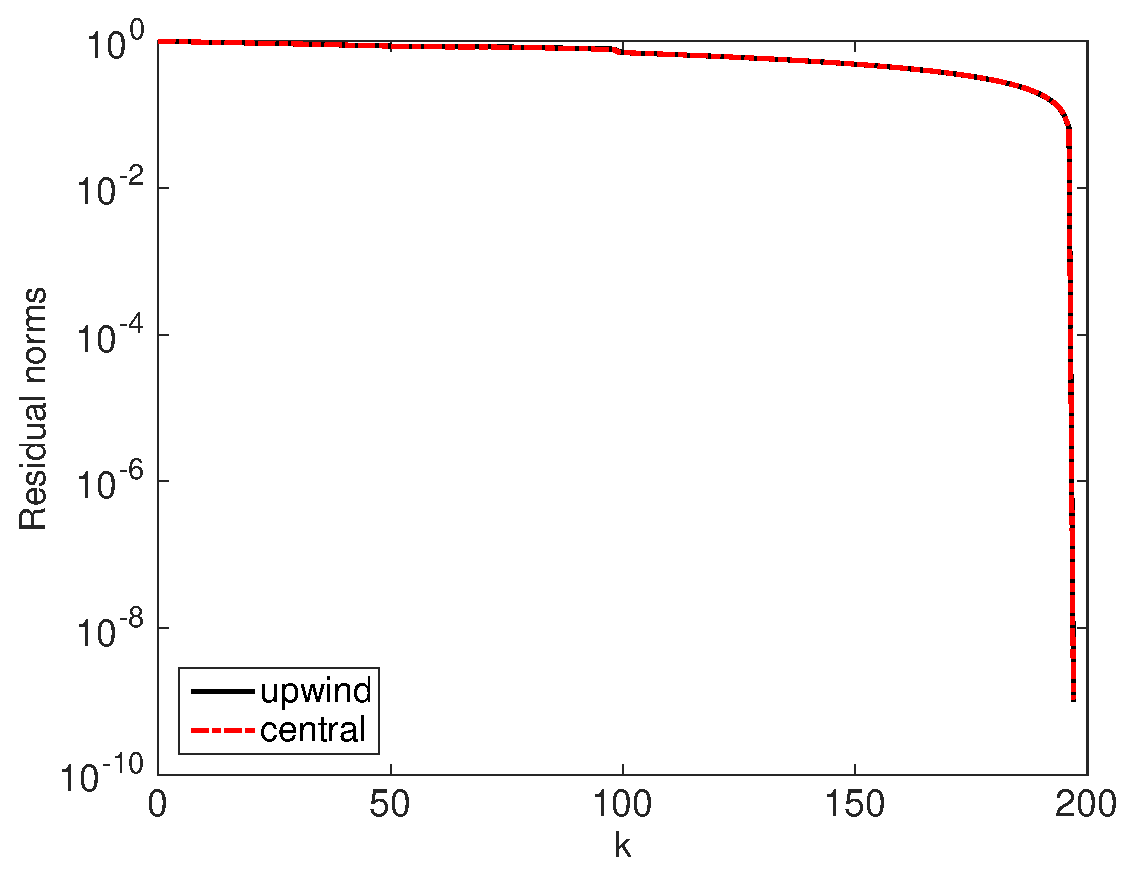
\includegraphics[width=0.95\linewidth]{figures/gmres_eps_1e-04_N_198}
% \caption{GMRES convergence for $\epsilon~=~10^{-4}$.}
% \label{fig:back:GMRES.N198.eps4}
% \end{minipage}
% %
% \begin{minipage}[t]{0.48\linewidth}
% 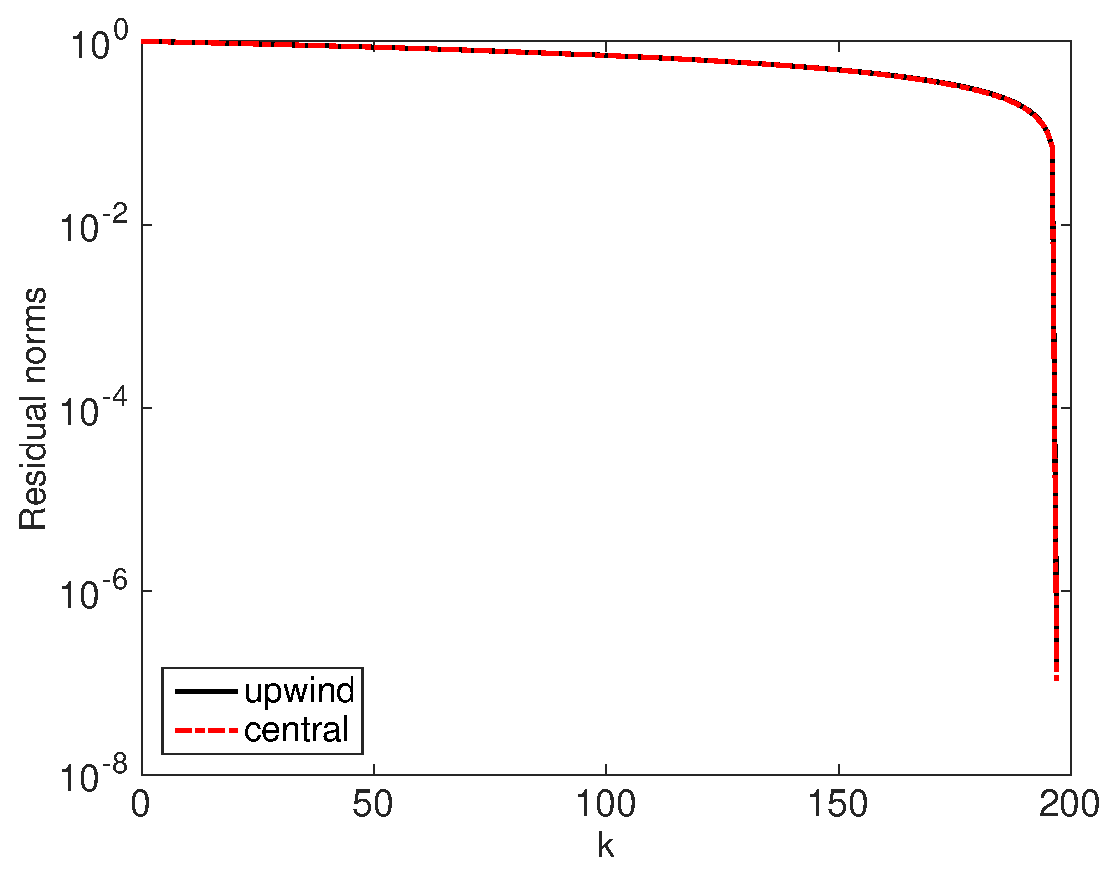
\includegraphics[width=0.95\linewidth]{figures/gmres_eps_1e-06_N_198}
% \caption{GMRES convergence for $\epsilon~=~10^{-6}$.}
% \label{fig:back:GMRES.N198.eps6}
% \end{minipage}
% %\caption{GMRES convergence for $\epsilon~=~10^{-4}$.}[left] and $\epsilon~=~10^{-6}$[right].}\label{fig:back:GMRES.N198.eps6}
% \end{figure}
%

\begin{figure}[h!]
\begin{minipage}[t]{0.48\linewidth}
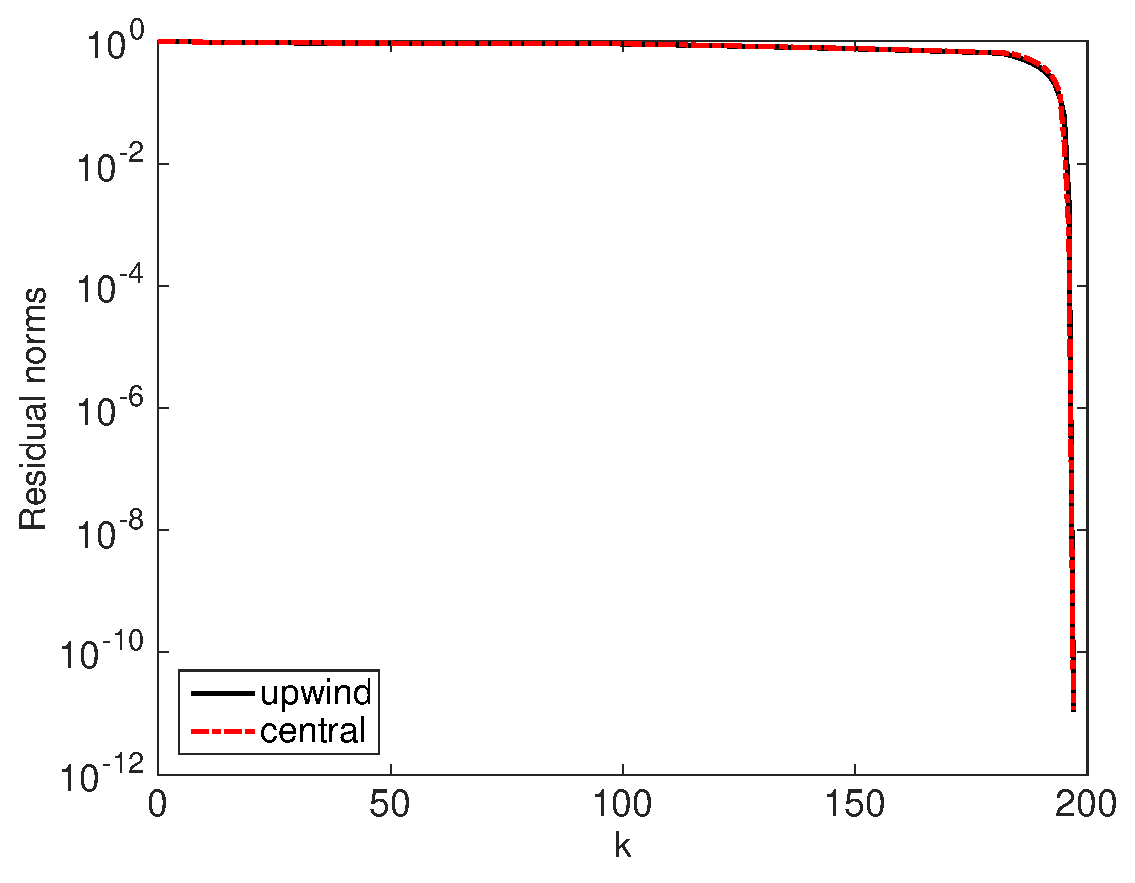
\includegraphics[width=0.98\linewidth]{figures/gmres_eps_1e-02_N_198}
%\label{fig:1D:GMRES.N198.eps4.prec}
% note: if changing to 3 figures again, it needs to be changed in two places
%\caption{Preconditioned GMRES convergence for $\epsilon=10^{-4}$.}
\end{minipage}
%
\begin{minipage}[t]{0.48\linewidth}
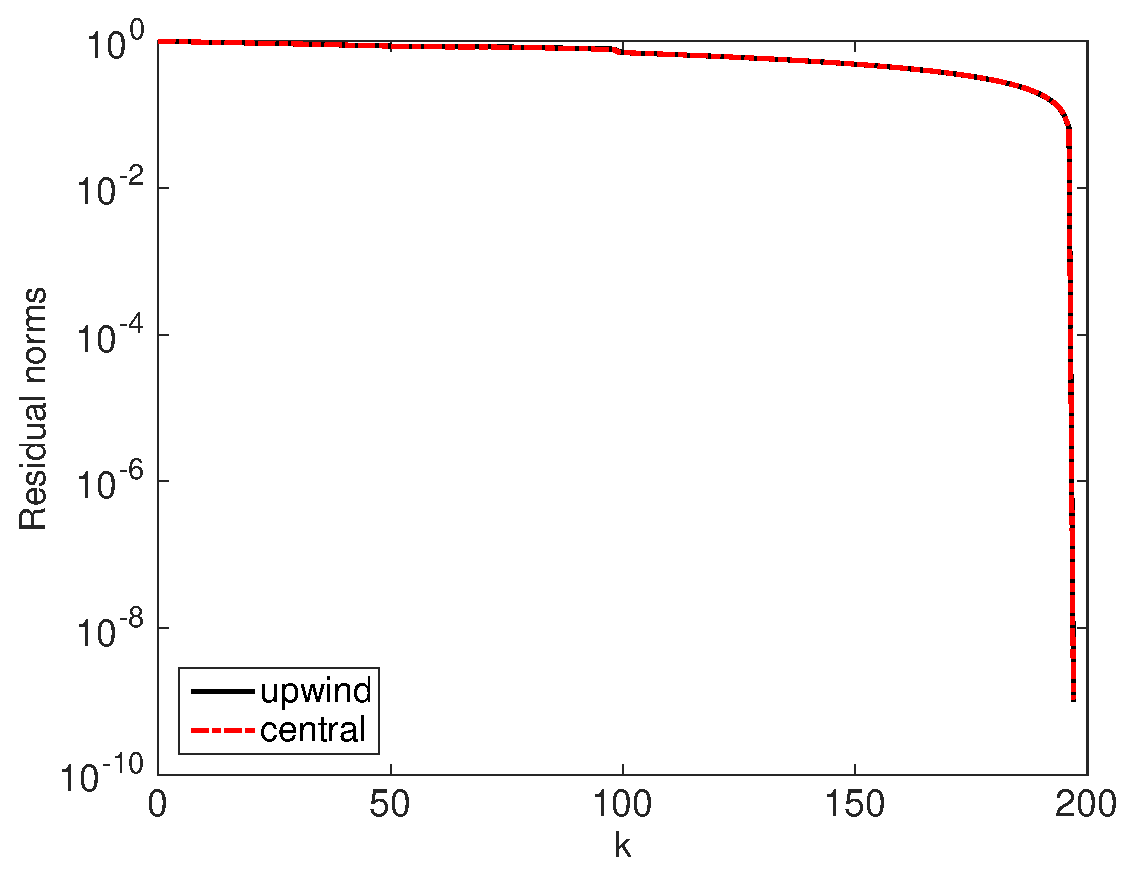
\includegraphics[width=0.98\linewidth]{figures/gmres_eps_1e-04_N_198}
\end{minipage}
\caption{GMRES convergence for $\epsilon=10^{-2}$ and $\epsilon=10^{-4}$ [r].}
\label{fig:back:GMRES.N198.eps4}
\end{figure}
%
\begin{figure}[h!]
\begin{minipage}[t]{0.48\linewidth}
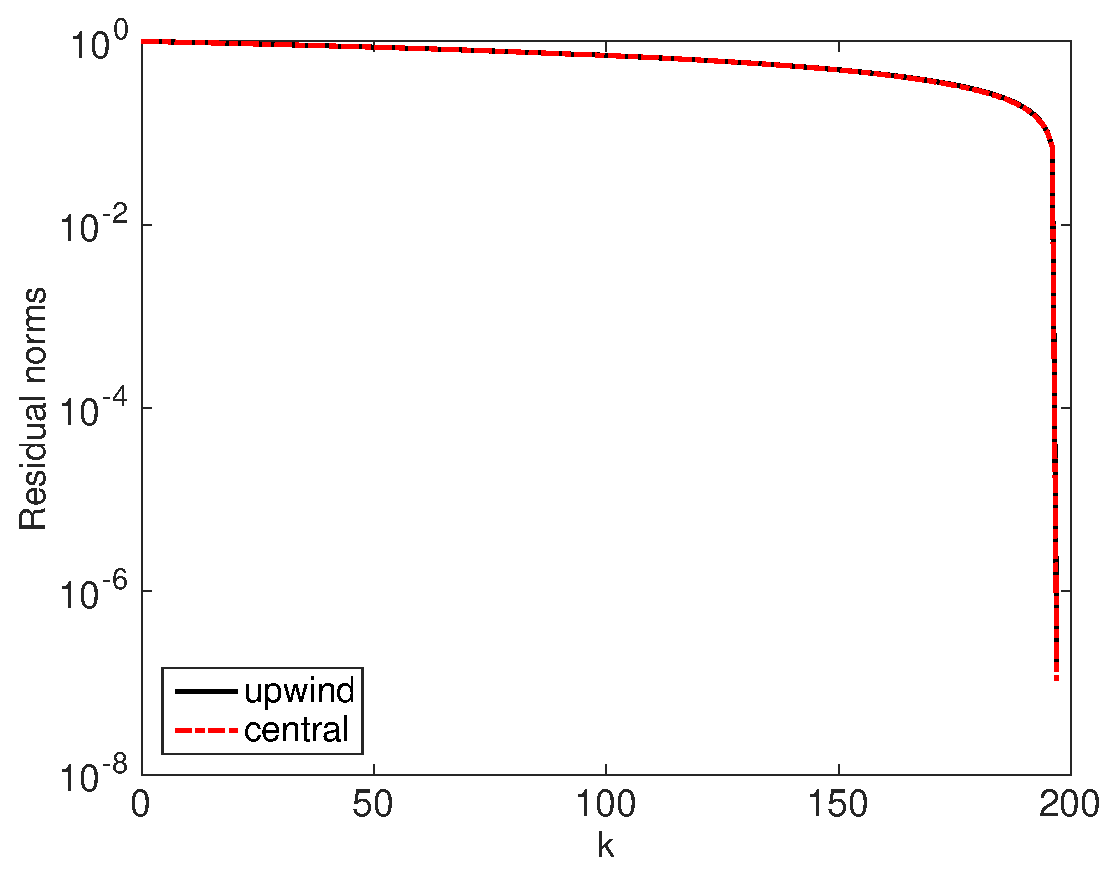
\includegraphics[width=0.98\linewidth]{figures/gmres_eps_1e-06_N_198}
%\label{fig:1D:GMRES.N198.eps4.prec}
% note: if changing to 3 figures again, it needs to be changed in two places
%\caption{Preconditioned GMRES convergence for $\epsilon=10^{-4}$.}
\end{minipage}
%
\begin{minipage}[t]{0.48\linewidth}
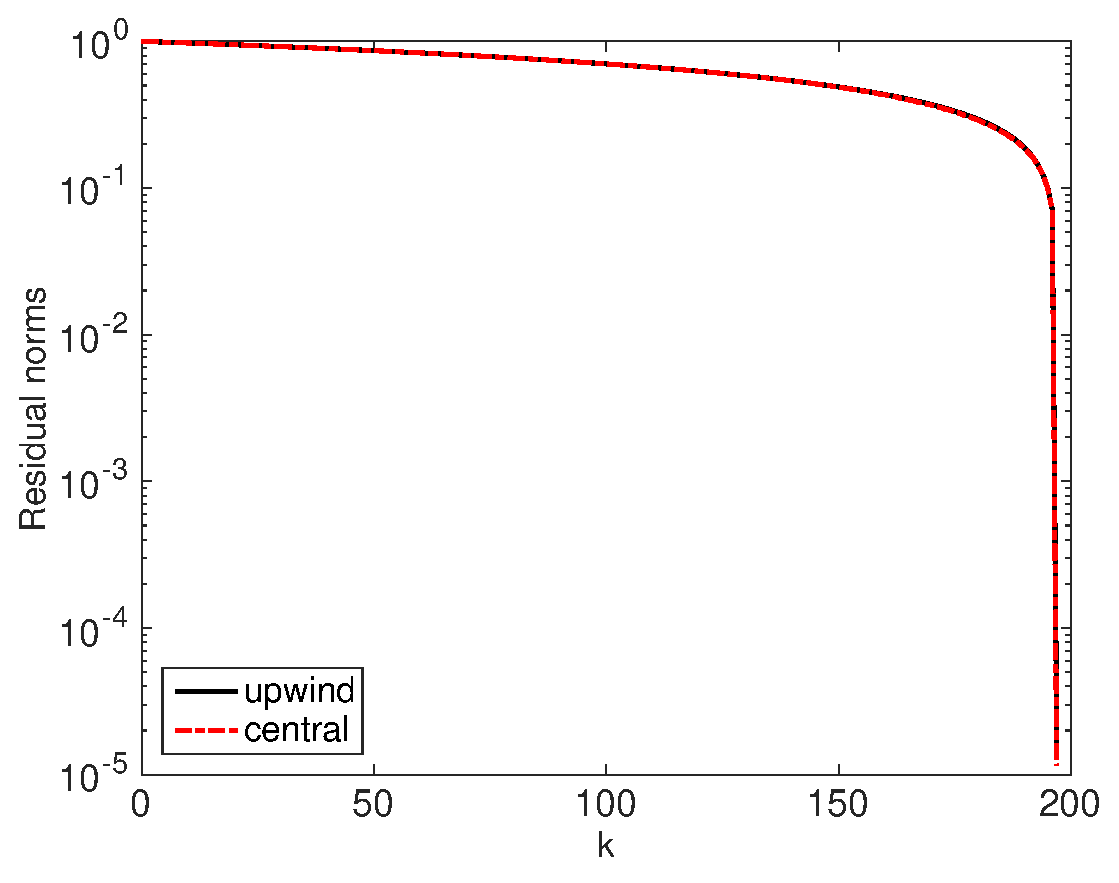
\includegraphics[width=0.98\linewidth]{figures/gmres_eps_1e-08_N_198}
\end{minipage}
\caption{Preconditioned GMRES convergence for $\epsilon=10^{-6}$ and $\epsilon=10^{-8}$ [r].}
\label{fig:back:GMRES.N198.eps8}
\end{figure}

% \begin{figure}
% \centering
% \begin{minipage}[t]{0.48\linewidth}
% 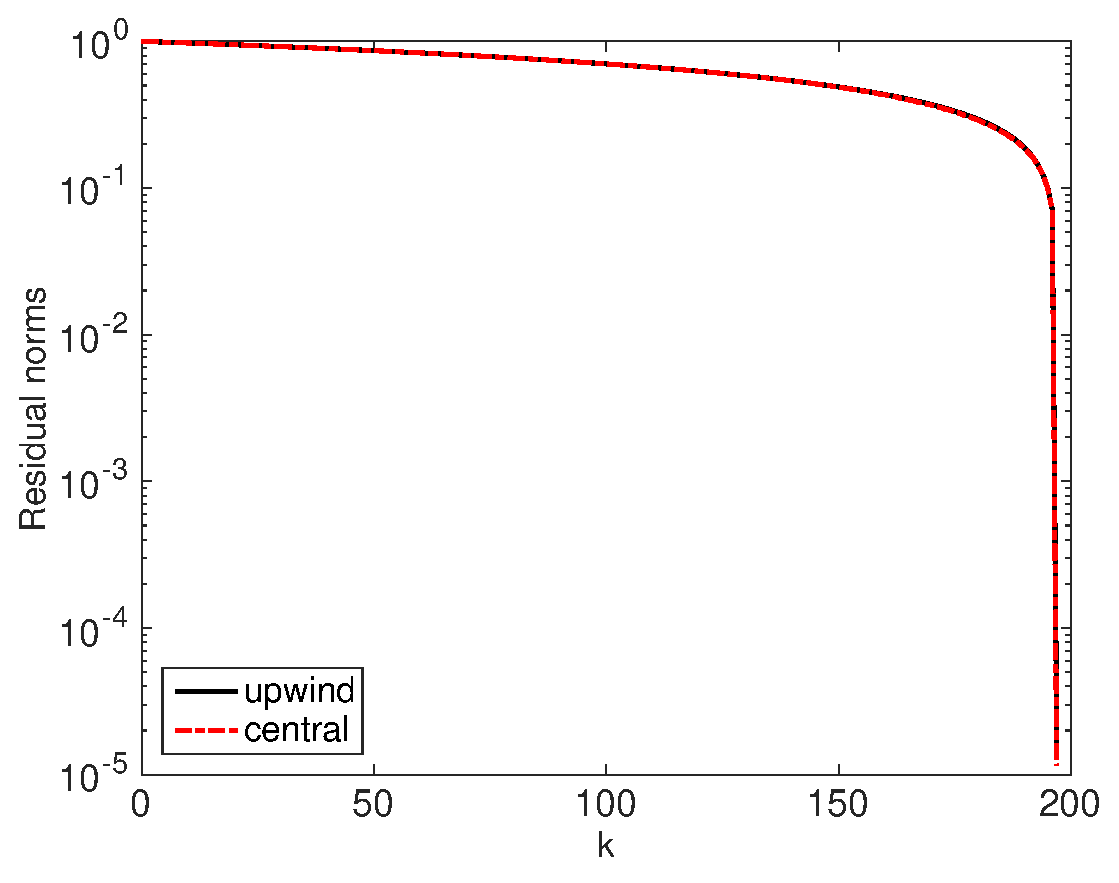
\includegraphics[width=0.95\linewidth]{figures/gmres_eps_1e-08_N_198}
% \caption{GMRES convergence for $\epsilon~=~10^{-8}$.}
% \label{fig:back:GMRES.N198.eps8}
% \end{minipage}
% \end{figure}

For the problems studied in this thesis, the eigenvector basis of the
coefficient matrix $\A$ is very badly conditioned, making the matrix highly
\emph{nonnormal}. In such cases, the use of eigenvalues and eigenvectors in an
analysis of convergence is not informative and very poorly descriptive, see for
example \cite{GreStrPta96} for an extreme case where this is true and \cite{Ern00} for an example of a convection-diffusion problem for which the eigenvalues alone give misleading information about convergence.
% \td{\textbf{add}:a good citation for this asseveration is needed (Eiermann, Ernst?)}.
% In the case of nonnormal matrices $A$, the standard approach to the GMRES
% convergence analysis is noninformative and hardly descriptive.
Such analysis use the eigendecomposition of the coefficient matrix,
$\A=\Y\D\Y^{-1}$, where $\D$ is a diagonal matrix whose elements contain the
eigenvalues $\lambda_k$ of $\A$, and is given by
\begin{align}
\|\r^{(n)}\|&=\|\Y p_n(\D) \Y^{-1}\r^{(0)}\|=\min_{p\in \pi_n}\|\Y p(\D)\Y^{-1}\r^{(0)}\|\\
&\leq\|\Y\|\|\Y^{-1}\|\|\r^{(0)}\|\min_{p \in \pi_n}\max_k|p(\lambda_k)|.
\end{align}
This result is a worst case bound that does not take into account the fact that
for some initial residuals GMRES may behave very differently than for others.
It simplifies the analysis by separating the study of GMRES convergence
behavior into optimizing the condition number of the eigenvector matrix $\Y$ and
a polynomial minimization problem over the spectrum of $\A$, but it could
potentially overestimate GMRES residuals. This is partly because, as observed
by Liesen and Strakos in \cite{LieStr03}, possible cancellations of huge
components in $\Y$ and/or $\Y^{-1}$ are artificially ignored for the sake of the
convergence analysis.

% \begin{figure}[h!]
% \centering
% 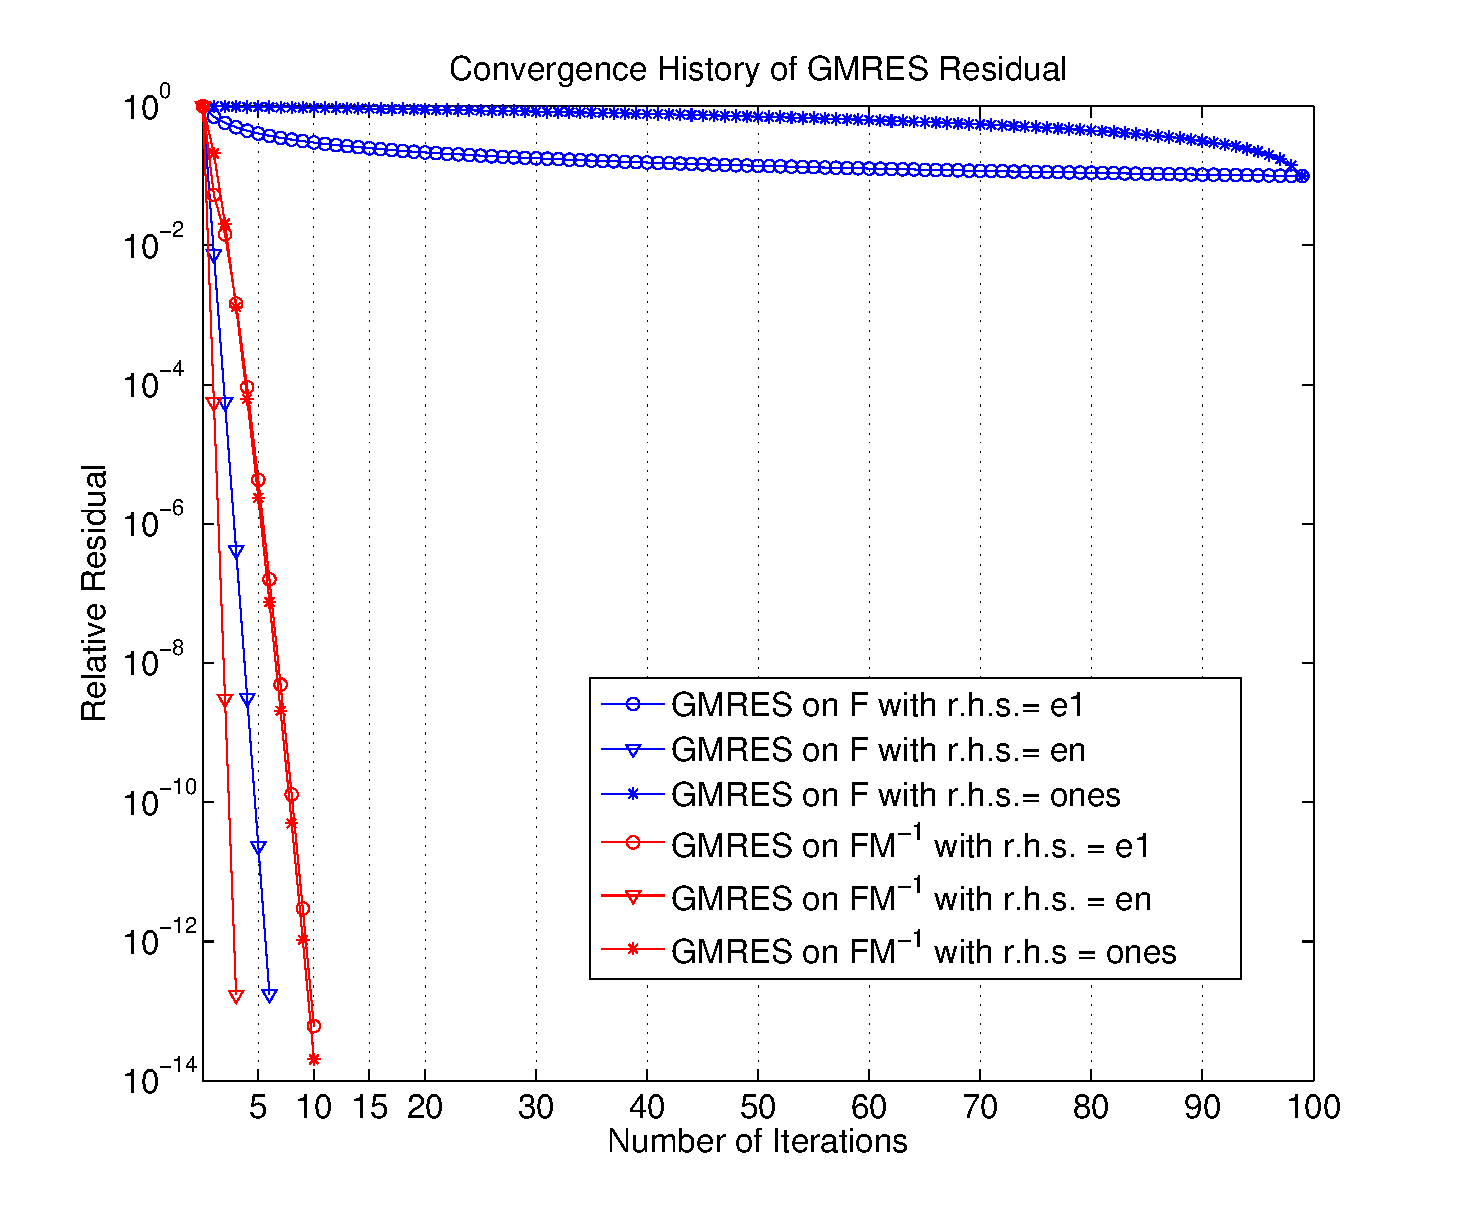
\includegraphics[scale=0.25]{figures/convergence2.eps}
% %\vspace*{-1em}
% 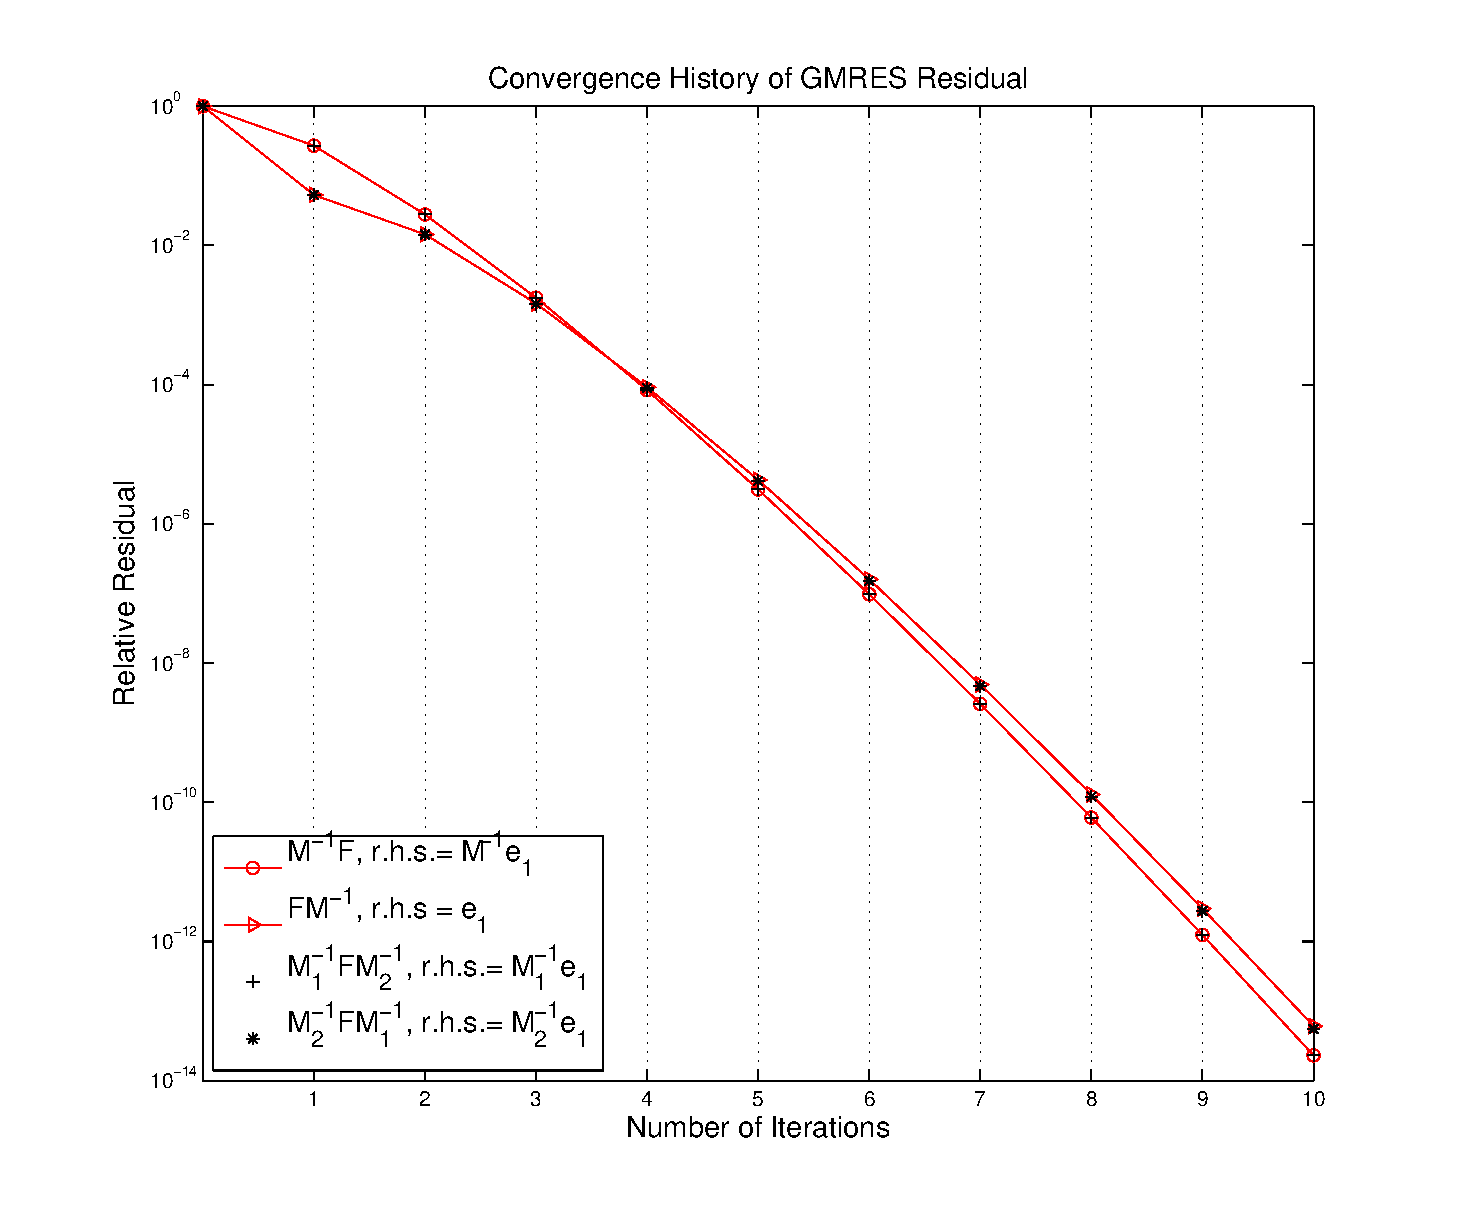
\includegraphics[scale=0.25]{figures/Convergence_e1}
% \caption{GMRES convergence history for the right-preconditioned and
% unpreconditioned systems.}
% \label{fig:back:1DConvergence}
% \end{figure}

The stagantion of GMRES for solving convection-diffusion problems of type \eqref{eq:back:1Dbvp} and \eqref{eq:back:nDbvp} shows the need to either find a preconditioning strategy to accelerate the convergence of the method or the use of a completely different solution approach to solve these types of problems. In the following we will discuss another type of solution methods which fall under the category of domain decomposition methods, which seem to be a natural solution for the types of problems studied in this thesis.


\subsection{Domain Decomposition and Schwarz Methods}
\label{back:itersolvers:DDM}

The earliest know domain decomposition method is believed to have been
discovered in 1869 by Hermann Amandus Schwarz in \cite{Sch69}. Schwarz devised
the method for elliptic equations, to establish the existence of harmonic
functions on regions with nonsmooth boundaries. Throughout the 20th century, the area of domain decomposition methods has grown extensively and a variety of methods have been introduced, both at the continuous level as well at the algebraic level; see \cite{BenFroNabSzy01} for the theory of algebraic methods and \cite{SmiBjoGro96} for a complete monograph of domain decomposition methods. Our focus in this work will fall in the algebraic case, commonly known as the multiplicative Schwarz method, however we will describe Schwarz' original idea in the following (see \cite{GanWan14} for a historical introduction to the method).
% \td{\textbf{note}: remeber to read and cite Gander's paper on Helmholtz \cite{GanZha19}}


\subsubsection{2.2.3.1. \ The Continuous Case: Schwarz's Alternating Procedure}
\label{back:itersolvers:DDM:AltSchwarz}

When the alternating Schwarz method is considered at the continuous level,
there are two main variants to be considered. The first one being the original
method invented by Schwarz in \cite{Sch69} at the end of the 19th century as a
mathematical tool for investigating the uniqueness of the solution to the
Laplace equation when it is posed on a general complex domain, and the  second
one being the parallel Schwarz method used in the general area of parallel
computing, which was introduced by Lions in the 1980's. We will briefly
describe the first one and direct the reader to the complete review paper by
Gander in \cite{Gan08} which gives a thorough analysis of Schwarz methods
over the course of time.

\begin{figure}[h!]
\centering
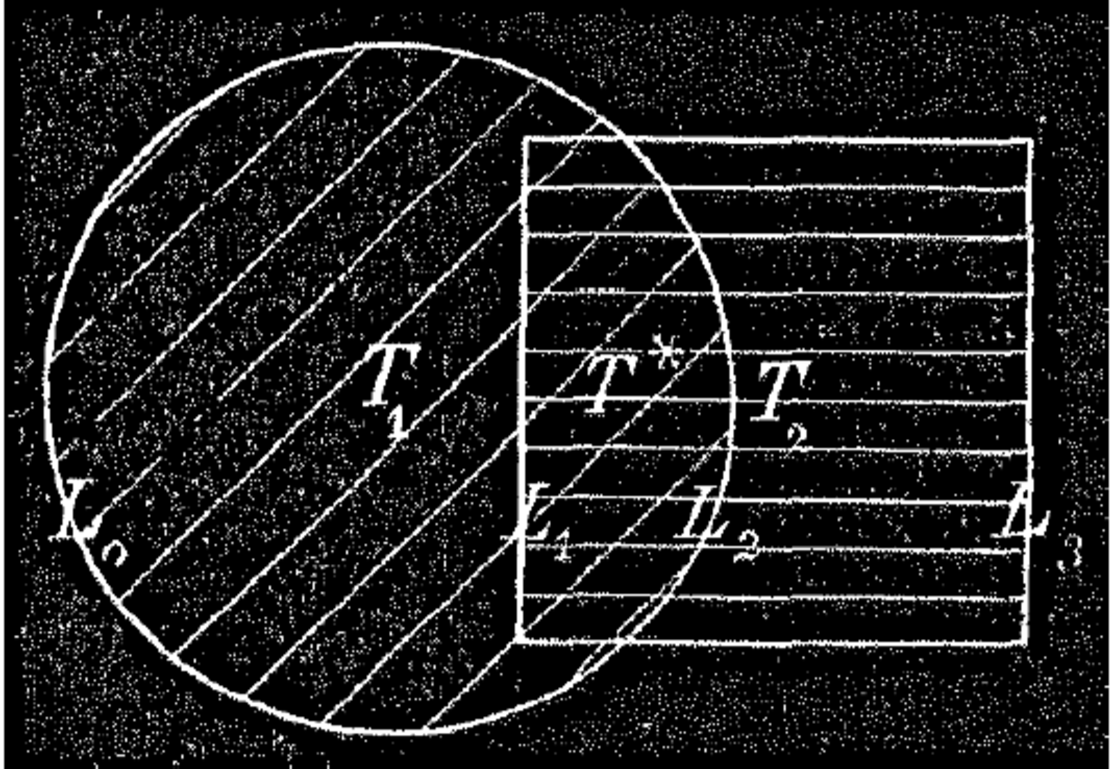
\includegraphics[scale=0.25]{figures/original_domain.pdf}
\caption{Original domain used by Schwarz consisting of a disk and a rectangle.}
\label{fig:back:orig_domain}
\end{figure}

Even though the scientific agenda at the time sought to find a proof of the uniqueness and existence of solutions for Laplace's equation posed on a general complex domain, Schwarz focused on first finding the solution on a domain that was composed of two simpler domains for which existence and uniqueness had already been proven. Figure~\ref{fig:back:orig_domain} shows the original domain used by Schwarz for his analysis, which consisted of a disk $\Omega_1$ (labeled $T_1$ in the figure) "stitched" together with a rectangle $\Omega_2$ (labeled $T_2$ in the figure). The project was to show that the following BVP
%
\begin{equation}\label{eq:back:Laplace}
\mathscr{A}u\equiv\Delta u=0,\text{ in }\Omega,\quad u=g\text{ on }\partial\Omega,
\end{equation}
%
holds for an arbitrary choice of Dirichlet boundary conditions.
Since the solutions on each subdomain were known using Fourier series,
Schwarz proposed an iterative solution scheme for the entire domain which only made use of the known solutions on the disk and the rectangle.
Providing an initial guess $u_0^2$ along $\Gamma_1\equiv\partial\Omega_1\cap\Omega_2$, the iteration computes the approximations $u_1^{n+1}$ and $u_2^{n+1}$ on each subdomain as follows:
\begin{equation}\label{eq:back:AltSchwarz}
\begin{array}{cc}
\Delta u_1^{n+1} = 0 \text{ in } \Omega_1, & \Delta u_2^{n+1} = 0 \text{ in } \Omega_2,\\
u_1^{n+1} = u_2^{n} \text{ on } \Gamma_1, & u_2^{n+1} = u_1^{n+1} \text{ on } \Gamma_2,
\end{array}
\end{equation}
where $\Gamma_2\equiv\partial\Omega_2\cap\Omega_1$ and both $u_1^{n+1}$ and $u_2^{n+1}$ satisfy the given Dirichlet conditions on the outer boundaries of each subdomain. The convergence of the previous algorithm to the solution of the problem was proven by Schwarz using a maximum principle and very loosely consisted in introducing artificial boundaries for each subdomain (given by the overlap) and using them as Dirichlet conditions for the second subdomain in order to solve each problem in an alternating fashion. For the specific proof, we direct the reader to the original paper by Schwarz in \cite{Sch69} or the survey paper \cite{Gan08}. We will next present the algebraic case, which is the main method of analysis in this thesis.

\subsubsection{2.2.3.2. \ The Discrete (Algebraic) Case: The Multiplicative Schwarz Method}
\label{back:itersolvers:DDM:MultSchwarz}

Schwarz methods have also been introduced directly at the algebraic level for
solving the linear system $\A\u=\f$, and there are several variants. We will now
describe one of them: the multiplicative Schwarz method (see \cite{BenFroNabSzy01}). In short, the method
uses restriction operators for constructing a multiplicative iteration matrix
in which each factor corresponds to a local solve in one of the subdomains.

% The multiplicative Schwarz method for solving linear algebraic systems of the
% form \eqref{eq:linsys} uses restriction operators for constructing a
% multiplicative iteration matrix, where each factor corresponds to a local solve
% in one of the subdomains $\Omega_1$ and $\Omega_2$.

\begin{figure}[h]
\centering
% \begin{tikzpicture}
%  % \tikzset{
%  %   elps/.style 2 args={draw, ellipse,minimum width=#1, minimum height=#2},
%  %   node distance=1.8 cm,
%  %   font=\footnotesize,
%  %   >=latex,
%  %   bullet/.style = {circle, inner sep=1pt, fill}
%  % }
%     \draw [gray!50]  (0,0) -- (1,1) -- (3,1) -- (5,0.9)  -- (5,-1) -- cycle;
%     \draw [red] plot [smooth cycle] coordinates {(0,0) (1,1) (3,1) (5,1) (5,-1)};
%     % \node(a)[elps={3cm}{1.5cm},label={below:$\Omega$}]
%     %    [path picture=\ppfill{white}{white}]{};
%     \node at (-1.0,0.2) {$\Omega_{1}$};
%     \node at (0.1,0.35) {$\Gamma_{12}$};
%     \node at (1.0,-0.2) {$\Omega_{2}$};%
%
% \end{tikzpicture}
\begin{turn}{90}
\begin{tikzpicture}[scale=0.06]
\draw (0, 0) .. controls (5.18756, -26.8353) and (60.36073, -18.40036)
   .. (60, 40) .. controls (59.87714, 59.889) and (57.33896, 81.64203)
   .. (40, 90) .. controls (22.39987, 98.48387) and (4.72404, 84.46368)
   .. (10, 70) .. controls (13.38637, 60.7165) and (26.35591, 59.1351)
   .. (30, 50) .. controls (39.19409, 26.95198) and (-4.10555, 21.23804)
   .. (0, 0);
\draw (30.7,40.0) -- (60.0,40.0);
\begin{turn}{-90}
\node at (-10,26) {$\Omega_{2}$};
\node at (-30,45) {$\Gamma_{12}$};
\node at (-75,26) {$\Omega_{1}$};
\end{turn}
\end{tikzpicture}
\end{turn}
\vspace*{-5cm}
\caption{Decomposition of a domain $\Omega$ into two local subdomains $\Omega_1$ and $\Omega_2$ with interface boundary $\Gamma_{12}$.}
\label{fig:back:2DSchwarzdomain}
\end{figure}

% \begin{figure}[h]
% \centering
% \begin{tikzpicture}
%  \tikzset{
%    elps/.style 2 args={draw, ellipse,minimum width=#1, minimum height=#2},
%    node distance=1.8 cm,
%    font=\footnotesize,
%    >=latex,
%    bullet/.style = {circle, inner sep=1pt, fill}
%  }
%
%     \node(a)[elps={3cm}{1.5cm},label={below:$\Omega$}]
%        [path picture=\ppfill{white}{white}]{};
%     \node at (-1.0,0.2) {$\Omega_{1}$};
%     \node at (0.1,0.35) {$\Gamma_{12}$};
%     \node at (1.0,-0.2) {$\Omega_{2}$};%
%
% \end{tikzpicture}
% \caption{Decomposition of a domain $\Omega$ into two local subdomains $\Omega_1$ and %$\Omega_2$ with interface boundary $\Gamma_{12}$.}
% \label{fig:domain}
% \end{figure}

Just like the continuous domain is partitioned into subdomains, the unknowns in the vector $\u$ need to be subdivided into corresponding subsets, possibly overlapping each other. Without loss of generality, and referring to Figure~\ref{fig:back:2DSchwarzdomain}, %\td{\textbf{fix:} write a TIkz figure with a generic domain},
we consider one domain, $\Omega$, subdivided into two contiguous local subdomains, $\Omega_1$ and $\Omega_2$, by one interface boundary $\Gamma_{12}$. The only assumption we make is that in each of the local subdomains we have the same number of unknowns. This assumption is made for simplicity of the following exposition. Extensions to other block sizes and several subdomains are certainly possible, but would require even more technicalities. In this context, the restriction operators can be written as
% \td{\textbf{write}: mention that the analysis can be extended to any number of domains and therefore we will have as many number of projectors}
%
$$\R_1\equiv \left[\I_{n}\quad 0 \right]\quad\mbox{and}\quad \R_2\equiv \left[0\quad  \I_{n} \right],$$
%
both of size $n\times (N-1)$.
%\td{\textbf{fix}: the notation $\I_{\text{size}}$ is not used after this point - change the rest so that it does. To be consistent we also need a $\mathbf{0}$ to represent the array of zeros too}
Therefore the operation $\R_1\u$ yields the
unknowns in the first subset while $\R_2\u$ delivers the unknowns of the second
subset (subdomain). The corresponding unknowns in the matrix $\A$ can be
obtained using the same restriction operators and thus, the restrictions of the
matrix $\A$ in $\A\u=\f$ to the two subdomains are given by the two $n\times n$
matrices
%
\begin{equation}\label{eq:back:local_prob}
\matA_1 \equiv \R_1\A\R_1^T \equiv
\left[\begin{array}{cc}
\matAH &\entryvE  \e_{m }\\
\entryzW \e_{m}^T& \entryzC
\end{array}\right]
\quad\mbox{and}\quad
\matA_2\equiv \R_2\A\R_2^T\equiv
\left[\begin{array}{cc}
\entryzC &\entryzE \e_{1}^T\\
\entrywW \e_{1}& \matAh
\end{array}\right],
\end{equation}
%
where $m\equiv n-1$, and $\e_1,\e_m\in {\mathbb R}^m$. In the following, the
unit basis vectors $e_j$ are always considered to be of appropriate length,
which for simplicity is sometimes not explicitly stated. Note that
$\matAH, \matAh\in \mathbb{R}^{m\times m}$ are tridiagonal Toeplitz matrices.
The matrices corresponding to the solves on the two domains then are given by
%
\begin{equation}\label{eq:back:Pi}
\P_i\equiv \R_i^T\A_i^{-1}\R_i\A,\quad i=1,2.
\end{equation}
%
It is easy to see that $\P_i^2=\P_i$, i.e., that these matrices are projections.
Note also that since $\P_i$ is not symmetric, we have for the 2-norm,
that $\|\I-\P_i\|_2 = \|\P_i\|_2 > 1$; see, e.g., \cite{Szy06}. Using the
complimentary projections
%
$$\Q_i\equiv \I-\P_i\;\in\;\mathbb{F}^{(N-1)\times (M-1)},\quad i=1,2,$$
%
we define the multiplicative Schwarz iteration matrices
%
\begin{equation}\label{eq:back:Tij}
\T_{12}\equiv \Q_2\Q_1\quad\mbox{and}\quad \T_{21}\equiv \Q_1\Q_2.
\end{equation}
%
Thus, $\T_{ij}$ corresponds to first solving on $\Omega_i$, and then on
$\Omega_j$. Both iteration matrices will be analyzed below.

Starting with an initial vector $\u^{(0)}\in{\mathbb R}^{N(2m+ 1)}$,
%$\hat{\u}^{(0)}=[\hat{u}_1^{(0)},\hat{u}_2^{(0)},\ldots,\hat{u}_{2m+1}^{(0)}]\in{\mathbb R}^{N(2m+ 1)}$
the multiplicative Schwarz method is defined by
%
\begin{equation}\label{eq:back:schwarz}
\u^{(k+1)}=\T_{ij} \u^{(k)}+\vv, \quad k=0,1,2,\dots,
\end{equation}
%
where $\T_{ij}=\T_{12}$ or $\T_{ij}=\T_{21}$, and the vector
$\vv\in {\mathbb R}^{N-1}$ is defined to make the method consistent.
For the iteration matrix $\T=\T_{ij}$ the consistency condition
$\u=\T_{ij}\u+\vv$ yields
$$
\vv = (\I-\T_{ij})\u = (\P_i+\P_j-\P_j\P_i)\u,
$$
which is (easily) computable since
$$
\P_i\u=\R_i^{\Tr}\A_i^{-1}\R_i\A\u=\R_i^{\Tr}\A_i^{-1}\R_i\f,\quad i=1,2.
$$

The error of the multiplicative Schwarz iteration~\eqref{eq:back:schwarz} is
given by
\begin{equation}\label{eq:back:schwarz_err}
\e^{(k+1)}=\u-\u^{(k+1)}=(\T_{ij}\u + \vv)- (\T_{ij} \u^{(k)}+\vv)=\T_{ij} \e^{(k)},
\quad k=0,1,2,\dots,
\end{equation}
and hence $\e^{(k+1)}=\T_{ij}^{k+1} \e^{(0)}$ by induction.
For any consistent norm $\|\cdot\|$, we therefore have the error bound
%
\begin{equation}\label{eq:back:error}
\|\e^{(k+1)}\|\leq \|\T_{ij}^{k+1}\|\,\|\e^{(0)}\|.
%\leq \|T_{ij}\|^{k+1}\,\|e^{(0)}\|.
\end{equation}
%
Our main goal on the following chapters of this work is the derivation of
quantitative convergence bounds for the error of the multiplicative Schwarz method, where we consider both
$\T_{ij}=\T_{12}$ and $\T_{ij}=\T_{21}$.
%$\T_{12}~=~(\I~-~\P_2)(\I~-~\P_1)$ and $\T_{21}~=~(\I~-~\P_1)(\I~-~\P_2)$.

% We point out that the analysis of the multiplicative Schwarz method
% in the following sections uses the unscaled linear algebraic system with $A$
% as in~\eqref{eq:back:matrix} having the entries~\eqref{eq:back:upwind}
% or~\eqref{eq:back:central}. In Section~\ref{ss:scaling} we explain why this
% analysis also applies to suitably scaled linear algebraic systems, and in
% particular to the scaling suggested by Roos in~\cite{Roo96}.


\fi % end of if statement regarding content shown
